\documentclass[
	12pt,
	%draft, % show overfull hboxes
	]{scrartcl}

\usepackage[    % set up dimensions
	a6paper, 
	landscape,
	left=1.45cm,   
	right=1.45cm,  
	top=1.6cm,
	bottom=1.6cm, 
	%showframe,
	nomarginpar,  % this removes the right margin, centering the text in the middle
	noheadfoot,  % this removes the head and foot margin
	]{geometry}

%\pagestyle{empty}

\newif\iffast
\fastfalse

\usepackage{graphicx}
\usepackage{tikz}
\usetikzlibrary{external}
\usepackage{eso-pic}

% Fonts and encodings
\usepackage[nf]{coelacanth}
\usepackage[T1]{fontenc}

\usepackage{longtable} % Um Tabellen zu machen, die mehrere Seiten lang sind und einen passenden Seitenumbruch haben.
\usepackage{multicol}
%\usepackage[singlespacing]{setspace} % Zeilenabstand
\usepackage{nicefrac} % für besser aussehende Brüche

\usepackage[object=vectorian]{pgfornament}

% pstricks vs pgf/tikz:
% Originally we used pstricks to draw the background ornaments.
% This had the disadvantage of having to use `latex -> dvips -> ps2pdf` with the correct options to get the background
% graphics to display in the right orientation. The necessary options also varied between MiKTeX and TeXLive :-(.
%
% Since i have more experience with tikz, i decided to use that, because it was easier to position the
% elements (they weren't placed quite correctly with the pstricks version.).

% pgfornament vs eps files
% I wanted to use pgfornament at first because it has everything necessary in one easy package.
% Unfortunately the graphics in pgfornament end up having quite thick strokes. This does not look good at the scales
% we're using the patterns.
% So i downloaded the vectorian files and extracted the patterns manually with Inkscape. This probably leads to a slowdown though.


\AddToShipoutPictureBG{%
\begin{tikzpicture}[remember picture, overlay]
	% pgfornament does give very simple and nice vectorian graphics for tikz.
	% The problem is that the lines are too thick and figure 41 is also slightly cropped.
	% pst-vectorian works very well.
	% we're now using the original files from vectorian exported as eps file
	
	% DEBUGGING grid
	%\draw[line width=0.75pt, color=teal, step=.5cm, xshift=0.08cm, yshift=0.43cm] (current page.south west) grid ++(14.85cm,10.5cm);
	% DEBUGGING corners
	%\node [circle, fill=red, minimum size=1pt, xshift=0.0cm, yshift=-0.0cm, scale=0.2] at (current page.north west) {};
	%\node [circle, fill=red, minimum size=1pt, xshift=0.5cm, yshift=-0.5cm, scale=0.2] at (current page.north west) {};
	
	% TODO: This slows down compilation a lot.
	%       Maybe find a faster way to do this.
	\iffast
	\else
	\node[anchor=north west, xshift=0.5cm, yshift=-0.5cm, inner sep=0] at (current page.north west){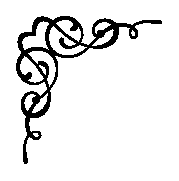
\includegraphics[scale=0.8, angle=0, origin=c]{img/corner_black}};
	\node[anchor=north east, xshift=-0.5cm, yshift=-0.5cm, inner sep=0] at (current page.north east){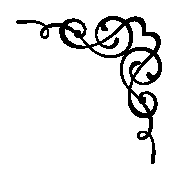
\includegraphics[scale=0.8, angle=0, origin=c]{img/corner2_black}};
	\node[anchor=south west, xshift=0.5cm, yshift=0.5cm, inner sep=0] at (current page.south west){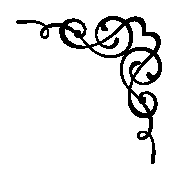
\includegraphics[scale=0.8, angle=180, origin=c]{img/corner2_black}};
	\node[anchor=south east, xshift=-0.5cm, yshift=0.5cm, inner sep=0] at (current page.south east){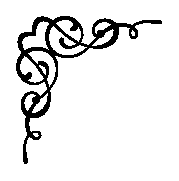
\includegraphics[scale=0.8, angle=180, origin=c]{img/corner_black}};
	\fi
	
	
	% Original pgfornament style:
%	\node[anchor=north west, xshift=0.5cm, yshift=-0.5cm,inner sep=0] at (current page.north west){\pgfornament[scale=0.5]{41}};
%	\node[anchor=north east, xshift=-0.5cm, yshift=-0.5cm, inner sep=0] at (current page.north east){\pgfornament[scale=0.5,symmetry=v]{41}};
%	\node[anchor=south west, xshift=0.5cm, yshift=0.5cm, inner sep=0] at (current page.south west){\pgfornament[scale=0.5,symmetry=h]{41}};
%	\node[anchor=south east, xshift=-0.5cm, yshift=0.5cm, inner sep=0] at (current page.south east){\pgfornament[scale=0.5,symmetry=c]{41}};
	
	% Background as an image, for example a parchment like texture
	%\tikz[remember picture, overlay] \node[opacity=0.5, inner sep=0pt] at (current page.center){\includegraphics[width=\paperwidth,height=\paperheight]{example-image}};
	
\end{tikzpicture}
}

\newcommand{\danceinfo}[1]{%
	{\raggedleft\footnotesize{#1}\par}
}
\newcommand{\dancename}[1]{
	% Dimension are manually chosen so they don't collide with the ornaments in the corners.	
	\begin{tikzpicture}[remember picture, overlay]
%		\node[] at (0, 0) (title) {Text};		
		\node[anchor=north, yshift=-0.5cm, inner sep=0, text width=10.5cm, align=center] at (current page.north){\Huge{#1}};
	\end{tikzpicture}
}
\newcommand{\origininfo}[3]{
	% Dimension are manually chosen so they don't collide with the ornaments in the corners.
	\begin{tikzpicture}[remember picture, overlay]
		% setting the font size in the node options, since it doesn't seem to 
		% take effect when used in the node text. 
		\node[anchor=south west, xshift=1.3cm, yshift=1.15cm, inner sep=0, align=left, font={\scriptsize}] at (current page.south west){Choreographie:\\{#1}};
		\node[anchor=south east, xshift=-1.2cm, yshift=1.15cm, inner sep=0, align=right, font={\scriptsize}] at (current page.south east){Musik:\\ {#2}\\ {#3}};
	\end{tikzpicture}
}
\newcommand{\danceeasymarker}{
	\iffast
	\else
		\begin{tikzpicture}[remember picture, overlay]
			\node[anchor=south, xshift=0cm, yshift=0.5cm, inner sep=0] at (current page.south){\pgfornament[width=4cm]{80}};
		\end{tikzpicture}
	\fi
}
\newcommand{\dancemediummarker}{
	\iffast
	\else
		\begin{tikzpicture}[remember picture, overlay]
			\node[anchor=south, xshift=0cm, yshift=0.5cm, inner sep=0] at (current page.south){\pgfornament[width=5cm]{83}};
		\end{tikzpicture}
	\fi
}
\newcommand{\dancedifficultmarker}{
	\iffast
	\else
		\begin{tikzpicture}[remember picture, overlay]
			\node[anchor=south, xshift=0cm, yshift=0.4cm, inner sep=0] at (current page.south){\pgfornament[width=5cm]{84}};
		\end{tikzpicture}
	\fi
}
\newcommand{\danceinstructionsbegin}{\begin{longtable}{p{1cm}p{9.8cm}}}
\newcommand{\danceinstructionsend}{\end{longtable}}
\newcommand{\danceinstructionsel}{~ & ~ \\}

\setlength{\topskip}{12pt}
\setlength{\parskip}{0pt}

\pagestyle{empty}

\begin{document}

%%%%%%%%%%%%%%%%%%%%%%%%%%%%%%%%%%%%%%%%%%%%%%%%%%%%%%%%%%%%%%%%%%%%%%%%%%%%%%%%
% A Celt's New Dance
%%%%%%%%%%%%%%%%%%%%%%%%%%%%%%%%%%%%%%%%%%%%%%%%%%%%%%%%%%%%%%%%%%%%%%%%%%%%%%%%
%\iffalse
%\newpage
%
%\iffalse\subsection{[A Celt's New Dance]}\fi % fool texstudio into displaying subsections
%
%\dancename{A Celt's New Dance}
%\danceinfo{Grand Square}
%\danceinstructionsbegin
%1 -- 8 & Durchgefasst zum Kreis Meet \& Fall back\\
%9 -- 16 & zum Partner wenden 2-Hände Kette, dann Referenz zum neuen Partner.\\
%1 -- 16 & Wiederholen (Man endet wieder beim eigenen Partner)\\
%\danceinstructionsel
%
%\danceinstructionsend
%%\dancelengthmarker{6}
%%\dancedifficultmarker
%\fi


%%%%%%%%%%%%%%%%%%%%%%%%%%%%%%%%%%%%%%%%%%%%%%%%%%%%%%%%%%%%%%%%%%%%%%%%%%%%%%%%
% An Dro
%%%%%%%%%%%%%%%%%%%%%%%%%%%%%%%%%%%%%%%%%%%%%%%%%%%%%%%%%%%%%%%%%%%%%%%%%%%%%%%%
\newpage

\iffalse\subsection{An Dro}\fi % fool texstudio into displaying subsections

\dancename{An Dro}
\danceinfo{Kette}

~\\
\textit{Kleine Finger haken bei den Nachbarn ein, Arme gesenkt und leicht gebeugt.}
\danceinstructionsbegin
1 -- 4 &	Double links, Hände malen eine 6 aufwärts\\
5 -- 8 &	Double rechts, Hände malen eine 9 abwärts\\
\danceeasymarker
\danceinstructionsend
\textit{Hinweis: Double links wird größer getanzt um vorwärts zu kommen}

%%%%%%%%%%%%%%%%%%%%%%%%%%%%%%%%%%%%%%%%%%%%%%%%%%%%%%%%%%%%%%%%%%%%%%%%%%%%%%%%
% A' Rovin
%%%%%%%%%%%%%%%%%%%%%%%%%%%%%%%%%%%%%%%%%%%%%%%%%%%%%%%%%%%%%%%%%%%%%%%%%%%%%%%%
\newpage

\iffalse\subsection{A' Rovin}\fi % fool texstudio into displaying subsections

\dancename{A' Rovin}
\origininfo{Cecil Sharp ???}{A-Roving / Faithless Nancy Dawson}{Traditional?/Anna Bidder}
\danceinfo{Longway for as many as will}
\danceinstructionsbegin
1 -- 8 	& Paar 1 Lead Down \& Cast Up (lebhaft gesprungen)\\
9 -- 16	& Paar 2 Lead Up \& Cast Down (lebhaft gesprungen)\\
\danceinstructionsel
1 -- 8 	& Dos-á-dos\\
9 -- 16	& Set Rechts zurück und Turn rechts wieder rein\\
\danceinstructionsel
1 -- 8 	& \nicefrac{3}{4} Kette
\danceinstructionsend
\danceeasymarker


%%%%%%%%%%%%%%%%%%%%%%%%%%%%%%%%%%%%%%%%%%%%%%%%%%%%%%%%%%%%%%%%%%%%%%%%%%%%%%%%
% A Trip to Kilburn
%%%%%%%%%%%%%%%%%%%%%%%%%%%%%%%%%%%%%%%%%%%%%%%%%%%%%%%%%%%%%%%%%%%%%%%%%%%%%%%%
\newpage

\dancename{A Trip to Kilburn}
%\subsection{A Trip to Kilburn}
\iffalse\subsection{A Trip to Kilburn}\fi % fool texstudio into displaying subsections
\danceinfo{Longway for as many as will}
\danceinstructionsbegin
1 -- 4 	& FC Settingsteps rechts aufeinander zu\\
5 -- 8 	& FC Settingsteps zurück\\
9 -- 12 & FC Platzwechsel, Klatschen beim dritten Schritt (auf 11)\\
13-- 16 & FC Turn links\\
\danceinstructionsel
1 -- 16 & SC Settingsteps links, Platzwechel, Turn links\\
\danceinstructionsel
1 -- 8 	& Halber Setkreis\\
9 -- 16 & Dos-à-dos\\
\danceinstructionsel
1 -- 8 	& \nicefrac{3}{4} Kette\\
9 -- 16 & Ronde
\dancemediummarker
\danceinstructionsend



%%%%%%%%%%%%%%%%%%%%%%%%%%%%%%%%%%%%%%%%%%%%%%%%%%%%%%%%%%%%%%%%%%%%%%%%%%%%%%%%
% Allemande (Paartanz)
%%%%%%%%%%%%%%%%%%%%%%%%%%%%%%%%%%%%%%%%%%%%%%%%%%%%%%%%%%%%%%%%%%%%%%%%%%%%%%%%
\newpage

\dancename{Allemande}
%\subsection{Allemande}
\iffalse\subsection{Allemande (Paartanz)}\fi % fool texstudio into displaying subsections
\danceinfo{Paartanz}
\textit{Die Dame steht vor dem Herren in der Kiekbuschfassung}\\
\danceinstructionsbegin
1 -- 24 & 3x Chassé links und Chassé rechts, dann wenden\\
%\danceinstructionsel
1 -- 24 & 3x Chassé links und Chassé rechts zurück\\
& \textit{Linke Hände lösen, zueinander wenden}\\
\danceinstructionsel
1 -- 8 	& Das Paar tanzt seitwärts ein kleines Chassé links, dann ein Chassé rechts\\
1 -- 4 	& Schritt kick nach links und rechts\\
5 -- 8 	& Platzwechsel mit Handtour links\\
\danceinstructionsel
& \textit{Rechte Hände loslassen, linke Hände fassen}\\
1 -- 8 & Das Paar tanzt seitwärts ein kleines Chassé links, dann ein Chassé rechts\\
1 -- 4 	& Schritt kick nach rechts und links\\
5 -- 8 	& Die Dame dreht vor dem Herren und nimmt wieder Kiekbuschfassung an.
\dancemediummarker
\danceinstructionsend



%%%%%%%%%%%%%%%%%%%%%%%%%%%%%%%%%%%%%%%%%%%%%%%%%%%%%%%%%%%%%%%%%%%%%%%%%%%%%%%%
% An Improper Notion
%%%%%%%%%%%%%%%%%%%%%%%%%%%%%%%%%%%%%%%%%%%%%%%%%%%%%%%%%%%%%%%%%%%%%%%%%%%%%%%%
\newpage

\dancename{An Improper Notion}
\origininfo{Chris Sackett \& Brooke Friendly (2007)}{An Improper Notion}{von Chris Sackett}
\iffalse\subsection{An Improper Notion}\fi % fool texstudio into displaying subsections
\danceinfo{Longway for as many as will}
\danceinstructionsbegin
1 -- 8 	& Lead Up \& Down\\
1 -- 8 	& Paar 1 Cast Down \& Lead Up, Paar 2 Half-Figure Eight\\
%5 -- 8 	& Paar 1 Lead Up, Paar 2 Cast Down\\
\danceinstructionsel
1 -- 4 	& Set links\\
5 -- 8 	& Paar 1 Cast Down, Paar 2 Lead Up\\
1 -- 4 	& Set links\\
5 -- 8 	& Paar 2 Cast Down, Paar 1 Lead Up\\
9 -- 12 & Paar 1 Cast Down, Paar 2 Lead Up\\
\danceinstructionsel
1 -- 16 & Paar 1 Figure of Eight durch Paar 2\\
\danceinstructionsend
\textit{~~~~~Paar 2 ist abwechselnd proper und improper.}
\dancemediummarker


%%%%%%%%%%%%%%%%%%%%%%%%%%%%%%%%%%%%%%%%%%%%%%%%%%%%%%%%%%%%%%%%%%%%%%%%%%%%%%%%
% Apollo's Hunt
%%%%%%%%%%%%%%%%%%%%%%%%%%%%%%%%%%%%%%%%%%%%%%%%%%%%%%%%%%%%%%%%%%%%%%%%%%%%%%%%
%\newpage
%
%\iffalse\subsection{[Apollo's Hunt]}\fi % fool texstudio into displaying subsections
%\dancename{Apollo's Hunt}
%\danceinfo{Longway for as many as will\\Paar 1 improper}
%\danceinstructionsbegin
%\textbf{Teil} & \textbf{A}\\
%1 -- 8 & Rechthandstern\\
%9 -- 16 & Linkhandstern mit fremdem Set\\
%1 -- 4 & Damen Platzwechsel\\
%5 -- 8 & Herren Platzwechsel\\
%9 -- 16 & Setkreis ganz herum, am Ende Nachbarn anschauen\\
%\danceinstructionsel
%\textbf{Teil} & \textbf{B1}\\
%1 -- 8 & Mirror Image Gypsies: \\
%\textbf{Teil} & \textbf{B2}\\
%
%\danceinstructionsend
%\dancedifficultmarker
%

%%%%%%%%%%%%%%%%%%%%%%%%%%%%%%%%%%%%%%%%%%%%%%%%%%%%%%%%%%%%%%%%%%%%%%%%%%%%%%%%
% Argeers
%%%%%%%%%%%%%%%%%%%%%%%%%%%%%%%%%%%%%%%%%%%%%%%%%%%%%%%%%%%%%%%%%%%%%%%%%%%%%%%%
% \newpage

\iffalse\subsection{[Argeers]}\fi % fool texstudio into displaying subsections
% \dancename{Argeers}
% \danceinfo{}
% \danceinstructionsbegin
% \danceinstructionsend
% \dancedifficultmarker


%%%%%%%%%%%%%%%%%%%%%%%%%%%%%%%%%%%%%%%%%%%%%%%%%%%%%%%%%%%%%%%%%%%%%%%%%%%%%%%%
% Autumn in Amherst
%%%%%%%%%%%%%%%%%%%%%%%%%%%%%%%%%%%%%%%%%%%%%%%%%%%%%%%%%%%%%%%%%%%%%%%%%%%%%%%%
\newpage

\dancename{Autumn in Amherst}
\origininfo{Philippe Callens}{The Red Star Line/Autumn in Amherst}{von Kathy Talvitie}
\iffalse \subsection{Autumn in Amherst}\fi % fool texstudio into displaying subsections
\danceinfo{Longways Duple minor}
\danceinstructionsbegin
1 -- 2 & Einzel rechts\\
3 -- 4 & Referenz\\
5 -- 8 & Drehung links zurück an den Platz\\
1 -- 8 & Handrunde links\\
1 -- 8 & Handrunde rechts mit Gegenpartner\\
1 -- 4 & halber Kreis\\
5 -- 8 & mit dem Gegenpartner paarweise Doppel rückwärts nach außen\\
1 -- 4 & Platztausch Damen auf den Startplatz\\
5 -- 8 & ebenso Herren\\
\danceinstructionsel
\danceinstructionsel
\danceinstructionsel
1 -- 4 & Pousette als halber Kreis\\
5 -- 8 & Pousette senkrecht aus der Gasse und ausfächern - Paare 1 sind aufwärts gerichtet, Paare 2 abwärts\\
1 -- 4 & Doppel vor\\
5 -- 8 & Doppel rückwärts\\
1 -- 4 & Drehung rechts zurück in die Gasse\\
5 -- 8 & Platztausch Partner
\dancemediummarker
\danceinstructionsend



%%%%%%%%%%%%%%%%%%%%%%%%%%%%%%%%%%%%%%%%%%%%%%%%%%%%%%%%%%%%%%%%%%%%%%%%%%%%%%%%
% Blacke Almain
%%%%%%%%%%%%%%%%%%%%%%%%%%%%%%%%%%%%%%%%%%%%%%%%%%%%%%%%%%%%%%%%%%%%%%%%%%%%%%%%
\newpage

\dancename{Black Almain}
\iffalse\subsection{Black Almain}\fi % fool texstudio into displaying subsections
\danceinfo{Kreistanz, Herren innen, in Tanzrichtung}
\danceinstructionsbegin
1 -- 16	& Doppel links, rechts, links, rechts, zueinander drehen\\
%\danceinstructionsel
1 -- 8 	& Doppel links, rechts zurück und vor, dann nach links drehen\\
9 -- 16 & Doppel links vor, um 180° drehen, Doppel rechts zurück, zueinander wenden\\
%\danceinstructionsel
1 -- 8 	& Herr präsentiert sich (z.B. Set \& Turn links)\\
9 -- 16	& Dame präsentiert sich (z.B. Set \& Turn rechts)\\
%\danceinstructionsel
1 -- 4 	& Platzwechsel\\
5 -- 8 	& Seitgalopp in Tanzrichtung\\
1 -- 8 	& Platzwechsel \& Seitgalopp gegen Tanzrichtung\\
%\danceinstructionsel
1 -- 4 	& Doppel links zurück, alle drehen sich zum nächsten andersgeschlechtlichen Partner nach links\\
5 -- 8 	& Doppel rechts vor zum neuen Partner
\dancemediummarker
\danceinstructionsend



%%%%%%%%%%%%%%%%%%%%%%%%%%%%%%%%%%%%%%%%%%%%%%%%%%%%%%%%%%%%%%%%%%%%%%%%%%%%%%%
%	Black Nag
%%%%%%%%%%%%%%%%%%%%%%%%%%%%%%%%%%%%%%%%%%%%%%%%%%%%%%%%%%%%%%%%%%%%%%%%%%%%%%%%
\newpage

\dancename{Black Nag}
\origininfo{Playford 1657}{Playford}{}  % no specific artist known
\iffalse\subsection{Black Nag}\fi % fool texstudio into displaying subsections
\danceinfo{Longway for six}
%\dancemediummarker
%\begin{longtable}{p{1cm}p{10cm}}
\danceinstructionsbegin
\textbf{Strophe} & \textbf{~I}\\
1 -- 16 & Lead up and down (zweimal)\\
1 -- 12 & Paar 1, 2, dann 3 Seitgalopp nach oben\\
13 -- 16 & Drehung links\\
1 -- 12 & Paar 1, 2, dann 3 Seitgalopp nach unten\\
13 -- 16 & Drehung rechts\\
\danceinstructionsel
\textbf{Strophe} & \textbf{~II}\\
1 -- 16 & Siding links, Siding rechts\\
1 -- 4 & Platztausch H1 und D3 im Seitgalopp\\
5 -- 8 & Platztausch H3 und D1 ebenso\\
\danceinstructionsel
\danceinstructionsel
9 -- 12 & Platztausch Paar 2\\
13 -- 16 & Drehung rechts\\
1 -- 16 & Platztausche und Drehungen wiederholen\\
\danceinstructionsel
\textbf{Strophe} & \textbf{~III}\\
1 -- 16 & Armtour rechts, links\\
1 -- 12 & Hecke Herren \\
13 -- 16 & Drehung Damen links\\
1 -- 12 & Hecke Damen\\
13 -- 16 & Drehung Herren rechts\\
\dancemediummarker
\danceinstructionsend
{\footnotesize (Keine Wiederholungen)}


%%%%%%%%%%%%%%%%%%%%%%%%%%%%%%%%%%%%%%%%%%%%%%%%%%%%%%%%%%%%%%%%%%%%%%%%%%%%%%%%
% Blue Flag
%%%%%%%%%%%%%%%%%%%%%%%%%%%%%%%%%%%%%%%%%%%%%%%%%%%%%%%%%%%%%%%%%%%%%%%%%%%%%%%%
\newpage

\dancename{Blue Flag}
\origininfo{???}{Die blaue Flagge}{von ???}
\iffalse\subsection{Blue Flag}\fi % fool texstudio into displaying subsections
\danceinfo{Kreistanz, Herr innen, Dame außen, ¾ Takt\\Partner anschauen, rechte Handfassung}
\danceinstructionsbegin
1--6 	& Balance vor zurück\\
7--12 	& Platzwechsel mit Drehung\\
1--12 	& Wiederholung\\
\danceinstructionsel
1--6 	& Balance vor,  zurück\\
7--9 	& Herr einen Schritt vor, Dame dreht  180° um links, Übergang in Kiekbuschfassung.\\
10--12	& Gemeinsam einen Schritt zurück\\
\danceinstructionsel
1--3 	& Gemeinsam einen Schritt nach vorne\\
4--6 	& Aus der Kiekbuschfassung lösen\\
\danceinstructionsel
7--9 	& Beide kicken gegen die Kreisrichtung\\
10--12 	& Dame dreht unter dem linken Arm des Herren einen Platz weiter\\
\danceeasymarker
\danceinstructionsend
\textit{Anmerkung: Auf drei Schläge kommt immer „Bewegung“, „Hoch“ und „Ab“.}


%%%%%%%%%%%%%%%%%%%%%%%%%%%%%%%%%%%%%%%%%%%%%%%%%%%%%%%%%%%%%%%%%%%%%%%%%%%%%%%%
% Branle Cassandra
%%%%%%%%%%%%%%%%%%%%%%%%%%%%%%%%%%%%%%%%%%%%%%%%%%%%%%%%%%%%%%%%%%%%%%%%%%%%%%%%
\newpage

%\dancemediummarker
\iffalse\subsection{Branle Cassandra}\fi % fool texstudio into displaying subsections
\dancename{Branle Cassandra}
\origininfo{Arbeau/???}{???}{}
\danceinfo{Kreistanz, Damen/Herren\\Paare zueinandergedreht}
\danceinstructionsbegin
1--4 	& zwei Anstellschritte links\\
5--8 	& Drehung nach rechts\\
9--12 	& zwei Anstellschritte rechts\\
13--16 	& Drehung links (Paare ungefähr rechte Schulter vor rechter Schulter)\\
\danceinstructionsel
1--4 	& Schulterbalancé rechts\\
5--8 	& Doppelhandfassung Platzwechsel (Herr innen)\\
9--10 	& Schritt links und klatschen\\
11--14 	& Drehung rechts\\
\danceinstructionsel
\danceinstructionsel
1--4 	& Schulterbalancé links\\
5--8 	& Doppelhandfassung Platzwechsel (Herr innen)\\
9--10 	& Schritt rechts und klatschen\\
11--14 	& Weitergehen zum nächsten andersgeschlechtlichen Partner\\
\dancemediummarker
\danceinstructionsend


%%%%%%%%%%%%%%%%%%%%%%%%%%%%%%%%%%%%%%%%%%%%%%%%%%%%%%%%%%%%%%%%%%%%%%%%%%%%%%%%
% Branle de Cheveaux
%%%%%%%%%%%%%%%%%%%%%%%%%%%%%%%%%%%%%%%%%%%%%%%%%%%%%%%%%%%%%%%%%%%%%%%%%%%%%%%%
% \newpage

\iffalse\subsection{[Branle de Cheveaux]}\fi % fool texstudio into displaying subsections
% \dancename{Branle de Cheveaux}
% \danceinfo{}
% \danceinstructionsbegin
% \danceinstructionsend
% \dancemediummarker


%%%%%%%%%%%%%%%%%%%%%%%%%%%%%%%%%%%%%%%%%%%%%%%%%%%%%%%%%%%%%%%%%%%%%%%%%%%%%%%%
% Branle d'Ecosse
%%%%%%%%%%%%%%%%%%%%%%%%%%%%%%%%%%%%%%%%%%%%%%%%%%%%%%%%%%%%%%%%%%%%%%%%%%%%%%%%
\newpage

\dancename{Branle d'Ecosse}
\origininfo{???}{???}{}
\iffalse \subsection{Branle d'Ecosse}\fi % fool texstudio into displaying subsections
\danceinfo{Im Kreis durchgefasst\\Geschlecht egal}
\danceinstructionsbegin
%&\textbf{Figuren:}\\
E-L& Einzel Links: Schritt links, mit rechts tap\\
E-R&Einzel Rechts: Schritt rechts, mit links tap\\
D-L&Doppel Links: Schritt nach links, kreuz links, und tap\\
D-R&Doppel Rechts: Schritt nach rechts, kreuz rechts, und tap\\
\danceinstructionsel
&\textbf{Tanz}\\
\textbf{Teil}&\textbf{A} (4x)\\
1 -- 12 & D-L, D-R, E-L, E-R\\
\textbf{Teil}&\textbf{B} (2x)\\
1 -- 18 & D-L, E-R, E-L, D-R, D-L, E-R\\
18-22 & 4 Hüpfer mit rechts beginnend
\dancedifficultmarker
\danceinstructionsend



%%%%%%%%%%%%%%%%%%%%%%%%%%%%%%%%%%%%%%%%%%%%%%%%%%%%%%%%%%%%%%%%%%%%%%%%%%%%%%%%
% Branle des Pois
%%%%%%%%%%%%%%%%%%%%%%%%%%%%%%%%%%%%%%%%%%%%%%%%%%%%%%%%%%%%%%%%%%%%%%%%%%%%%%%%
\newpage

\dancename{Branle des Pois}
\origininfo{???}{???}{}
\iffalse\subsection{Branle des Pois}\fi % fool texstudio into displaying subsections
\danceinfo{Kreistanz, Herr/Dame, durchgefasst}
\danceinstructionsbegin
1--8 	& Alle Double links, Double rechts\\
9--16 	& Wiederholen\\
\danceinstructionsel
1--2 	& Die Herren machen einen kleinen Hüpfer zur “fremden” Dame.\\
3--4 	& Die Damen hüpfen hinterher.\\
5--8	& Die Herren machen drei kleine Hüpfer zur “fremden” Dame.\\
1--2 	& Die Damen hüpfen hinterher.\\
3--4 	& Die Herren machen einen kleinen Hüpfer zur “fremden” Dame.\\
5--8 	& Die Damen hüpfen drei Mal hinterher.\\
\danceeasymarker
\danceinstructionsend


%%%%%%%%%%%%%%%%%%%%%%%%%%%%%%%%%%%%%%%%%%%%%%%%%%%%%%%%%%%%%%%%%%%%%%%%%%%%%%%%
% Branle des Rats
%%%%%%%%%%%%%%%%%%%%%%%%%%%%%%%%%%%%%%%%%%%%%%%%%%%%%%%%%%%%%%%%%%%%%%%%%%%%%%%%
\newpage

\dancename{Branle des Rats}
\origininfo{???}{???}{}
\iffalse\subsection{Branle des Rats}\fi % fool texstudio into displaying subsections
\danceinfo{Longway for as many as will (Kein Fortschritt)}
\danceinstructionsbegin
1--8 	& Alle Double links, Double rechts\\
9--16 	& Wiederholen\\
1--2 	& Die Tänzer springen mit dem linken Fuß schräg links aufeinander zu\\
3--4 	& Dann springen sie mit dem rechten Fuß schräg aufeinander zu\\
5--6 	& Mit einem weiteren Sprung mit links gehen sie Rücken an Rücken aneinander vorbei\\
7--8 	& Mit dem letzten rechten Schritt drehen sie sich fertig auf die gegenüberliegende Grundlinie\\
\danceeasymarker
\danceinstructionsend
\textit{Wiederholen und dabei die Geschwindigkeit der Musik anpassen}


%%%%%%%%%%%%%%%%%%%%%%%%%%%%%%%%%%%%%%%%%%%%%%%%%%%%%%%%%%%%%%%%%%%%%%%%%%%%%%%%
% Broken Sixpence
%%%%%%%%%%%%%%%%%%%%%%%%%%%%%%%%%%%%%%%%%%%%%%%%%%%%%%%%%%%%%%%%%%%%%%%%%%%%%%%%
\newpage

\dancename{Broken Sixpence}
\origininfo{Don Armstrong}{???}{}
\iffalse \subsection{Broken Sixpence}\fi % fool texstudio into displaying subsections
\danceinfo{Longway, Duple Minor\\1er improper}
\danceinstructionsbegin
1 -- 8 & Dosado auf den Linien\\
1 -- 8 & Herren Dosado (diagonal)\\
9 -- 16 & Damen Dosado (diagonal)\\
\danceinstructionsel
1 -- 8 & Paar 1 Swing, am Ende eine Line of Four nach unten bilden\\
1 -- 8 & In der Line of Four Lead Down\\
9 -- 16 & Umdrehen Lead Up mit Bending the Line (Die zwei äußeren Tänzer gehen wieder in die Gasse und schließen die Viererkette oben zu einem Setkreis)\\
\danceinstructionsel
1 -- 8 & Setkreis links herum\\
9 -- 16 & Mühle rechts zurück
\dancemediummarker
\danceinstructionsend


%%%%%%%%%%%%%%%%%%%%%%%%%%%%%%%%%%%%%%%%%%%%%%%%%%%%%%%%%%%%%%%%%%%%%%%%%%%%%%%%
% Candles in the Dark
%%%%%%%%%%%%%%%%%%%%%%%%%%%%%%%%%%%%%%%%%%%%%%%%%%%%%%%%%%%%%%%%%%%%%%%%%%%%%%%%
\newpage

\dancename{Candles in the Dark}
\origininfo{Loretta Holz (2006)}{Candles in the Dark}{von Jonathan Jensen}
\iffalse\subsection{Candles in the Dark}\fi % fool texstudio into displaying subsections
\danceinfo{Longway for as many as will\\¾ Takt, Walzerschritte}
\danceinstructionsbegin
1--12 	& H1 D1 geführte Half-Figure Eight durch das andere Paar\\
1--12 	& H1 D2 geführte Half-Figure Eight durch das andere Paar\\
1--12 	& H2 D1 geführte Half-Figure Eight durch das andere Paar\\
1--12 	& H2 D2 geführte Half-Figure Eight durch das andere Paar\\
\danceinstructionsel
1--12 	& Mirror Dos-à-Dos auf der Linie - Paar 2 innen \\
1--12 	& ganzer Setkreis\\
\danceinstructionsel
1--12 	& Mirror Dos-à-Dos auf der Linie – Paar 1 innen\\
1--12 	& 1 ½ Ronden mit dem Partner\\
\dancemediummarker
\danceinstructionsend


%%%%%%%%%%%%%%%%%%%%%%%%%%%%%%%%%%%%%%%%%%%%%%%%%%%%%%%%%%%%%%%%%%%%%%%%%%%%%%%%
% Chapelloise
%%%%%%%%%%%%%%%%%%%%%%%%%%%%%%%%%%%%%%%%%%%%%%%%%%%%%%%%%%%%%%%%%%%%%%%%%%%%%%%%
\newpage

\dancename{Chapelloise}
\origininfo{???}{???}{}
\iffalse\subsection{Chapelloise}\fi % fool texstudio into displaying subsections
\danceinfo{Kreistanz, Herren innen, GUZS}
\danceinstructionsbegin
\textbf{I}&\\
1--4 	& Vier Schritte vor, auf 4 Drehung und Handwechsel\\
5--8 	& Vier Schritte rückwärts\\
1--8 	& Wieder zurück\\
\danceinstructionsel
\textbf{II}&\\
1--2 	& Zusammen hüpfen, „flirten“\\
3--4 	& Außeinander hüpfen, nach außen respektive innen schauen\\
5--8 	& Platzwechsel, Dame geht vorm Herren vorbei\\
1--2 	& Zusammen\\
3--4 	& Außeinander\\
5--8 	& Die Dame dreht unter dem linken Arm des Herren nach hinten (über ihre rechte Schulter)
\danceeasymarker
\danceinstructionsend



%%%%%%%%%%%%%%%%%%%%%%%%%%%%%%%%%%%%%%%%%%%%%%%%%%%%%%%%%%%%%%%%%%%%%%%%%%%%%%%%
% Chava
%%%%%%%%%%%%%%%%%%%%%%%%%%%%%%%%%%%%%%%%%%%%%%%%%%%%%%%%%%%%%%%%%%%%%%%%%%%%%%%%
\newpage

\dancename{Chava}
\origininfo{???}{???}{}
\iffalse\subsection{Chava}\fi % fool texstudio into displaying subsections
\danceinfo{Kreistanz, durchgefasst}
\danceinstructionsbegin
\textbf{Teil} & \textbf{A} \textit{(2x Tanzen)}\\
1 -- 8 	& 4 Anstellschritte nach rechts\\
9 -- 16 & Doppel vor \& zurück, auf den 4 ten tappen.\\
\danceinstructionsel
1 -- 8 	& 2 Mayims nach links \\
& (links | vorne kreuzen | links | hinten kreuzen || x2)\\
9 		& Linken Fuß absetzen\\
10 		& mit dem rechten Fuß nach links vorne hüpfen\\
11 		& wieder auf den linken Fuß zurückhüpfen\\
12--14	& Rechten Fuß absetzen, mit dem linken nach rechts vorne springen und wieder zurück auf den rechten Fuß springen\\
15 -- 16& Linken Fuß absetzen und Pause\\
\danceinstructionsel
\textbf{Teil} & \textbf{B} \textit{(2x Tanzen)}\\
& \textit{Alle drehen sich nach rechts in Tanzrichtung}\\
1 -- 4 & Schritt nach vorne mit rechts, links, rechts links\\
5 -- 6 & Schritt nach vorne mit rechts und pause\\
7 -- 8 & Schritt nach hinten mit rechts und pause\\
9 -- 12& nach außen kreuzen (Rechts, kreuz, rechts) und klatschen\\
13--16 & zurück nach innen kreuzen (Links, kreuz, links) und klatschen(bzw. beim zweiten Mal wieder zum Kreis durchfassen)\\
\danceeasymarker
\danceinstructionsend


%%%%%%%%%%%%%%%%%%%%%%%%%%%%%%%%%%%%%%%%%%%%%%%%%%%%%%%%%%%%%%%%%%%%%%%%%%%%%%%%
% Childgrove
%%%%%%%%%%%%%%%%%%%%%%%%%%%%%%%%%%%%%%%%%%%%%%%%%%%%%%%%%%%%%%%%%%%%%%%%%%%%%%%%
\newpage

\dancename{Childgrove \normalsize{(Arbon)}}
\origininfo{???}{???}{}
\iffalse\subsection{Childgrove}\fi % fool texstudio into displaying subsections
\danceinfo{Longway for as many as will}
\danceinstructionsbegin
1 -- 8 	& Siding rechtsschultrig\\
9 -- 16	& Herren Dos-à-dos\\
1 -- 8	& Siding linksschultrig\\
9 -- 16	& Damen Dos-à-dos\\
\danceinstructionsel
1 -- 4	& P1 turn single rechts\\
5 -- 8	& Auf den Seiten Platzwechsel rechtsschultrig\\
9 -- 16	& P1 Ronde (Diese 16 Schläge sollten für D1 fließend ineinander übergehen.)\\
1 -- 16	& Verwobene „Figure 8“\\
& \textit{(1er cross up, cast down, cross up, cast down - 2er cast down, cross up, cast down, cross up)}\\
\dancemediummarker
\danceinstructionsend


%%%%%%%%%%%%%%%%%%%%%%%%%%%%%%%%%%%%%%%%%%%%%%%%%%%%%%%%%%%%%%%%%%%%%%%%%%%%%%%%
% Circassian Circle
%%%%%%%%%%%%%%%%%%%%%%%%%%%%%%%%%%%%%%%%%%%%%%%%%%%%%%%%%%%%%%%%%%%%%%%%%%%%%%%%
\newpage

\dancename{Circassian Circle}
\iffalse\subsection{Circassian Circle}\fi % fool texstudio into displaying subsections
\danceinfo{Kreistanz, Herr/Dame, durchgefasst}
\danceinstructionsbegin
1 -- 8 	& Double vor und zurück\\
9 -- 16 & Wiederholung\\
\danceinstructionsel
1 -- 4 	& Damen Double vor, Klatschen auf 4\\
5 -- 8 	& Damen Double zurück, Herren Klatschen auf 5\\
1 -- 4 	& Herren Double vor\\
5 -- 8 	& Herren drehen sich nach links und gehen zu der Dame links von ihnen\\
\danceinstructionsel
1 -- 16 & Herr und Dame drehen: Rechten Füße aneinander setzen. Die rechten Hände werden auf die Schulter des Partners gelegt, die linken darunter gefasst. Dann mit den linken Füßen „abstoßen“ und so oft drehen wie beliebt.\\
1 -- 12 & Die Dame dreht sich vor dem Herren, sodass sie in der Kiekbuschfassung stehen und schreiten 12 Schläge auf der Kreisbahn entlang\\
13--16 	& Die Dame dreht unter dem rechten Arm des Herren hindurch zurück auf die Kreisbahn und es wird wieder durchgefasst.\\
\danceeasymarker
\danceinstructionsend


%%%%%%%%%%%%%%%%%%%%%%%%%%%%%%%%%%%%%%%%%%%%%%%%%%%%%%%%%%%%%%%%%%%%%%%%%%%%%%%%
% Collier's Daughter
%%%%%%%%%%%%%%%%%%%%%%%%%%%%%%%%%%%%%%%%%%%%%%%%%%%%%%%%%%%%%%%%%%%%%%%%%%%%%%%%
\newpage
% orig source: https://round.soc.srcf.net/dances/cdb/cdb4/collier or rather http://playforddances.com/dances/ or https://round.soc.srcf.net/dances/
\dancename{The Collier's Daughter}
% \origininfo{arg1}{arg2}{arg3}
\iffalse \subsection{The Collier's Daughter}\fi % fool texstudio into displaying subsections
\danceinfo{Longway for as many as will}
\danceinstructionsbegin
1 -- 8 & Paar 1 passiert rechtsschultrig und geht auf untere Position, Paar 2 rückt auf\\
9 -- 16 & Paar 1 Ronde\\
1 -- 8 & Paar 1 passiert rechtsschultrig und geht auf Position unter Paar 2, das stehen bleibt\\
9 -- 16 & Paar 1 Ronde\\
1 -- 4 & Paar 1 führt durch das untere Paar 2 hoch und geht in einen Setkreis mit dem ursprünglichen Paar 2\\
5 -- 12 & Ganzer Setkreis\\
13 -- 16 & Alle Turn links\\
1 -- 16 & Ganze Hecke im Set\\
\dancemediummarker
\danceinstructionsend


%%%%%%%%%%%%%%%%%%%%%%%%%%%%%%%%%%%%%%%%%%%%%%%%%%%%%%%%%%%%%%%%%%%%%%%%%%%%%%%%
% Dargason
%%%%%%%%%%%%%%%%%%%%%%%%%%%%%%%%%%%%%%%%%%%%%%%%%%%%%%%%%%%%%%%%%%%%%%%%%%%%%%%%
\newpage

%\dancename{Dargason} 
%\origininfo{Playford}{Playford}{}
%\iffalse \subsection{Dargason}\fi % fool texstudio into displaying subsections
%\danceinfo{Tanz für 4 Paare\\Aufstellung D D D D H H H H\\Alle schauen in die Mitte}
%\textit{Die Sidings werden meist als Cecil Sharp Siding ausgeführt\\(ähnlich einem halben Gypsy)}
%\danceinstructionsbegin
%\textbf{Teil} & \textbf{A1}:\\
%1 -- 8 & Erstes Paar in der Mitte: Siding links\\
%1 -- 8 & Set links \& Passieren: Beide passieren mit ganzem Turn rechts, wobei sie rechts voneinander gehen. Man endet mit selber Blickrichtung wie vor dem Turn.\\
%1 -- 16	& Die mittleren zwei Paare: Siding links, Set links \& Passieren\\
%1 -- 16	& Die mittleren drei Paare: Siding links, Set links \& Passieren\\
%1 -- 16	& Alle Paare: Siding links - Set links \& Passieren. Jetzt ist das 1.mittlere Paar auf der Gegenseite hinten angekommen und bleibt stehen\\
%1 -- 16 & Die mittleren drei Paare: Siding links - Set links, passieren, stehen\\
%1 -- 16	& Die mittleren zwei Paare: Siding links - Set links, passieren, stehen\\
%1 -- 16	& Das mittlere Paar: Siding links - Set links, passieren. Alle stehen wieder in Reihe auf Gegenseite, sofort:\\
%\textbf{Teil} & \textbf{B1}:\\
%1 -- 16	& Mittleres Paar: Arming rechts iUz halb herum, zurück gUz, Set links, passieren ;zur Gegenseite \\
%1 -- 16	& die mittleren 2 Paare: Arming rechts iUz halb herum, zurück gUz, Set links ,passieren \\
%1 -- 16	& die mittleren 3 Paare: Arming rechts iUz ganz herum - Set links -passieren\\
%1 -- 16	& alle 4 Paare: Arming rechts iUz ganz herum - Set links -passieren. Jetzt ist das 1.mittlere Paar auf der Gegenseite hinten angekommen und bleibt stehen\\
%1 -- 64	& zurück bis zum eigenen Platz wie am Anfang für alle. Alle stehen wieder in Reihe\\
%\textbf{Teil} & \textbf{C1}:\\
%1 -- 32	& Mittlere Paar beginnt mit Hey The single Hey:  rechte H. – li – re –li   turn  li – re – li – re
%
%\dancedifficultmarker
%\danceinstructionsend
\dancename{Dargason} 
\origininfo{Playford}{Playford}{}
\iffalse \subsection{Dargason}\fi % fool texstudio into displaying subsections
\danceinfo{Longway for as many as will\\Aufstellung: . . . D D D H H H . . . \\Alle schauen in die Mitte}
\textit{Die Sidings werden meist als Cecil Sharp Siding ausgeführt\\(ähnlich einem halben Gypsy)}
\danceinstructionsbegin
\textbf{Strophe} & \textbf{I}\\
1 -- 8 & Erstes Paar in der Mitte: Siding links\\
1 -- 8 & Set links \& Passieren: Beide passieren mit ganzem Turn rechts, wobei sie rechts voneinander gehen. Man endet mit selber Blickrichtung wie vor dem Turn.\\
1 -- 16 & Die mittleren zwei Paare: Siding links, Set links \& Passieren\\
1 -- 16	& Die mittleren drei Paare: Siding links, ... \\
\danceinstructionsel
1 -- 16 & \hspace*{1.0cm} $\vdots$\\
 & \textit{So Tanzen bis die innersten Tänzer außen angekommen sind. Dann wieder den selben Weg zurücktanzen bis alle wieder an ihrer Startposition angelangt sind.}\\
1 -- 16 & \hspace*{1.0cm} $\vdots$\\
1 -- 16 & Die mittleren zwei Paare: Siding links, Set links \& Passieren\\
1 -- 16 & Das mittlere Paar: Siding links, Set links \& Passieren. Alle sind nun wieder auf ihren Startpositionen.\\
\danceinstructionsel
\textbf{Strophe} & \textbf{II}\\
1 -- XX & Wie auch in Strophe I aber statt des Sidings eine Armtour mit eingehakten Armen\\
\danceinstructionsel
\textbf{Strophe} & \textbf{III}\\
1 -- XX & Eine Hey: Die beiden inneren Partner Starten eine Hey zum Partner mit der rechten Hand. Während sie nach außen gehen Tanzen so immer mehr in der Hey bis alle wieder auf ihren eigenen Plätzen sind.\\

\dancemediummarker
\danceinstructionsend

\textit{Je nach Länge der Musik können mehr oder weniger Tänzer mittanzen beziehungsweise weniger oder mehr Strophen getanzt werden}\\

%%%%%%%%%%%%%%%%%%%%%%%%%%%%%%%%%%%%%%%%%%%%%%%%%%%%%%%%%%%%%%%%%%%%%%%%%%%%%%%%
% Das Scheitern des Premierministers
%%%%%%%%%%%%%%%%%%%%%%%%%%%%%%%%%%%%%%%%%%%%%%%%%%%%%%%%%%%%%%%%%%%%%%%%%%%%%%%%
% https://barndances.org.uk/detail.php?Title=the_new_parliament_house_jig
\newpage
% need to force the linebreak here.
\dancename{The New Parliament\\ House Jig}
\origininfo{John Colville}{Corn Rigs}{von ???}
%\dancename{Das Scheitern des Premierministers}
\iffalse\subsection{Das Scheitern des Premierministers}\fi % fool texstudio into displaying subsections
\danceinfo{Tanz für 9 Tänzer,\\ in 3x3 Reihen aufgestellt\\(auch: Das Scheitern\\des Premierministers)}
\danceinstructionsbegin
1 -- 16 & Die mittlere und rechte Spalte gehen in Kreuzfassung um die linke Spalte herum\\
1 -- 16 & Die mittlere und linke Spalte gehen um die rechte Spalte\\
\danceinstructionsel
1 -- 8 	& Stern zu viert oben rechts\\
1 -- 8 	& Stern zu viert oben links\\
1 -- 8 	& Stern zu viert unten rechts\\
1 -- 8 	& Stern zu viert unten links\\

\danceinstructionsel % for page break
1 -- 8 	& Kreis der Ecken um den Premier im UZS\\
9 -- 16 & Kreis gegen UZS zurück auf die Ausgangsposition\\
1 -- 8 	& Kreis der Mitten um den Premier gegen den UZS\\
9 -- 16 & Kreis im UZS zurück auf die Ausgangsposition\\
\danceinstructionsel
1 -- 16 & Die Reihen tanzen eine Acht, die Mitten starten nach links rechtsschultrig\\
\danceinstructionsel
1 -- 12 & Die obere Reihe wendet sich nach rechts und geht nach rechts aus dem Quadrat, zwischen Reihe 2 und 3 hindurch und stellt sich neben Reihe 3 an. \\
13 -- 16 & Reihen 2 \& 3 rücken auf, Reihe 1 läuft auf die hintere Position\\
\dancemediummarker
\danceinstructionsend


%%%%%%%%%%%%%%%%%%%%%%%%%%%%%%%%%%%%%%%%%%%%%%%%%%%%%%%%%%%%%%%%%%%%%%%%%%%%%%%%
% Dopploise
%%%%%%%%%%%%%%%%%%%%%%%%%%%%%%%%%%%%%%%%%%%%%%%%%%%%%%%%%%%%%%%%%%%%%%%%%%%%%%%%
\newpage

\dancename{Dopploise}
\iffalse\subsection{Dopploise}\fi % fool texstudio into displaying subsections
\danceinfo{Kreistanz, Herren innen, GUZS}
\danceinstructionsbegin
\textbf{I}& \textbf{Zweimal Tanzen}\\
1--4 	& Vier Schritte vor, auf 4 Drehung und Handwechsel\\
5--8 	& Vier Schritte rückwärts\\
1--8 	& Wieder zurück\\
\danceinstructionsel
\textbf{II}& \textbf{Zweimal Tanzen}\\
1--2 	& Zusammen hüpfen, „flirten“\\
3--4 	& Außeinander hüpfen, nach außen respektive innen schauen\\
5--8 	& Platzwechsel, Dame geht vorm Herren vorbei\\
1--2 	& Zusammen\\
3--4 	& Außeinander\\
5--8 	& Die Dame dreht unter dem linken Arm des Herren nach hinten (über ihre rechte Schulter)
\danceeasymarker
\danceinstructionsend


%%%%%%%%%%%%%%%%%%%%%%%%%%%%%%%%%%%%%%%%%%%%%%%%%%%%%%%%%%%%%%%%%%%%%%%%%%%%%%%%
% Duke of Kent's Waltz
%%%%%%%%%%%%%%%%%%%%%%%%%%%%%%%%%%%%%%%%%%%%%%%%%%%%%%%%%%%%%%%%%%%%%%%%%%%%%%%%
\newpage

\dancename{Duke of Kent's Waltz}
\iffalse\subsection{Duke of Kent's Waltz}\fi % fool texstudio into displaying subsections
\danceinfo{Longway for as many as will,\\¾ Takt, Walzerschritte}
\danceinstructionsbegin
1 -- 12 & Rechthand-Stern\\
13--24& Linkhand-Stern zurück\\
\danceinstructionsel
1 -- 6 	& Paar 1 walzt in Doppelhandfassung 2 Walzerschritte abwärts\\
7 -- 12 & Paar 1 walzt in Doppelhandfassung 2 Walzerschritte zurück auf ihren Platz\\
1 -- 12 & Paar 1 wendet auf die Plätze von Paar 2 aus, auf 7--12 rückt P2 auf.\\
\danceinstructionsel
& \textit{Ab jetzt machen die Bäumchen alles mit!}\\
1 -- 12 & Paare geben sich die rechten Hände: Balancé zueinander, auseinander, Platzwechsel.\\
13--24 	& Paare geben sich die linken Hände: Balancé zueinander, auseinander, Platzwechsel.\\
\danceinstructionsel
1 -- 12 & Rechte Handtour mit der Person diagonal rechts (ja, das kann setfremd sein)\\
13--24 	& Linke Handtour mit dem Partner\\
\dancemediummarker
\danceinstructionsend


%%%%%%%%%%%%%%%%%%%%%%%%%%%%%%%%%%%%%%%%%%%%%%%%%%%%%%%%%%%%%%%%%%%%%%%%%%%%%%%%
% Emperor of the Moon
%%%%%%%%%%%%%%%%%%%%%%%%%%%%%%%%%%%%%%%%%%%%%%%%%%%%%%%%%%%%%%%%%%%%%%%%%%%%%%%%
\newpage

\dancename{Emperor of the Moon}
\iffalse\subsection{Emperor of the Moon}\fi % fool texstudio into displaying subsections
\danceinfo{Longway for as many as will}%\\wird schneller}
\danceinstructionsbegin
1--8 	& Set \& Turn links, beim Turn weit zurücklaufen\\
9--12 	& Doppel vorwärts man trifft sich wieder in der Mitte\\
13--16 	& Set rechts\\
\danceinstructionsel
1--4 	& Paar 1 wendet auf Plätze von Paar 2 aus\\
5--8 	& Paar 2 kreuzt auf Plätze von Paar1, Paar 1 rückt auf Plätze von Paar 2, Doppelhandfassung aufnehmen\\
1--8 	& Beide Paare machen eine ganze Ronde(1er innen), die 2er werden bei 5--8 auf ihre neun Plätze „geworfen“\\
\dancemediummarker
\danceinstructionsend
%\textit{Anmerkung: \\Die ganze Bewegung ist flüssig. Die 2er Kreuzen auf die 1er Plätze und gehen in genau dieser Bewegung um die 1er herum (Ronde) und immer noch in der selben Bewegung auf ihre neuen Plätze}


%%%%%%%%%%%%%%%%%%%%%%%%%%%%%%%%%%%%%%%%%%%%%%%%%%%%%%%%%%%%%%%%%%%%%%%%%%%%%%%%
% En Avant Blonde
%%%%%%%%%%%%%%%%%%%%%%%%%%%%%%%%%%%%%%%%%%%%%%%%%%%%%%%%%%%%%%%%%%%%%%%%%%%%%%%%
\newpage

\iffalse\subsection{En Avant Blonde}\fi % fool texstudio into displaying subsections
\dancename{En Avant Blonde}
\danceinfo{Kreistanz durchgefasst,\\Herr/Dame abwechselnd\\¾ Takt}
\danceinstructionsbegin
1 -- 8 & 8 Schritte nach rechts, beim letzten Nachstellschritt und Richtungswechsel\\
1 -- 8 & Nach links zurück wieder Richtungswechsel\\
1 -- 2 & Zum Partner drehen, rechtsschultrig vor und zurück wiegen\\
3 -- 4 & Nachstellschritt rechsschultrig am Partner vorbei(Herren GUZS, Damen UZS)\\
5 -- 8 & Vor, zurück und Nachstellschritt linksschultrig weiter\\
9 -- 16 & Wiederholung\\
\danceeasymarker
\danceinstructionsend


%%%%%%%%%%%%%%%%%%%%%%%%%%%%%%%%%%%%%%%%%%%%%%%%%%%%%%%%%%%%%%%%%%%%%%%%%%%%%%%%
% Enfield Common
%%%%%%%%%%%%%%%%%%%%%%%%%%%%%%%%%%%%%%%%%%%%%%%%%%%%%%%%%%%%%%%%%%%%%%%%%%%%%%%%
% \newpage

\iffalse\subsection{[Enfield Common]}\fi % fool texstudio into displaying subsections
% \dancename{Enfield Common}
% \danceinfo{}
% \danceinstructionsbegin
% \danceinstructionsend
% \dancemediummarker


%%%%%%%%%%%%%%%%%%%%%%%%%%%%%%%%%%%%%%%%%%%%%%%%%%%%%%%%%%%%%%%%%%%%%%%%%%%%%%%%
% Far Away
%%%%%%%%%%%%%%%%%%%%%%%%%%%%%%%%%%%%%%%%%%%%%%%%%%%%%%%%%%%%%%%%%%%%%%%%%%%%%%%%
\newpage

\dancename{Far Away}
\iffalse\subsection{Far Away}\fi % fool texstudio into displaying subsections
\origininfo{Gary Roodman (2003)}{Far away}{von Peter Jung}
\danceinfo{Longway, Duple Minor\\¾ Takt, doppelter Fortschritt}
\danceinstructionsbegin
Takt 	& \\
1 -- 4 	& Setkreis ganz im UZS\\
5 -- 7 	& Linkhandstern zurück\\
8 		& Turn right am Ausgansgplatz\\
9 -- 12	& Rechthandstern\\
\danceinstructionsel
1 -- 2 	& Paar 1 lead down bis zum Platz der nächsten 1er, 2er casten up neben den Platz der 1er (in ihrem Set)\\
& \textbf{(Erster Fortschritt)}\\
3 -- 4 	& Paar 2 gaten die ankommenden 1er, dann finden sich alle zu einer Line of Four\\
\danceinstructionsel
5 -- 6 	& Line of Four zwei Takte nach unten gehen.\\
7 -- 8 	& Line of Four Fall back, bending the line\\
\danceinstructionsel
1 -- 4 	& \nicefrac{3}{4} Hecke mit Partner beginnend\\
5 -- 8 	& Eineinhalb Ronden mit dem Partner\\
9 -- 12	& \nicefrac{3}{4} Hecke auf der Seitenlinie beginnned.\\
& \textbf{(Zweiter Fortschritt)}\\
\dancedifficultmarker
\danceinstructionsend


%%%%%%%%%%%%%%%%%%%%%%%%%%%%%%%%%%%%%%%%%%%%%%%%%%%%%%%%%%%%%%%%%%%%%%%%%%%%%%%%
% Feenkönig
%%%%%%%%%%%%%%%%%%%%%%%%%%%%%%%%%%%%%%%%%%%%%%%%%%%%%%%%%%%%%%%%%%%%%%%%%%%%%%%%
\newpage

\dancename{Feenkönig}
\iffalse\subsection{Feenkönig}\fi % fool texstudio into displaying subsections
\danceinfo{Kreistanz, Herr/Dame, durchgefasst}
\textit{Das Lied hat einen \nicefrac{4}{4} Takt. Oft wird aber \nicefrac{2}{2} getanzt. Vergleiche die Anzahl der Schläge und Schritte!}\\
\danceinstructionsbegin
&\textit{Um den See tanzen}\\
1 -- 32	& Im Kreis sechzehn Schritte nach rechts\\
\danceinstructionsel
&\textit{Die Wellen am Ufer}\\
1 -- 4 	& zwei Schritte in den Kreis hinein\\
5 -- 8 	& rückwärts wieder hinaus\\
9 -- 32 & Noch 3 mal wiederholen\\
\danceinstructionsel
& \textit{Sich Spiegeln im See}\\
1 -- 4 	& nach rechts zwei Schritte vorwärts\\
5 -- 8 	& Richtung fortsetzend zwei rückwärts\\
9 -- 32 & Noch 3 mal wiederholen\\
\danceinstructionsel
&\textit{Der Wind am See}\\
1 -- 64 & zur Reihe geöffnet 64 Schritte beliebig umher; zum Schluss Kreis rechtzeitig wieder schließen\\
\danceinstructionsel
&\textit{Die Sonne geht auf}\\
1 -- 8 	& Doppel mit rechts in die Kreismitte, als Abschluss auf dem rechten Bein hüpfen\\
9 -- 16	& Doppel mit links rückwärts hinaus, als Abschluss auf dem linken Bein hüpfen\\
17--32 & Wiederholung\\
\danceeasymarker
\danceinstructionsend


%%%%%%%%%%%%%%%%%%%%%%%%%%%%%%%%%%%%%%%%%%%%%%%%%%%%%%%%%%%%%%%%%%%%%%%%%%%%%%%%
% Felicity
%%%%%%%%%%%%%%%%%%%%%%%%%%%%%%%%%%%%%%%%%%%%%%%%%%%%%%%%%%%%%%%%%%%%%%%%%%%%%%%%
\newpage

\dancename{Felicity}
\iffalse\subsection{Felicity}\fi % fool texstudio into displaying subsections
\origininfo{Colin Hume, 2002}{Felicity}{Dave Brown, Outside the Square(2002)}
\danceinfo{Longway for eight\\\nicefrac{3}{4}Takt}
\danceinstructionsbegin
\textbf{Takte} & ~\\
1 -- 2 	& D1 cast down, D2 move up, H4 cast up, H3 move down\\
3 -- 4 	& Pos 2 \& 3 Platzwechsel (ohne Anfassen)\\
5 -- 8  & Mittlere Paare: volle Rechthandmühle, Äußere Paare geben sich die rechten Hände: Balancé zueinander, auseinander, Platzwechsel.\\ 
1 -- 8  & Wiederholen (Immer Positionen nicht Rollen)\\
\danceinstructionsel
1 -- 4  & Dos-a-dos mit Partner\\
5 -- 8  & Großer Setkreis, Halb herum.\\
\danceinstructionsel
1 -- 4  & Äußere Paare starten eine 4-Hände Kette, Mitten machen nur 3-Hände Kette und starten erst ab Takt 2 die Kette mit den ankommenden Äußeren. (Ein Händewechsel pro Takt)\\
5 -- 8  & Ronde mit dem Partner
\dancedifficultmarker
\danceinstructionsend


%%%%%%%%%%%%%%%%%%%%%%%%%%%%%%%%%%%%%%%%%%%%%%%%%%%%%%%%%%%%%%%%%%%%%%%%%%%%%%%%
% Fenterlarick
%%%%%%%%%%%%%%%%%%%%%%%%%%%%%%%%%%%%%%%%%%%%%%%%%%%%%%%%%%%%%%%%%%%%%%%%%%%%%%%%
\newpage

\dancename{Fenterlarick}
\iffalse\subsection{Fenterlarick}\fi % fool texstudio into displaying subsections
\danceinfo{Longway for as many as will}
\danceinstructionsbegin
1 -- 4 	& FC Cecil Sharp Siding linksschultrig\\
5 -- 8 	& FC Set rechts Forward und turn rechts zurück auf den Platz\\
\danceinstructionsel
1 -- 4 	& SC Cecil Sharp Siding linksschultrig\\
5 -- 8 	& SC Set rechts Forward und turn rechts zurück auf den Platz\\
\danceinstructionsel
1 -- 4 	& Damen führen durch die Herren und casten zurück auf ihren Platz.\\
5 -- 8 	& Herren ebenso\\
9 -- 10 & Partner linke Handtour \nicefrac{3}{4} herum in eine Linie\\
11 -- 14& D1 und H2 mit rechter Handtour 1\nicefrac{1}{2} mal herum, die beiden äußeren halb herum\\
15 -- 16& Partner linke Handtour \nicefrac{3}{4} herum auf den eigenen Platz
\dancemediummarker
\danceinstructionsend


%%%%%%%%%%%%%%%%%%%%%%%%%%%%%%%%%%%%%%%%%%%%%%%%%%%%%%%%%%%%%%%%%%%%%%%%%%%%%%%%
% Filigree
%%%%%%%%%%%%%%%%%%%%%%%%%%%%%%%%%%%%%%%%%%%%%%%%%%%%%%%%%%%%%%%%%%%%%%%%%%%%%%%%
% \newpage

\iffalse\subsection{[Filigree]}\fi % fool texstudio into displaying subsections
% \dancename{Filigree}
% \danceinfo{}
% \danceinstructionsbegin
% \danceinstructionsend
% \dancemediummarker


%%%%%%%%%%%%%%%%%%%%%%%%%%%%%%%%%%%%%%%%%%%%%%%%%%%%%%%%%%%%%%%%%%%%%%%%%%%%%%%%
% Folia (Paartanz)
%%%%%%%%%%%%%%%%%%%%%%%%%%%%%%%%%%%%%%%%%%%%%%%%%%%%%%%%%%%%%%%%%%%%%%%%%%%%%%%%
\newpage

\dancename{Folia (Paartanz)}
\iffalse\subsection{Folia (Paartanz)}\fi % fool texstudio into displaying subsections
\danceinfo{Paartanz, ¾ Takt}
\danceinstructionsbegin
\textit{Walzerhaltung.}&\\
1--3 	& Gewichtsverlagerung auf rechten (H, D links) Fuß, Zwei Taps mit dem anderen Fuß\\
4--6 	& Gewichtsverlagerung auf linken (H, D rechts) Fuß, Zwei Taps mit dem anderen Fuß\\
7--9 	& Walzerschritt rechts vor, links diagonal, rechts ran.\\
10--12 	& Walzerschritt links zurück, rechts diagonal, dann den linken Fuß hinter dem rechten kreuzen, leicht aufdrehen.\\

\danceinstructionsend
\textit{Es können Figuren aus dem Walzer und Diskofox eingefügt werden. Schön sind auch einfach Playford Figuren:}
%\textbf{Mögliche Figuren:}
\begin{multicols}{2}
\begin{itemize}
	\item Dos-à-dos
	\item Dos-à-dos mit Drehung
	\item (Hohe) Handtour
	\item (Cecil Sharp) Siding
	\item Gypsy
	\item Promenade
	\item Herren/Damen-drehung
	\item Abknien / Umrunden
	\item Platzwechsel (Fenster)
	\item Balancé / Schulterbalancé
	\item ~
	\item ~
	\item ~
	\item ~
	\item ~
	\item ~
\end{itemize}
\dancemediummarker
\end{multicols}


%%%%%%%%%%%%%%%%%%%%%%%%%%%%%%%%%%%%%%%%%%%%%%%%%%%%%%%%%%%%%%%%%%%%%%%%%%%%%%%%
% Fourpence Ha'penny Farthing
%%%%%%%%%%%%%%%%%%%%%%%%%%%%%%%%%%%%%%%%%%%%%%%%%%%%%%%%%%%%%%%%%%%%%%%%%%%%%%%%
\newpage

\dancename{Fourpence Ha'penny Farthing}
\iffalse\subsection{Fourpence Ha'penny Farthing}\fi % fool texstudio into displaying subsections
\danceinfo{~\\Longway for as many as will}
\danceinstructionsbegin
%\danceinstructionsel
1--8 	& FC Setting steps links, rechts, Doppel zurück auf Platz\\
9--16 	& FC Ronde\\
1--8 	& SC Setting steps links, rechts, Doppel zurück auf Platz\\
9--16 	& SC Ronde\\
\danceinstructionsel
1--4 	& FC Platzwechsel (schnell)\\
5--8 	& SC Platzwechsel (schnell)\\
\danceinstructionsel
1--8 	& Paar 1 Half-Figure Eight durch Paar 2 (durch Paar kreuzen)\\
1--8 	& Paar 2 Half-Figure Eight durch Paar 1 (durch Paar kreuzen)\\
1--8 	& Alle Ronde\\
\dancemediummarker
\danceinstructionsend


%%%%%%%%%%%%%%%%%%%%%%%%%%%%%%%%%%%%%%%%%%%%%%%%%%%%%%%%%%%%%%%%%%%%%%%%%%%%%%%%
% Gallopede
%%%%%%%%%%%%%%%%%%%%%%%%%%%%%%%%%%%%%%%%%%%%%%%%%%%%%%%%%%%%%%%%%%%%%%%%%%%%%%%%
\newpage

\dancename{Gallopede}
\iffalse\subsection{Gallopede}\fi % fool texstudio into displaying subsections
\danceinfo{Longway for as many as will}
\danceinstructionsbegin
1--8 	& Ganze rechte Handtour\\
1--8 	& Ganze linke Handtour\\
1--8 	& Kreuzfassung linke Tour\\
1--8 	& Dos-à-Dos\\
\danceinstructionsel
1--4 	& Paar 1 Seitgalopp runter\\
5--8 	& Paar 1 Seitgalopp zurück\\
1--8 	& Paar 1 wendet an das Ende der Gasse aus, alle anderen schließen sich in einer Polonaise an\\
1--8 	& Paar 1 bildet am Ende der Gasse ein Tor, alle anderen gehen hindurch, es gibt ein neues Paar 1\\
\danceeasymarker
\danceinstructionsend


%%%%%%%%%%%%%%%%%%%%%%%%%%%%%%%%%%%%%%%%%%%%%%%%%%%%%%%%%%%%%%%%%%%%%%%%%%%%%%%%
% Gathering Peascods
%%%%%%%%%%%%%%%%%%%%%%%%%%%%%%%%%%%%%%%%%%%%%%%%%%%%%%%%%%%%%%%%%%%%%%%%%%%%%%%%
\newpage

\dancename{Gathering Peascods}
\iffalse\subsection{Gathering Peascods}\fi % fool texstudio into displaying subsections
\danceinfo{Kreistanz, 3 Paare, Herr/Dame}
\danceinstructionsbegin
1 -- 8 	& Durchgefasst acht Schritte links herum im Kreis\\
9 -- 12 & Turn left\\
1 -- 8 	& Acht Schritte rechts herum im Kreis\\
9 -- 12 & Turn right\\
\danceinstructionsel
& \textbf{Herren Laufen}\\
1 -- 12 & Die Herren treten in die Kreismitte, gehen einmal links herum (UZS) und drehen über links auf ihren Platz zurück\\
\danceinstructionsel
& \textbf{Damen Laufen}\\
1 -- 12 & Die Damen treten in die Kreismitte, gehen einmal rechts herum (GUZS) und drehen über rechts auf ihren Platz zurück\\
\danceinstructionsel
& \textbf{Herren Klatschen}\\
1 -- 4 	& Herren Double vor in Mitte auf 4 Klatschen\\
5 -- 8 	& Herren Double zurück, Damen vor und auf 4 Klatschen\\
9 -- 12 & Damen Double zurück, Herren vor und auf 4 Klatschen\\
13--16 	& Herren drehen über (links) auf ihren Platz zurück\\
\danceinstructionsel
& \textbf{Damen Klatschen}\\
1 -- 4 	& Damen Double vor in Mitte auf 4 Klatschen\\
5 -- 8 	& Damen Double zurück, Herren vor und auf 4 Klatschen\\
9 -- 12 & Herren Double zurück, Damen vor und auf 4 Klatschen\\
13--16 	& Damen drehen über (rechts) auf ihren Platz zurück\\
\danceinstructionsel
\danceinstructionsel
\danceinstructionsel
\danceinstructionsel
\textbf{Strophe} & \textbf{II}\\
1 -- 8 	& Siding links mit Partner\\
9 -- 12 & Turn links\\
1 -- 8 	& Siding rechts mit Partner\\
9 -- 12 & Turn rechts\\
\danceinstructionsel
1 -- 12 & \textbf{Damen Laufen links}\\
1 -- 12 & \textbf{Herren Laufen rechts}\\
1 -- 16	& \textbf{Damen Klatschen (links)}\\
1 -- 16 & \textbf{Herren Klatschen (rechts)}\\
\danceinstructionsel
\danceinstructionsel
\danceinstructionsel
\danceinstructionsel
\textbf{Strophe} & \textbf{III}\\
1 -- 8 	& Handtour links mit Partner\\
9 -- 12 & Turn links\\
1 -- 8 	& Handtour rechts mit Partner\\
9 -- 12 & Turn rechts\\
\danceinstructionsel
1 -- 12 & \textbf{Herren Laufen links}\\
1 -- 12 & \textbf{Damen Laufen rechts}\\
1 -- 16	& \textbf{Herren Klatschen (links)}\\
1 -- 16 & \textbf{Damen Klatschen (rechts)}\\
\dancemediummarker
\danceinstructionsend


%%%%%%%%%%%%%%%%%%%%%%%%%%%%%%%%%%%%%%%%%%%%%%%%%%%%%%%%%%%%%%%%%%%%%%%%%%%%%%%%
% Gingerbread
%%%%%%%%%%%%%%%%%%%%%%%%%%%%%%%%%%%%%%%%%%%%%%%%%%%%%%%%%%%%%%%%%%%%%%%%%%%%%%%%
\newpage

\dancename{Gingerbread}
\iffalse\subsection{Gingerbread}\fi % fool texstudio into displaying subsections
\danceinfo{Kreistanz, Herr/Dame, 3 Paare}
\danceinstructionsbegin
\textbf{Hauptpaar:}&\\
1--8	& Cecil Sharp Siding Rechts- und Linksschultrig\\
9--16	& Linke Handtour\\
1--8	& Cecil Sharp Siding Links- und Rechtsschultrig\\
9--16	& Rechte Handtour 1½ herum\\
\danceinstructionsel
\textbf{Refrain:}&\\
1--6	& 1. Nebenpaar Ronde, 2. Nebenpaar Set \& Turn Rechts, Hauptpaar geht außen ein Viertel im Uhrzeigersinn weiter \\
7--8 	& Hauptpaar passiert in der Mitte rechtsschultrig\\
9--14 	& 2. Nebenpaar Ronde, 1. Nebenpaar Set \& Turn Rechts, Hauptpaar geht außen ein Viertel im Uhrzeigersinn weiter\\
15--16 	& Hauptpaar passiert in der Mitte rechtsschultrig\\
1--16 	& Wiederholen, am Ende wechseln alle Rollen eins nach links\\
\danceinstructionsend
\dancedifficultmarker
\begin{center}
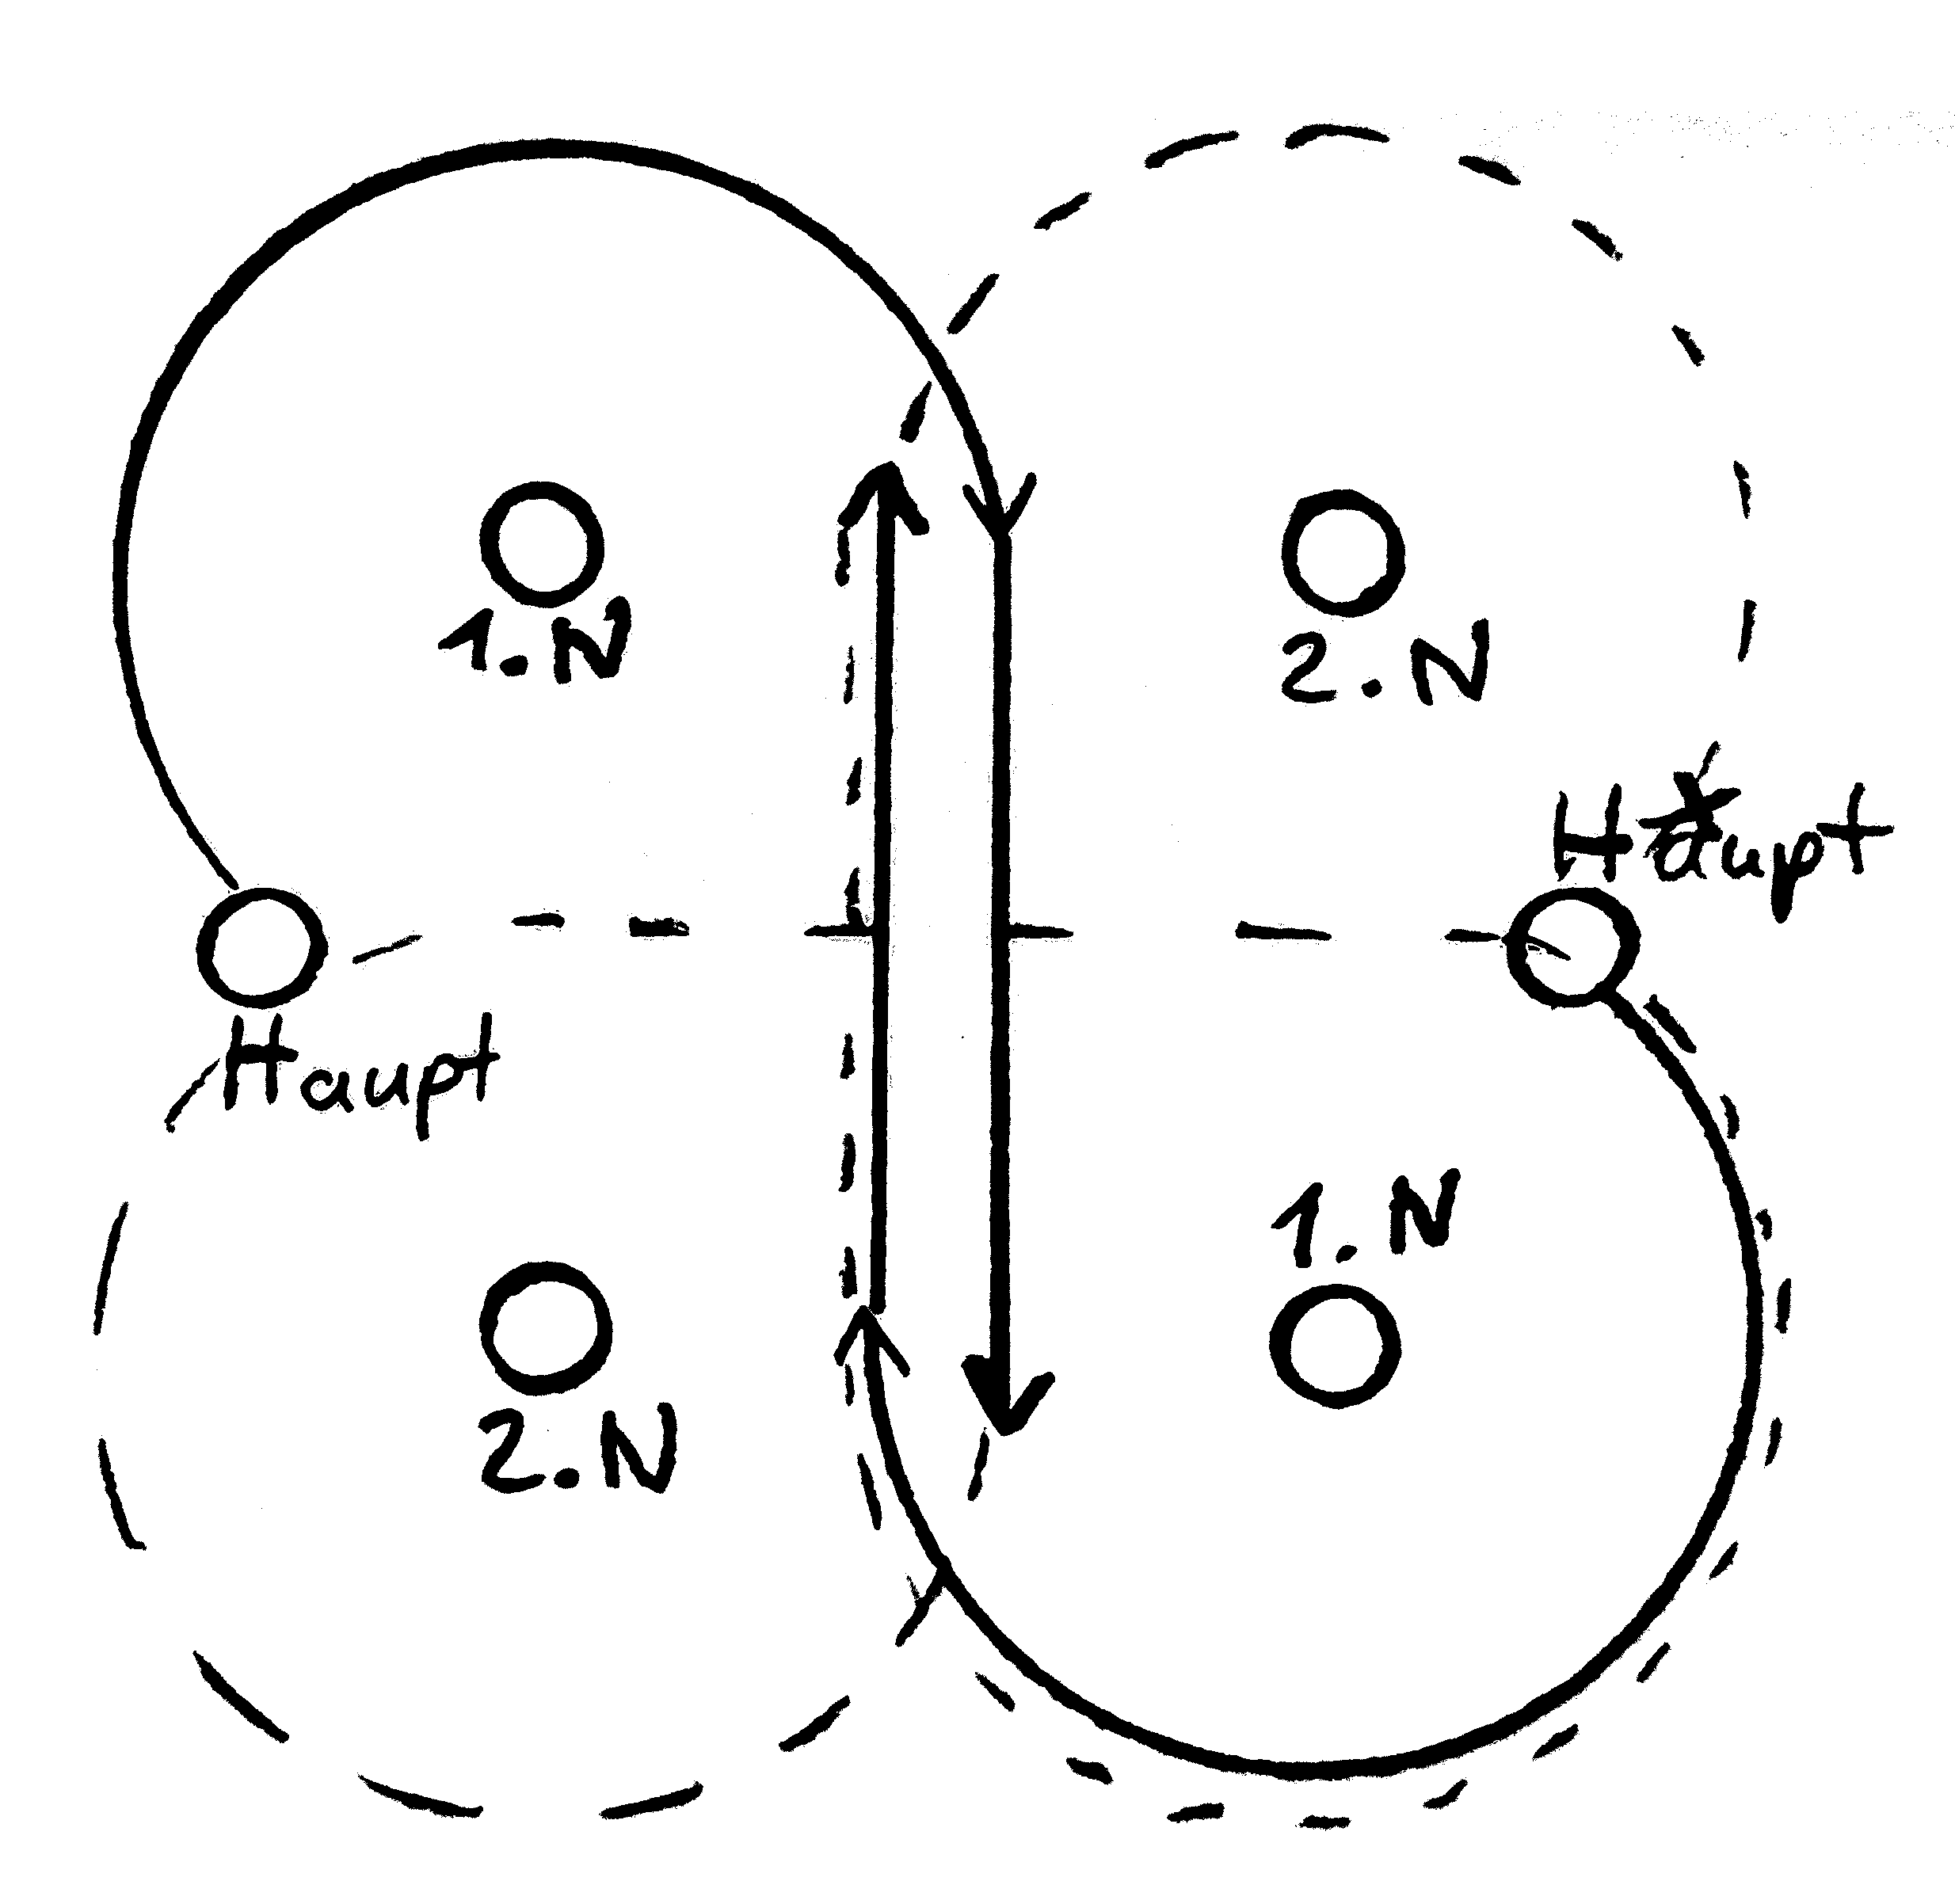
\includegraphics[width=0.5\textwidth]{img/Gingerbread}
\end{center}


%%%%%%%%%%%%%%%%%%%%%%%%%%%%%%%%%%%%%%%%%%%%%%%%%%%%%%%%%%%%%%%%%%%%%%%%%%%%%%%%
% Gotham Jubilee
%%%%%%%%%%%%%%%%%%%%%%%%%%%%%%%%%%%%%%%%%%%%%%%%%%%%%%%%%%%%%%%%%%%%%%%%%%%%%%%%
\newpage

\dancename{Gotham Jubilee}
\iffalse\subsection{Gotham Jubilee}\fi % fool texstudio into displaying subsections
\danceinfo{Longway for as many as will,\\ \nicefrac{6}{8} Takt}
\danceinstructionsbegin
Takte&\\
1 -- 8 	& D2 cast up um D1 in Figure of Eight um D1 und H2, H1 verfolgt bis beide wieder auf der Ausgangsposition ankommen\\
9 -- 16 & H2 cast up um H1 in Figure of Eight... D1 verfolgt ...\\
\danceinstructionsel
1 -- 2 	& Partner rechte Hände, Balance vor und zurück\\
3 -- 4 	& Platzwechsel (Dame dreht unter dem Arm des Herren)\\
5 -- 8 	& Dos-à-dos (langsam)\\
\danceinstructionsel
1 -- 4 	& \nicefrac{1}{2} Pousette im Set, H1 \& D2 schieben\\
5 -- 6 	& linke Hände reichen, Set links\\
7 -- 8 	& Platzwechsel (beliebig)
\dancemediummarker
\danceinstructionsend


%%%%%%%%%%%%%%%%%%%%%%%%%%%%%%%%%%%%%%%%%%%%%%%%%%%%%%%%%%%%%%%%%%%%%%%%%%%%%%%%
% Grimstock
%%%%%%%%%%%%%%%%%%%%%%%%%%%%%%%%%%%%%%%%%%%%%%%%%%%%%%%%%%%%%%%%%%%%%%%%%%%%%%%%
\newpage

\dancename{Grimstock}
\iffalse\subsection{Grimstock}\fi % fool texstudio into displaying subsections
\danceinfo{Longway for three couples}
\danceinstructionsbegin
%\textbf{Strophe}&\textbf{I}\\
1 -- 8 	& Lead up \& down\\
9 -- 16 & Set \& Turn links\\
1 -- 16 	& Wiederholung rechts\\
\danceinstructionsel
\textbf{Refrain}&\\
1 -- 16 & Herren und Damen tanzen auf den Seitenlinien eine Hecke. Dabei startet Paar 1 in die Gassenmitte.\\
\danceinstructionsel
%\textbf{Strophe}&\textbf{II}\\
1 -- 8 	& Siding links\\
9 -- 16 	& Set \& Turn links\\
1 -- 8 	& Wiederholung rechts\\
\danceinstructionsel
\danceinstructionsel
\textbf{Refrain}&\\
1 -- 16 & Wie auch schon vorher. Diesmal bilden die gerade außen gehenden Pärchen Tore, durch die die inneren durchgehen.\\
\danceinstructionsel
%\textbf{Strophe}&\textbf{III}\\
1 -- 8 	& Armtour links\\
9 -- 16 	& Set \& Turn links\\
1 -- 16 & Wiederholung rechts\\
\danceinstructionsel
\textbf{Refrain}&\\
1 -- 16 & Wie auch schon vorher (ohne Tore), Paar 1 kreuzt aber jedes mal, wenn es Paar 2 passiert\\
\danceinstructionsend
\textit{(Keine Wiederholungen)}
\dancedifficultmarker


%%%%%%%%%%%%%%%%%%%%%%%%%%%%%%%%%%%%%%%%%%%%%%%%%%%%%%%%%%%%%%%%%%%%%%%%%%%%%%%%
% Gypsy Girl's Headscarf
%%%%%%%%%%%%%%%%%%%%%%%%%%%%%%%%%%%%%%%%%%%%%%%%%%%%%%%%%%%%%%%%%%%%%%%%%%%%%%%%
\newpage

\dancename{Gypsy Girl's Headscarf}
\origininfo{~}{Häufig Kesh Jig}{z.B The Mountain Laurels}
\iffalse\subsection{Gypsy Girl's Headscarf}\fi % fool texstudio into displaying subsections
\danceinfo{Kreistanz, 8 Tänzer}

\textit{Alle stehen durchgefasst, wie für einen Longway. Der Tanz hat in der Strophe Longwaycharakter. Oben ist dann durch normales ”proper“ zu erkennen.}
\danceinstructionsbegin
1 -- 8 	& Alle hüpfen links herum im Kreis.\\
9 -- 16 & Alle hüpfen rechtsherum zurück.\\
\danceinstructionsel
& \textit{Dame 1 und Herr 1 lösen ihre Hände:}\\
1 -- 16 & Herr 1 und 2 heben die gemeinsamen Hände zu einem Tor. Dame 1 geht hindurch, alle anderen folgen und bilden wieder einen Kreis\\
1 -- 16 & Dame 1 und 2 heben die gemeinsamen Hände zu einem Tor. Herr 1 geht hindurch, alle anderen folgen und bilden \textbf{eine Gasse}!\\ 
\danceinstructionsel
1 -- 4 	& Paar 1 gibt sich beide Hände und hüpft im Seitgalopp die Gasse hinunter\\
5 -- 8 	& Paar 4 legt die Händer auf den Schulter von Paar 1 und galoppiert wieder mit hoch\\
1 -- 8 	& Paar 4 rückt auf Position 1 auf die Tänzer bilden wieder einen Kreis.\\
\danceeasymarker
\danceinstructionsend


%%%%%%%%%%%%%%%%%%%%%%%%%%%%%%%%%%%%%%%%%%%%%%%%%%%%%%%%%%%%%%%%%%%%%%%%%%%%%%%%
% Heart's Ease
%%%%%%%%%%%%%%%%%%%%%%%%%%%%%%%%%%%%%%%%%%%%%%%%%%%%%%%%%%%%%%%%%%%%%%%%%%%%%%%%
\newpage

\dancename{Heart's Ease}
\origininfo{Playford 1651}{Playford}{~}
\iffalse \subsection{Heart's Ease}\fi % fool texstudio into displaying subsections
\danceinfo{Tanz für zwei Paare\\D1~~~H1\\H2~~D2}
\danceinstructionsbegin
\textbf{Strophe} & \textbf{I}\\
1 -- 8 & Paare zueinander Meet \& Fall back\\
9 -- 16 & Wiederholung\\
\danceinstructionsel
\textbf{Refrain}&\\
1 -- 8 & Herren Fallback \& Meet (zur Setmitte gewandt)\\
9 -- 16 & Rechte Handtour der Kontras (Variante: Männer zwischen Meet und Handtour abklatschen)\\
1 -- 8 & Alle Fallback und Turn rechts (zur Setmitte gewandt)\\
9 -- 16 & Linke Handtour der Partner\\
\danceinstructionsel

\textbf{Strophe}& \textbf{II}\\
1 -- 8 & Siding links mit Partner\\
9 -- 16 & Siding rechts mit Kontra\\
\danceinstructionsel
\textbf{Refrain}&\textbf{wiederholen}\\
\danceinstructionsel
\textbf{Strophe}& \textbf{III}\\
1 -- 8 & Armtour links mit Partner\\
9 -- 16 & Armtour rechts mit Kontra\\
\danceinstructionsel
\textbf{Refrain}&\textbf{wiederholen}\\

\dancedifficultmarker
\danceinstructionsend


%%%%%%%%%%%%%%%%%%%%%%%%%%%%%%%%%%%%%%%%%%%%%%%%%%%%%%%%%%%%%%%%%%%%%%%%%%%%%%%%
% Heart's Ease (Saltatio)
%%%%%%%%%%%%%%%%%%%%%%%%%%%%%%%%%%%%%%%%%%%%%%%%%%%%%%%%%%%%%%%%%%%%%%%%%%%%%%%%
\newpage

\dancename{Heart's Ease {\normalsize(Saltatio)}}
\origininfo{Playford 1651, abgewandelt}{Playford}{~}
\iffalse \subsection{Heart's Ease (Saltatio)}\fi % fool texstudio into displaying subsections
\danceinfo{Tanz für zwei Paare\\D1~~~H1\\H2~~D2}
\danceinstructionsbegin
\textbf{Strophe} & \textbf{I}\\
1 -- 8 & Paare zueinander Meet \& Fall back\\
9 -- 16 & Wiederholung\\
\danceinstructionsel
\textbf{Refrain}&\\
1 -- 8 & Fallback \& Meet mit Kontra(also zum Kontra gewendet)\\
9 -- 16 & Rechte Handtour der Kontras\\
1 -- 8 & Fallback \& Meet mit Partner(also zum Partner gewendet)\\
9 -- 16 & Linke Handtour mit Partner\\
\danceinstructionsel
\danceinstructionsel
\danceinstructionsel
\textbf{Strophe} & \textbf{II}\\
1 -- 8 & Siding links mit Partner\\
9 -- 16 & Siding rechts mit Kontra\\
\danceinstructionsel
\textbf{Refrain}&\textbf{wiederholen}\\
\danceinstructionsel
\textbf{Strophe} & \textbf{III}\\
1 -- 8 & Armtour links mit Partner\\
9 -- 16 & Armtour rechts mit Kontra\\
\danceinstructionsel
\textbf{Refrain}&\textbf{wiederholen}\\

\dancedifficultmarker
\danceinstructionsend


%%%%%%%%%%%%%%%%%%%%%%%%%%%%%%%%%%%%%%%%%%%%%%%%%%%%%%%%%%%%%%%%%%%%%%%%%%%%%%%%
% Heptathlon
%%%%%%%%%%%%%%%%%%%%%%%%%%%%%%%%%%%%%%%%%%%%%%%%%%%%%%%%%%%%%%%%%%%%%%%%%%%%%%%%
\newpage

\dancename{Heptathlon}
\iffalse \subsection{Heptathlon}\fi % fool texstudio into displaying subsections
\danceinfo{7 Tänzer, in einem 'H' aufgestellt}
\danceinstructionsbegin
1 -- 8 	& Stern zu dritt oben rechts\\
1 -- 8 	& Stern zu dritt oben links\\
1 -- 8 	& Stern zu dritt unten rechts\\
1 -- 8 	& Stern zu dritt unten links\\
\danceinstructionsel
1 -- 16 & Heckenacht der mittleren Reihe\\
1 -- 8 	& Die Mitte tanzt mit rechts oben 1½ Ronden\\
~		& \textit{bzw. etwas beschwingtes, das in einem Platzwechsel resultiert}\\
1 -- 8 	& Set \& Turn links auf die nächste Außenposition\\
\danceeasymarker
\danceinstructionsend


%%%%%%%%%%%%%%%%%%%%%%%%%%%%%%%%%%%%%%%%%%%%%%%%%%%%%%%%%%%%%%%%%%%%%%%%%%%%%%%%
% Hey Boys Up Go We
%%%%%%%%%%%%%%%%%%%%%%%%%%%%%%%%%%%%%%%%%%%%%%%%%%%%%%%%%%%%%%%%%%%%%%%%%%%%%%%%
\newpage

\dancename{Hey Boys Up Go We}
\iffalse\subsection{Hey Boys Up Go We}\fi % fool texstudio into displaying subsections
\danceinfo{Longway for as many as will}
\danceinstructionsbegin
1 -- 8 	& Paar 1 \& Dame 2 Ronde zu dritt\\
1 -- 8 	& Paar 1 \& Herr 2 Ronde zu dritt\\
1 -- 8 	& Fall back \& meet\\
1 -- 8 	& Dos-à-dos auf der Seitenlinie\\
\danceinstructionsel
1 -- 4 	& Paar 1 klatscht: Eigene Hände, rechte Hände, eigene Hände, linke Hände\\
5 -- 8 	& Paar 1 cast down, Paar 2 lead up\\
\danceinstructionsel
1 -- 4 	& Herr 1 \& 2 klatschen: Eigene Hände, rechte, eigene, linke\\
5 -- 8 	& Dame 1 \& 2 klatschen: Eigene Hände 2x, Beide Hände 2x\\
\dancemediummarker
\danceinstructionsend


%%%%%%%%%%%%%%%%%%%%%%%%%%%%%%%%%%%%%%%%%%%%%%%%%%%%%%%%%%%%%%%%%%%%%%%%%%%%%%%%
% Hole in the Wall
%%%%%%%%%%%%%%%%%%%%%%%%%%%%%%%%%%%%%%%%%%%%%%%%%%%%%%%%%%%%%%%%%%%%%%%%%%%%%%%%
\newpage

\dancename{Hole in the Wall}
\iffalse\subsection{Hole in the Wall}\fi % fool texstudio into displaying subsections
\danceinfo{Longway for as many as will\\¾ Takt, Walzerschritte}
\danceinstructionsbegin
1--12 	& Paar 1 Cast down \& Lead up\\
1--12 	& Paar 2 Cast up \& Lead down\\
~ & ~ \\
1--6 	& FC Platzwechsel rechte Hand, kurz in der Mitte verharren\\
7--12	& SC Platzwechsel linke Hand, kurz in der Mitte verharren\\
~ & ~ \\
1--6 	& Halber Setkreis\\
7--12	& Paar 1 Cast down und zieht Paar 2 hoch \\
\danceeasymarker
\danceinstructionsend


%%%%%%%%%%%%%%%%%%%%%%%%%%%%%%%%%%%%%%%%%%%%%%%%%%%%%%%%%%%%%%%%%%%%%%%%%%%%%%%%
% Hundson House
%%%%%%%%%%%%%%%%%%%%%%%%%%%%%%%%%%%%%%%%%%%%%%%%%%%%%%%%%%%%%%%%%%%%%%%%%%%%%%%%
% \newpage

\iffalse\subsection{[Hundson House]}\fi % fool texstudio into displaying subsections
% \dancename{Hundson House}
% \danceinfo{}
% \danceinstructionsbegin
% \danceinstructionsend
% \dancedifficultmarker


%%%%%%%%%%%%%%%%%%%%%%%%%%%%%%%%%%%%%%%%%%%%%%%%%%%%%%%%%%%%%%%%%%%%%%%%%%%%%%%%
% Hunt the Squirrel
%%%%%%%%%%%%%%%%%%%%%%%%%%%%%%%%%%%%%%%%%%%%%%%%%%%%%%%%%%%%%%%%%%%%%%%%%%%%%%%%
\newpage

\iffalse\subsection{Hunt the Squirrel}\fi % fool texstudio into displaying subsections
\dancename{Hunt the Squirrel}
\origininfo{Playford, abgewandelt}{Playford}{}
\danceinfo{Longway for as many as will}
\danceinstructionsbegin
1 -- 8 & P1 Lead Down \& Cast up\\
9 -- 16 & H1/H2 Lead durch die Damen und Cast zurück\\
17--24 & P2 Lead Up \& Cast down\\
25--32 & D1/D2 Lead durch Herren und Cast zurück\\
\danceinstructionsel
1 -- 8 & FC Setting steps (links) zueinander \& Turn links zurück\\
9 -- 16 & SC Setting steps (links) zueinander \& Turn links zurück\\
\danceinstructionsel
1 -- 4 & Halber Setkreis \\
5 -- 8 & Linien Fall back\\
9 -- 12 & Setting steps aufeinander zu\\
13 -- 16 & Paare halbe Ronde
\dancedifficultmarker
\danceinstructionsend


%%%%%%%%%%%%%%%%%%%%%%%%%%%%%%%%%%%%%%%%%%%%%%%%%%%%%%%%%%%%%%%%%%%%%%%%%%%%%%%%
%	I care not for these Ladies
%%%%%%%%%%%%%%%%%%%%%%%%%%%%%%%%%%%%%%%%%%%%%%%%%%%%%%%%%%%%%%%%%%%%%%%%%%%%%%%%
\newpage

\dancename{I care not for these Ladies}
\iffalse\subsection{I care not for these Ladies}\fi % fool texstudio into displaying subsections
\danceinfo{Kreistanz\\Herr/Dame durchgefasst}
\danceinstructionsbegin
\textbf{Teil} & \textbf{I}\\
1 -- 8 & Gehüpfte Chassés links herum im Kreis\\
9 -- 16 & Gehüpfte Chassés rechts herum zurück\\
1 -- 8 & Set \& Turn links mit dem Partner\\
\danceinstructionsel
\textbf{Refrain:} & (bzw. Fortschritt)\\
1 -- 4 & Halbe rechte Handtour mit dem Partner\\
5 -- 8 & dann weiter auf Kreisbahn mit dem entgegenkommenden neuen Partner eine halbe linke Handtour\\
9 -- 16 & Mit dem nun entgegenkommenden Partner eine anderthalbe Ronde, sodass man wieder richtig im Kreis steht.\\
\danceinstructionsel
\textbf{Teil} & \textbf{II}\\
1 -- 8 & Die neuen Paare Siding links\\
9 -- 16 & Siding rechts \\
1 -- 8 & Set \& Turn links (manchmal auch rechts für den Ausgleich)\\
\danceinstructionsel
\textbf{Refrain} & \textbf{wiederholen}\\
\danceinstructionsel
\textbf{Teil} & \textbf{III}\\
1 -- 8 & Die neuen Paare Linke Armtour (alternativ Arme einhaken)\\
9 -- 16 & Rechte Armtour (oder Alternative)\\
1 -- 8 & Set \& Turn links\\

\danceinstructionsel
\textbf{Refrain} & \textbf{wiederholen}
\danceeasymarker
\danceinstructionsend


%%%%%%%%%%%%%%%%%%%%%%%%%%%%%%%%%%%%%%%%%%%%%%%%%%%%%%%%%%%%%%%%%%%%%%%%%%%%%%%%
%	Impropriety
%%%%%%%%%%%%%%%%%%%%%%%%%%%%%%%%%%%%%%%%%%%%%%%%%%%%%%%%%%%%%%%%%%%%%%%%%%%%%%%%
\newpage

\dancename{Impropriety}
\origininfo{Brooke Friendly \& Chris Sackett (1999)}{Millisons Jegge}{Playford}
\iffalse\subsection{Impropriety}\fi % fool texstudio into displaying subsections
\danceinfo{Longway, Duple Minor}

\danceinstructionsbegin
1 -- 8 & P2 gatet P1 1\nicefrac{1}{4} Drehungen nach unten.\\
9 -- 16 & Line of Four: Lead down and Fall back up.\\
\danceinstructionsel
1 -- 4 & Linien nach außen schauend ein Double nach außen\\
5 -- 8 & Platzwechsel der 1er und 2er. 2er drehen unter dem Arm der 1er durch und enden mit Blick nach innen.\\
9 -- 12 & Linien wieder ein Double nach innen.\\
\danceinstructionsel
13 -- 16 & P1 cast down, P2 lead up.\\
1 -- 8 & P1 Half figure Eight durch P2.\\
9 -- 16 & P2 gatet P1 einmal nach oben.\\
\dancedifficultmarker
\danceinstructionsend


%%%%%%%%%%%%%%%%%%%%%%%%%%%%%%%%%%%%%%%%%%%%%%%%%%%%%%%%%%%%%%%%%%%%%%%%%%%%%%%%
%	Indian Queen
%%%%%%%%%%%%%%%%%%%%%%%%%%%%%%%%%%%%%%%%%%%%%%%%%%%%%%%%%%%%%%%%%%%%%%%%%%%%%%%%
\newpage

\dancename{Indian Queen}
\iffalse\subsection{Indian Queen}\fi % fool texstudio into displaying subsections
\danceinfo{Longway for as many as will}

\danceinstructionsbegin
1 -- 4  & First Corner Set zum Partner dann zum Kontra\\
5 -- 8  & First Corner Turn rechts\\
9 -- 16 & First Corner Ronde\\
1 -- 8  & Second Corner Set \& Turn zum Partner, dann Kontra\\
9 -- 16 & Second Corner Ronde\\
\danceinstructionsel
1 -- 8  & Mühle rechts herum (rechte Hände) auf 8 Klatschen\\
9 -- 16 & Mühle links herum zurück, auf 8 Klatschen\\
\danceinstructionsel
1 -- 8  & Dos-à-dos\\
1 -- 8  & $\nicefrac{3}{4}$ Kette\\
\danceeasymarker
\danceinstructionsend


%%%%%%%%%%%%%%%%%%%%%%%%%%%%%%%%%%%%%%%%%%%%%%%%%%%%%%%%%%%%%%%%%%%%%%%%%%%%%%%%
% Jamaica
%%%%%%%%%%%%%%%%%%%%%%%%%%%%%%%%%%%%%%%%%%%%%%%%%%%%%%%%%%%%%%%%%%%%%%%%%%%%%%%%
\newpage

\dancename{Jamaica}
\iffalse\subsection{Jamaica}\fi % fool texstudio into displaying subsections
\danceinfo{Longway, Doppelter Fortschritt}
\danceinstructionsbegin
\textbf{I}& \\
1--4 	& P1 „Rechte Hand und linke Hand“(geben)\\
5--8 	& P1 „Auf die andere Seite“ (Platzwechsel)\\
9--16 	& H1+D2 / H2+D1 „Rechte Hand und linke Hand“ + Platzwechsel\\
%\danceinstructionsel
1--12 	& P1 Figure of Eight um P2 \\
13--16	& P1 halbe Ronde (ergibt sich aus Figure of Eight)\\
& \textit{Erster Fortschritt (Es gibt neue Sets)}\\
\textbf{II} & \\
1--8 	& FC Ronde\\
9--16	& SC Ronde\\
1--8 	& H1+H2, D1+D2  1½ Ronde\\
9--16 	& Dos-á-Dos
\dancemediummarker
\danceinstructionsend


%%%%%%%%%%%%%%%%%%%%%%%%%%%%%%%%%%%%%%%%%%%%%%%%%%%%%%%%%%%%%%%%%%%%%%%%%%%%%%%%
% Jenny Pluck Pears
%%%%%%%%%%%%%%%%%%%%%%%%%%%%%%%%%%%%%%%%%%%%%%%%%%%%%%%%%%%%%%%%%%%%%%%%%%%%%%%%
\newpage

\dancename{Jenny Pluck Pears}
\iffalse\subsection{Jenny Pluck Pears}\fi % fool texstudio into displaying subsections
\danceinfo{Kreistanz, 3 Paare, durchgefasst}
\danceinstructionsbegin
\textbf{Strophe}&\textbf{I}\\
1 -- 8 	& Acht Schritte nach links gehen\\
9 -- 16 & Jeder ein Set \& Turn links\\
1 -- 8 	& Acht Schritte nach rechts gehen\\
9 -- 16 & Jeder ein Set \& Turn rechts\\
\danceinstructionsel
\textbf{Refrain}&\textbf{(Herren Dominant)}\\
1 -- 4 	& Herr 1 dreht seine Dame an der rechten Hand in den Kreis\\
5 -- 8 	& Herr 2 ebenso\\
9 -- 12 & Herr 3 ebenso\\
13 -- 16& Alle eine Referenz\\
1 -- 8 	& Die Herren gehen 8 Schritte vor den Damen nach links\\
9 -- 16 & Die Herren tanzen ein Set \& Turn links\\
1 -- 8 	& Die Herren gehen 8 Schritte vor den Damen nach rechts\\
9 -- 16 & Die Herren tanzen ein Set \& Turn rechts\\
1 -- 16 & Herr 1 - 3 dreht seine Dame aus der Mitte \& Referenz\\
\danceinstructionsel
\textbf{Strophe}&\textbf{II}\\
1 -- 8 	& Paare Siding links\\
9 -- 16 & Set \& Turn links\\
1 -- 8 	& Paare Siding rechts\\
9 -- 16 & Set \& Turn rechts\\
\danceinstructionsel
\textbf{Refrain}&\textbf{(Damen Dominant)}\\
&\textit{ergo ersetze Dame mit Herr und andersherum}\\
\danceinstructionsel
\danceinstructionsel
\textbf{Strophe}&\textbf{III}\\
1 -- 8 	& Paare Armtour links\\
9 -- 16 & Set \& Turn links\\
1 -- 8 	& Paare Armtour rechts\\
9 -- 16 & Set \& Turn rechts\\
\danceinstructionsel
\textbf{Refrain}&\textbf{(Herren Dominant)}\\
\dancemediummarker
\danceinstructionsend


%%%%%%%%%%%%%%%%%%%%%%%%%%%%%%%%%%%%%%%%%%%%%%%%%%%%%%%%%%%%%%%%%%%%%%%%%%%%%%%%
% John Tallis' Canon
%%%%%%%%%%%%%%%%%%%%%%%%%%%%%%%%%%%%%%%%%%%%%%%%%%%%%%%%%%%%%%%%%%%%%%%%%%%%%%%%
\newpage

\dancename{John Tallis' Canon}
\origininfo{Pat Shaw}{John Tallis' Canon}{von Pat Shaw}
\iffalse\subsection{John Tallis' Canon}\fi % fool texstudio into displaying subsections
\danceinfo{Longway, Duple minor, Kanon}
%\danceinstructionsbegin
%\dancedifficultmarker
\begin{longtable}{c | c | c}
\textbf{Schläge} & \textbf{First Corner} & \textbf{Second Corner}\\\hline
4 & Meet &  Warten\\
4 & Fall Back  & Meet\\
4 & Platzwechsel & Fall Back\\
4 & Turn links & Platzwechsel\\
4 & Meet & Turn links\\
4 & Fall Back & Meet\\
4 & Platzwechsel & Fall Back\\
4 & Turn single left & Platzwechsel\\
4 & ½ Handtour rechts & Turn single left\\
4 & ½ Mühle rechts & ½ Mühle rechts\\
4 & Setting Steps rückwärts & ½ Handtour rechts\\
4 & Turn zurück auf den Platz & Setting Steps rückwärts\\
4 & ½ Handtour links & Turn zurück auf den Platz\\
4 & ½ Mühle links & ½ Mühle links\\
4 & Double rückwärts & ½ Handtour links\\
4 & Double nach schräg rechts vor & Double rückwärts\\\cline{2-2}
4 & Meet neue Dame... & Double nach schräg links vor\\\cline{3-3}
4 & Fall Back & Meet neue Dame...\\
4 & $\vdots$ & $\vdots$\\
\danceinstructionsend
\textit{Es hilft sich vor dem Start des Tanzes einzuprägen in welche Richtung einen der eigene Fortschritt bringt.}
\dancedifficultmarker


%%%%%%%%%%%%%%%%%%%%%%%%%%%%%%%%%%%%%%%%%%%%%%%%%%%%%%%%%%%%%%%%%%%%%%%%%%%%%%%%
% Juice of Barley (Variante)
% Erläuterungen: abgewandelt,
% Notes:
% Used in the 1996 Television production of Emma.

% Original: 
% The Juice of Barley	Dancing Master 1688
% The 1 cu go back to back with their Partners, and the 2 cu do the same at the same time.
% The 1 cu take hands with his Partner and turn her round, the 2 cu doing the same at the same time.
% The two we stand still, whilst the 1 man goes round about the 2 wo into the 2 man’s place, and the 2 man goes round about the 1 wo into the 1 man’s place, 
% then all clap hands, then all four take hands and go quite round, the we doing the like. 
%%%%%%%%%%%%%%%%%%%%%%%%%%%%%%%%%%%%%%%%%%%%%%%%%%%%%%%%%%%%%%%%%%%%%%%%%%%%%%%%
\newpage

\dancename{Juice of Barley \normalsize{(Variante)}}
\iffalse\subsection{Juice of Barley (Variante)}\fi % fool texstudio into displaying subsections
\origininfo{Playford abgewandelt}{Playford}{}
\danceinfo{Longway for as many as will}
\danceinstructionsbegin
1 -- 8 &	Paare Dos-á-Dos \\
		& umrunden + vertreiben\\
1 -- 8 &	H1 durch Damen, um D2 auf Platz H2 \\
9 -- 16 &	H2 durch Damen, um D1 auf Platz H1 \\
1 -- 8 &	D1 durch Herren, um H1 auf Platz D2 \\
9 -- 16 &	D2 durch Herren, um H2 auf Platz D1 \\
1 -- 4 &	P1 geht gefasst nach oben (verabschieden)\\
5 -- 8 & 	und wieder zurück\\
\dancemediummarker
\danceinstructionsend


%%%%%%%%%%%%%%%%%%%%%%%%%%%%%%%%%%%%%%%%%%%%%%%%%%%%%%%%%%%%%%%%%%%%%%%%%%%%%%%%
% Juice of Barley (Playford)
%%%%%%%%%%%%%%%%%%%%%%%%%%%%%%%%%%%%%%%%%%%%%%%%%%%%%%%%%%%%%%%%%%%%%%%%%%%%%%%%
\newpage

\dancename{Juice of Barley \normalsize{(Playford)}}
\iffalse\subsection{Juice of Barley (Playford)}\fi % fool texstudio into displaying subsections
\origininfo{Playford}{Playford}{}
\danceinfo{Longway for as many as will}
\danceinstructionsbegin
1 -- 8 &	Paare Dos-á-Dos \\
9 -- 16 & 	Paare Ronde \\
1 -- 8 & 	H1 \& H2 Half-Figure-Eight durch die Damen auf des jeweils anderen Platz\\
9 -- 16 & 	Klatschen auf den ersten Schlag, dann Setkreis ganz herum\\
1 -- 8 & 	D1 \& D2 Half-Figure-Eight durch die Herren auf des jeweils anderen Platz\\
9 -- 16 & 	Klatschen auf den ersten Schlag, dann Setkreis ganz herum\\
\danceeasymarker
\danceinstructionsend


%%%%%%%%%%%%%%%%%%%%%%%%%%%%%%%%%%%%%%%%%%%%%%%%%%%%%%%%%%%%%%%%%%%%%%%%%%%%%%%%
% Key to the Cellar
%%%%%%%%%%%%%%%%%%%%%%%%%%%%%%%%%%%%%%%%%%%%%%%%%%%%%%%%%%%%%%%%%%%%%%%%%%%%%%%%
\newpage

\dancename{Key to the Cellar}
\iffalse\subsection{Key to the Cellar}\fi % fool texstudio into displaying subsections
\danceinfo{Triple Minor Longway, Paar 1 improper}
\danceinstructionsbegin
1 -- 6 	& Paar 1 auswenden auf Pos 2, Paar 2 aufrücken\\
7 -- 12 & P3 gatet P1\\
1 -- 6 	& Fallback \& Meet\\
7 -- 12	& P2 gatet P1\\
1 -- 12 & 1er gehn nach links in eine verwobene Figure of Eight\\
1 -- 6 	& \textit{Longway:} \\
& Paar 1 Ronde\\
& \textit{3 Paare:}\\
& Paar 1 rondiert auf Pos 3. \\
& Paar 3 wendet aus auf Pos. 2\\
7 -- 12 & Alle Ronde\\
\dancemediummarker
\danceinstructionsend


%%%%%%%%%%%%%%%%%%%%%%%%%%%%%%%%%%%%%%%%%%%%%%%%%%%%%%%%%%%%%%%%%%%%%%%%%%%%%%%%
%	Korobushka (Gasse)
%%%%%%%%%%%%%%%%%%%%%%%%%%%%%%%%%%%%%%%%%%%%%%%%%%%%%%%%%%%%%%%%%%%%%%%%%%%%%%%%
\newpage

\dancename{Korobushka (Gasse)}
\iffalse\subsection{Korobushka (Gasse)}\fi % fool texstudio into displaying subsections
\danceinfo{Longway for as many as will\\(ohne Fortschritt)}
%\dancemediummarker
\textit{\footnotesize Korobushka-Fassung: die Paare geben sich jeweils die rechten und linken Hände und halten diese gekreuzt.}\\
Paare in Korobushka-Fassung nach oben schauend.
\danceinstructionsbegin
1 -- 4  & Double vor (letzter Tap)\\
5 -- 8  & Double zurück (letzter Tap)\\
9 -- 16 & Wiederholen, am Ende zueinander drehen (ohne Fassung zu lösen)\\
1 -- 2  & Zueinander hüpfen\\
3 -- 4 	& Auseinander hüpfen\\
5 -- 8  & Nocheinmal Zueinander \& auseinander\\
9 -- 12  & Platzwechsel (danach Hände loslassen)\\
13 -- 16 & Dreimal Stampfen und Klatschen (16 ohne Klatschen)\\
1 -- 4 & Nach links mit rechts kreuzen nach links und Kick\\
5 -- 8 & Nach rechts mit links kreuzen nach rechts und Kick\\
9 -- 12 & (Korobushkafassung) Zueinander \& Auseinander\\
13 -- 16 & Platzwechsel
\dancemediummarker
\danceinstructionsend


%%%%%%%%%%%%%%%%%%%%%%%%%%%%%%%%%%%%%%%%%%%%%%%%%%%%%%%%%%%%%%%%%%%%%%%%%%%%%%%%
%	Korobushka (Kreis)
%%%%%%%%%%%%%%%%%%%%%%%%%%%%%%%%%%%%%%%%%%%%%%%%%%%%%%%%%%%%%%%%%%%%%%%%%%%%%%%%
\newpage

\dancename{Korobushka (Kreis)}
\iffalse\subsection{Korobushka (Kreis)}\fi % fool texstudio into displaying subsections
\danceinfo{Kreistanz, Paare schauen sich an, Herr innen}
%\dancemediummarker
\danceinstructionsbegin
1 -- 4  & Paar Doppel nach außen, letzter Schritt Tap. Herr mit links los, Dame mit rechts.\\
5 -- 8  & Double zurück (Tap)\\
9 -- 12 & Doppel vor (Tap)\\
13 -- 16 & Hüpfen mit links, rechter Fuß: vorwärts, seitwärts, ran\\
1 -- 4  & nach links zum nächsten Partner drehen und klatschen (abstoßen)\\
5 -- 8  & zurückdrehen und klatschen.\\
9 -- 12 & rechte Hände geben, zueinander \& auseinander hüpfen\\
13 -- 16 & Platztausch, Dame dreht unter Herr durch\\
1 -- 8 & Nach links drehen, klatschen, zurück und klatschen\\
9 -- 12 & rechte Hände geben, zueinander \& auseinander hüpfen\\
13 -- 16 & Der Herr dreht die Dame unter seinem Arm nach rechts, sodass sie außen steht und geht selbst nach links innen in den Kreis
\dancemediummarker
\danceinstructionsend


%%%%%%%%%%%%%%%%%%%%%%%%%%%%%%%%%%%%%%%%%%%%%%%%%%%%%%%%%%%%%%%%%%%%%%%%%%%%%%%%
% Land of Mist and Wonder
%%%%%%%%%%%%%%%%%%%%%%%%%%%%%%%%%%%%%%%%%%%%%%%%%%%%%%%%%%%%%%%%%%%%%%%%%%%%%%%%
\newpage

\dancename{Land of Mist and Wonder}
\origininfo{Gary Roodman (2018)}{Mylne's Court}{von Rachel Bell}
\iffalse\subsection{Land of Mist and Wonder}\fi % fool texstudio into displaying subsections
\danceinfo{4-Paar Set, 1er und 3er improper,\\ 2er und 3er stehen Rücken an Rücken, ¾-Takt}
\danceinstructionsbegin
\textbf{Teil}&\textbf{A1:}\\
1 -- 8 \footnotesize{(Takte)}	& Mirror-image-Hey auf den Seitenlinien. Die 1er gehen durch die 2er, die 3er gehen durch die 4er. Drei Schritte für jeden Wechsel. Die Paare können wann immer möglich Handfassung aufnehmen.\\
\textbf{Teil}& \textbf{A2:}\\
1 -- 4 & 1er lead down durch die anderen Paare, turn single und lead up\\
5 -- 8 & Invert Lines: Die 1er casten auf die Position der 4er. Die anderen Paare folgen ihnen, so dass am Ende die 1er mit den 4ern und die 2er mit den 3ern die Plätze getauscht haben.\\
&\\
\textbf{Teil} & \textbf{B:}\\
1 -- 4 	& Vor dem Partner Set and turn single\\
5 -- 6 	& Halber Rechthandstern auf den Positionen 1 und 2 sowie auf Positionen 3 und 4\\
7 -- 8 	& Halber Linkhandstern auf Positionen 2 und 3\\
9 -- 12 & In den Sets Positionen 1 und 2 sowie 3 und 4) mit Nachbarn auf der Seitenlinie 1 1/2 Rechthandronden\\
13--14 	& In den Sets durchfassen zum Viererkreis und halb herum im Uhrzeigersinn\\
15--16  & Pause: Gut, um sich für die Mirror-Hecke auszurichten. Sonst z.B. Turn rechts
\dancedifficultmarker
\danceinstructionsend


%%%%%%%%%%%%%%%%%%%%%%%%%%%%%%%%%%%%%%%%%%%%%%%%%%%%%%%%%%%%%%%%%%%%%%%%%%%%%%%%
% La Matelotte
% Info:
% from Feuillets 1706: "Recueil de contredances mises en chorégraphie d'une manière si aisée que toutes personnes peuvent facilement les apprendre"
% Dance can be found on Book pages 121 - 128
% Music: 
%  - Taken from Marin Marais Opera Alcione (or Alcyone) in Act III Scene 2/3
%    -> Not practical for dancing since it would have to be cut first.
%  Available "dancable" music:
%  - Artist: Les Talens Lyriques / Christophe Rousset
%    - Album: Musiques à danser à la cour et à l'opéra
%      - Title: Alcyone ; La Matelotte
%  - Amazon: https://www.amazon.fr/Musiques-%C3%A0-Danser-Cour-lOp%C3%A9ra/dp/B000001Z2T
%  - https://www.youtube.com/watch?v=g-e-5VSgpvY
%%%%%%%%%%%%%%%%%%%%%%%%%%%%%%%%%%%%%%%%%%%%%%%%%%%%%%%%%%%%%%%%%%%%%%%%%%%%%%%%
\newpage

\iffalse\subsection{La Matelotte}\fi % fool texstudio into displaying subsections
\origininfo{Feuillet (1706)}{La Matelote (Thema aus Alcione)}{Marin Marais}
\dancename{La Matelotte}
\danceinfo{Longway, Duple Minor}
\danceinstructionsbegin
1 -- 8 & P1 Lead up \& Cast Down durch P2 des oberen Sets\\
1 -- 8 & P1 Lead down \& Cast Up durch P2\\
1 -- 8 & P1 Half figure eight durch P2\\
1 -- 8 & P1 Ronde\\
1 -- 8 & Dosado auf Linien\\
1 -- 8 & Ronde auf Linien\\
1 -- 8 & P1 Dosado.\\
1 -- 8 & P1 halbe Ronde \& Cast Down, P2 Lead up\\
\dancemediummarker
\danceinstructionsend


%%%%%%%%%%%%%%%%%%%%%%%%%%%%%%%%%%%%%%%%%%%%%%%%%%%%%%%%%%%%%%%%%%%%%%%%%%%%%%%%
% Lillibulero
% There are a lot of versions of this dance.
% This one is from the original Playford Book: 
% http://playforddances.com/dances/lilli-burlero/
%%%%%%%%%%%%%%%%%%%%%%%%%%%%%%%%%%%%%%%%%%%%%%%%%%%%%%%%%%%%%%%%%%%%%%%%%%%%%%%%
\newpage

\iffalse\subsection{Lilli Burlero (Playford)}\fi % fool texstudio into displaying subsections
\dancename{Lilli Burlero {\normalsize(Playford)}}
\origininfo{Playford (???)}{???}{}
\danceinfo{Longway, Duple Minor}
\danceinstructionsbegin
1 -- 8 & Paar 1 Lead Down \& Cast Up\\
1 -- 8 & Paar 2 Lead Up \& Cast Down\\
1 -- 4 & First Corner Platzwechsel\\
5 -- 8 & Second Corner Platzwechsel\\
\danceinstructionsel
1 -- 4 & Seitenlinien fassen im Set durch, Balance zurück und wieder nach vorne\\
5 -- 8 & Partner passieren sich und Turn Single\\
1 -- 8 & Dos-a-dos auf der Linie\\
1 -- 8 & \nicefrac{3}{4} Kette auf der Seitenlinie beginnend\\
\dancemediummarker
\danceinstructionsend

%%%%%%%%%%%%%%%%%%%%%%%%%%%%%%%%%%%%%%%%%%%%%%%%%%%%%%%%%%%%%%%%%%%%%%%%%%%%%%%%
% Lillibulero
% Modern version seen in many places. For example:
% https://www.youtube.com/watch?v=ebJYcPEPE-Y
%%%%%%%%%%%%%%%%%%%%%%%%%%%%%%%%%%%%%%%%%%%%%%%%%%%%%%%%%%%%%%%%%%%%%%%%%%%%%%%%
\newpage

\iffalse\subsection{Lilli Burlero (Modern)}\fi % fool texstudio into displaying subsections
\dancename{Lilli Burlero {\normalsize(Modern)}}
\danceinfo{Longway, Duple Minor}
\danceinstructionsbegin
1 -- 8 & Paar 1 Lead Down \& Cast Up\\
1 -- 8 & Paar 2 Lead Up \& Cast Down\\
1 -- 4 & First Corner Platzwechsel\\
5 -- 8 & Second Corner Platzwechsel\\
\danceinstructionsel
1 -- 4 & Seitenlinien fassen im Set durch, 4 Schritte Fall back\\
5 -- 8 & Turn Single auf Grundlinie und Passieren\\
1 -- 8 & Dos-a-dos auf der Linie\\
1 -- 8 & \nicefrac{4}{4} Kette auf der Seitenlinie beginnend\\
\dancemediummarker
\danceinstructionsend

%%%%%%%%%%%%%%%%%%%%%%%%%%%%%%%%%%%%%%%%%%%%%%%%%%%%%%%%%%%%%%%%%%%%%%%%%%%%%%%%
% Lillibulero
% Modern version seen in many places. Mostly seen in the US.
%%%%%%%%%%%%%%%%%%%%%%%%%%%%%%%%%%%%%%%%%%%%%%%%%%%%%%%%%%%%%%%%%%%%%%%%%%%%%%%%
\newpage

\iffalse\subsection{Lilli Burlero (1/2 Dos-a-dos)}\fi % fool texstudio into displaying subsections
\dancename{Lilli Burlero {\normalsize(\nicefrac{1}{2} Dos-a-dos)}}
\danceinfo{Longway, Duple Minor}
\danceinstructionsbegin
1 -- 8 & Paar 1 Lead Down \& Cast Up\\
1 -- 8 & Paar 2 Lead Up \& Cast Down\\
1 -- 4 & First Corner Platzwechsel\\
5 -- 8 & Second Corner Platzwechsel\\
\danceinstructionsel
1 -- 4 & Seitenlinien fassen im Set durch, 4 Schritte Fall back\\
5 -- 8 & Turn Single auf Grundlinie\\
1 -- 4 & Passieren der Partner \\
5 -- 8 & „Halbes Dos-a-dos“ = Passieren auf der Seitenlinie während man rückwärts geht (Letzter Teil eines Dos-a-dos).\\
1 -- 8 & \nicefrac{4}{4} Kette auf der Seitenlinie beginnend\\
\dancemediummarker
\danceinstructionsend

%%%%%%%%%%%%%%%%%%%%%%%%%%%%%%%%%%%%%%%%%%%%%%%%%%%%%%%%%%%%%%%%%%%%%%%%%%%%%%%%
% Lulle Me Beyond Thee
%%%%%%%%%%%%%%%%%%%%%%%%%%%%%%%%%%%%%%%%%%%%%%%%%%%%%%%%%%%%%%%%%%%%%%%%%%%%%%%%
\newpage

\iffalse\subsection{Lulle Me Beyond Thee}\fi % fool texstudio into displaying subsections
\dancename{Lulle Me Beyond Thee}
\origininfo{Playford (1651)}{Playford}{}
\danceinfo{Playford für Vier Paare, Aufstellung:\\H~~H~~D~~D\\[-0.1cm]D~~D~~H~~H}
% Hacking a bit to get enough space for the attribution at the bottom
\vspace{-.3cm}
\danceinstructionsbegin
\textbf{Strophe} & \textbf{I} \\
1 -- 8 & Lead \& Fall Back ~~~(\textit{Linien durchgefasst zueinander})\\
9 -- 16 & Wiederholen \\
\textbf{Umbau}& \textbf{I} \\
1 -- 4 & Die momentan äußeren Paare führen auf die Plätze der inneren Paare. Die inneren Kontrapartner führen nach außen. Neue Linie um 90° gedreht. \\
5 -- 12 & Fall Back \& Lead ~~~(\textit{Linien durchgefasst zueinander}) \\
13 -- 16 & Ganze Ronde (schnell) \\
\textbf{Umbau}& \textbf{II} \\
17--32 & Wiederholen \\

\danceinstructionsel
\danceinstructionsel
\danceinstructionsel
\textbf{Strophe} & \textbf{II} \\
1 -- 8 & Siding links \\
9 -- 16 & Siding rechts, aber Innere siden mit Kontrapartner auf Linie \\
\textbf{Umbau} & \textbf{III} \\
1 -- 4 & Fall Back ~~~(\textit{Linien durchgefasst zueinander})\\
5 -- 8 & Äußere Tänzer klappen in den entstandenen Raum ein. Es entstehen zwei Viererkreise. \\
9 -- 16 & Beide Kreise ganz herum \\
\textbf{Umbau} & \textbf{IV} \\
17--32 & Wiederholen \\
\danceinstructionsel
\danceinstructionsel


\textbf{Strophe} & \textbf{III} \\
1 -- 8 & Armtour links \\
9 -- 16 & Armtour rechts, aber Innere touren mit Kontrapartner auf Linie \\
\textbf{Umbau} & \textbf{V} \\
1 -- 4 & Die momentan äußeren Paare führen auf die Plätze der inneren Paare. Die inneren Kontrapartner führen nach außen. Neue Linie um 90° gedreht. \\
5 -- 8 & Die äußeren Partner bilden Toore (mit der äußeren Hand) und gehen auf die inneren Plätze, die inneren Partner gehen gefasst durch das Tor auf die äußeren Plätze \\
9 -- 16 & Ganze Ronde der Partner \\
\textbf{Umbau} & \textbf{VI} \\
17--32 & Wiederholen\\


\multicolumn{2}{c}{\textbf{\large Umbau I \& II:}}\\
\begin{center}
	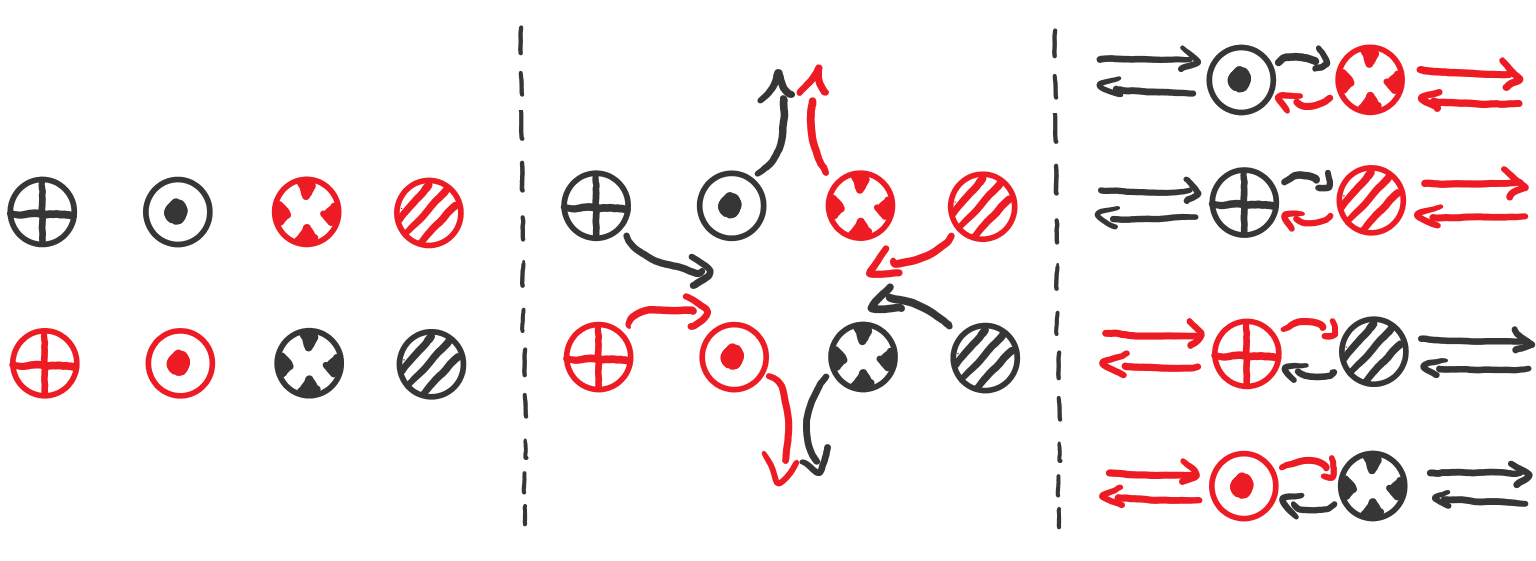
\includegraphics[width=.93\textwidth]{img/lmbt-1}
\end{center}
\danceinstructionsel
\danceinstructionsel
\multicolumn{2}{c}{\textbf{\large Umbau III \& IV:}}\\
\begin{center}
	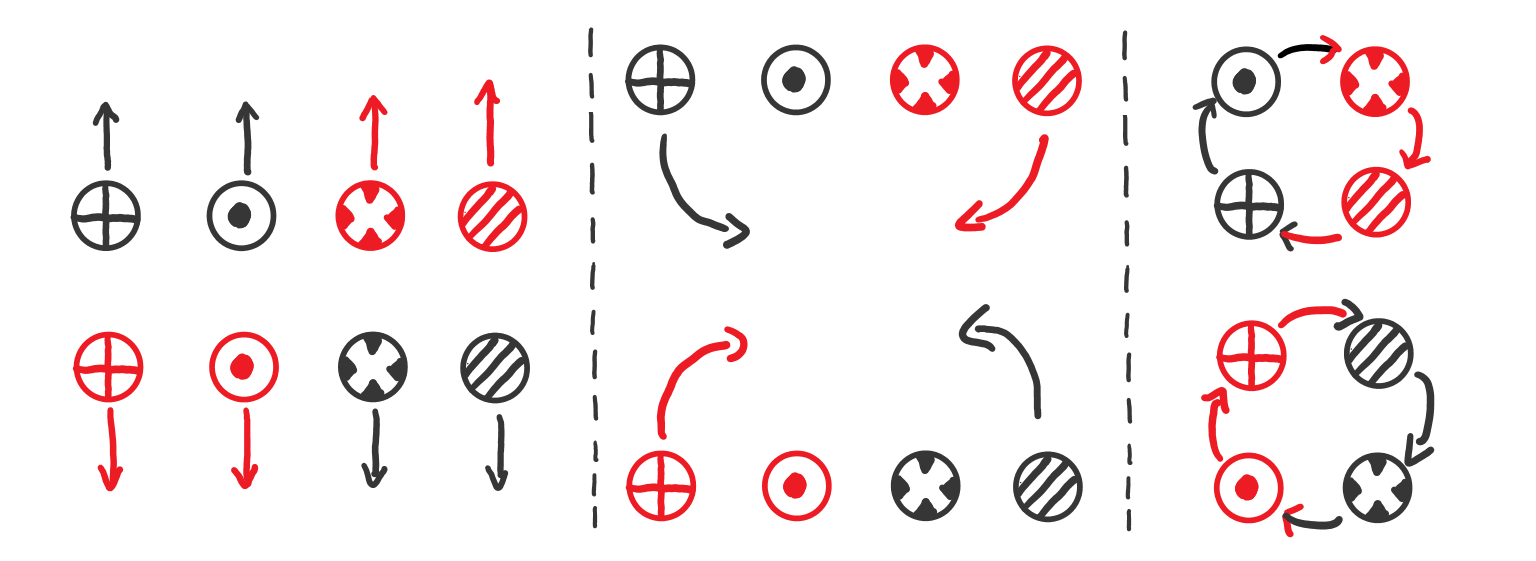
\includegraphics[width=.93\textwidth]{img/lmbt-2}
\end{center}
\danceinstructionsel
\danceinstructionsel

\multicolumn{2}{c}{\textbf{\large Umbau V \& VI:}}\\
\begin{center}
	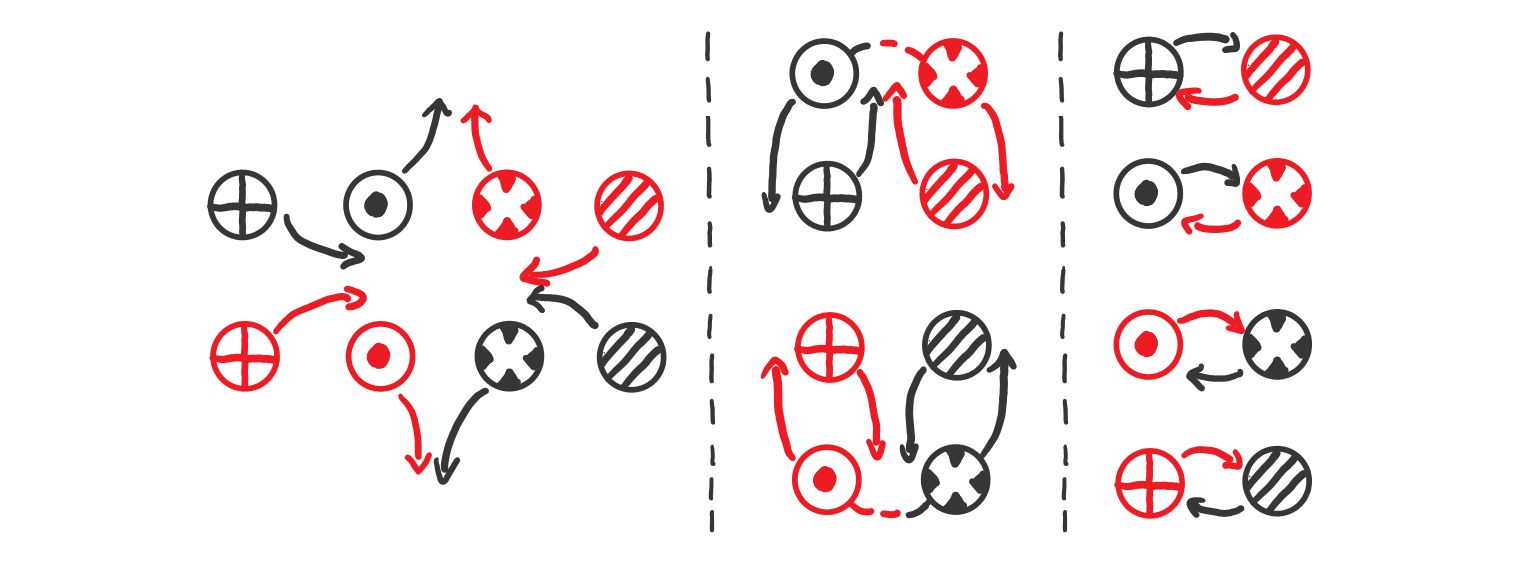
\includegraphics[width=.93\textwidth]{img/lmbt-3}
\end{center}
\dancedifficultmarker
\danceinstructionsend


%%%%%%%%%%%%%%%%%%%%%%%%%%%%%%%%%%%%%%%%%%%%%%%%%%%%%%%%%%%%%%%%%%%%%%%%%%%%%%%%
% Mad Robin
%%%%%%%%%%%%%%%%%%%%%%%%%%%%%%%%%%%%%%%%%%%%%%%%%%%%%%%%%%%%%%%%%%%%%%%%%%%%%%%%
\newpage

\dancename{Mad Robin}
\origininfo{Playford (1695)}{Mad Robin}{Playford}
\iffalse\subsection{Mad Robin}\fi % fool texstudio into displaying subsections
\danceinfo{Longway for as many as will}
\danceinstructionsbegin
1 -- 8 	& First Corner rechte Handtour\\
9 -- 16 & Paar 1 linke Handtour, am Ende Platztausch der Herren\\
1 -- 8 	& Paar 1 linke Handtour\\
9 -- 16 & D1 + H2 rechte Handtour, am Ende Platztausch der Damen\\
\danceinstructionsel
1 -- 8 	& Dame 1 schiebt Herrn 1 in die Mad Robin Figur (Diamant)\\
9 -- 16 & Paar 1 Ronde\\
\danceinstructionsel
1 -- 8 	& Herr 2 schiebt Dame 2 in die Mad Robin Figur (Diamant)\\
9 -- 16 & Paar 2 Ronde\\
\dancemediummarker
\danceinstructionsend


%%%%%%%%%%%%%%%%%%%%%%%%%%%%%%%%%%%%%%%%%%%%%%%%%%%%%%%%%%%%%%%%%%%%%%%%%%%%%%%%
% Mary K
%%%%%%%%%%%%%%%%%%%%%%%%%%%%%%%%%%%%%%%%%%%%%%%%%%%%%%%%%%%%%%%%%%%%%%%%%%%%%%%%
% \newpage

% \dancename{}
\iffalse \subsection{[Mary K]}\fi % fool texstudio into displaying subsections
% \danceinfo{}
% \danceinstructionsbegin
% \danceinstructionsend
% \dancedifficultmarker


%%%%%%%%%%%%%%%%%%%%%%%%%%%%%%%%%%%%%%%%%%%%%%%%%%%%%%%%%%%%%%%%%%%%%%%%%%%%%%%%
% Michael and All Angels
%%%%%%%%%%%%%%%%%%%%%%%%%%%%%%%%%%%%%%%%%%%%%%%%%%%%%%%%%%%%%%%%%%%%%%%%%%%%%%%%
\newpage

\iffalse\subsection{Michael and All Angels}\fi % fool texstudio into displaying subsections
\dancename{Michael and All Angels}
\origininfo{Fried de Metz Herman (1991)}{„Let Monarchs Fight for Power and Fame“ (aus Dioclesian)}{Henry Purcell}
\danceinfo{Longway for as many as will\\\nicefrac{3}{4}Takt}
\danceinstructionsbegin
Takte:	& \\
%\danceinstructionsel
~\textbf{Teil}& \textbf{I a}\\
1 -- 2 & First Corner Gypsy rechtsschultrig\\
3 -- 8 & Cast down/up um H2/D1, in der Setmitte Linkhandronde, man endet auf dem Ausgangsgplatz des jeweils anderen\\
\danceinstructionsel
~\textbf{Teil}& \textbf{I b}\\
1 -- 2 & Second Corner Gypsy linksschultrig\\
3 -- 8 & Cast up/down um H1/D2, in der Setmitte Rechthandronde, man endet auf dem Ausgangsplatz des jeweils anderen\\
\danceinstructionsel
\danceinstructionsel
~\textbf{Teil}& \textbf{II}\\
1 -- 2 & Im Set halber Rechthandstern\\
3 -- 4 & First Corner halten rechte Hände gefasst und nehmen mit den linken Händen über Kreuzhandfassung auf. Dann halbe Ronde, linke Hände bleiben gefasst\\
5 -- 8 & Im Set halber Linkhandstern, dann Turn rechts, man endet in einer Aufstellung für Single file circle\\
\danceinstructionsel
~\textbf{Teil}& \textbf{III}\\
1 -- 4 & ¾ Single file circle im Uhrzeigersinn\\
5 -- 8 & ½ Poussette, H1 geht Rückwärts, H2 vorwärts\\
9 -- 10 & Balancé zum Partner\\
11 -- 12 & P1 Cast und P2 Lead\\
\dancedifficultmarker
\danceinstructionsend


%%%%%%%%%%%%%%%%%%%%%%%%%%%%%%%%%%%%%%%%%%%%%%%%%%%%%%%%%%%%%%%%%%%%%%%%%%%%%%%%
% Mr. Beveridge's Maggot
%%%%%%%%%%%%%%%%%%%%%%%%%%%%%%%%%%%%%%%%%%%%%%%%%%%%%%%%%%%%%%%%%%%%%%%%%%%%%%%%
% \newpage

\iffalse\subsection{[Mr. Beveridge's Maggot]}\fi % fool texstudio into displaying subsections
% \dancename{Mr. Beveridge's Maggot}
% \danceinfo{}
% \danceinstructionsbegin
% \danceinstructionsend
% \dancemediummarker


%%%%%%%%%%%%%%%%%%%%%%%%%%%%%%%%%%%%%%%%%%%%%%%%%%%%%%%%%%%%%%%%%%%%%%%%%%%%%%%%
% Mulberry Garden
%%%%%%%%%%%%%%%%%%%%%%%%%%%%%%%%%%%%%%%%%%%%%%%%%%%%%%%%%%%%%%%%%%%%%%%%%%%%%%%%
\newpage

\dancename{Mulberry Garden}
\origininfo{Playford (1670)}{Mulberry Garden}{Playford}
\iffalse\subsection{Mulberry Garden}\fi % fool texstudio into displaying subsections
\danceinfo{Longway for as many as will}
\danceinstructionsbegin
1--8 	& Doppel vor und zurück\\
9--16 	& Wiederholung\\
\danceinstructionsel
1--8 	& Herren und Damenreihen Fall back and Meet\\
1--8 	& Partner Ronde\\
\danceinstructionsel
1--8 	& Dos-a-Dos mit dem Partner\\
1--8 	& Dos-a-Dos auf der Linie\\
\danceinstructionsel
1--4 	& halber Setkreis\\
5--8 	& halbe Ronde mit Partner\\
1--8 	& Fontäne\\
\dancemediummarker
\danceinstructionsend


%%%%%%%%%%%%%%%%%%%%%%%%%%%%%%%%%%%%%%%%%%%%%%%%%%%%%%%%%%%%%%%%%%%%%%%%%%%%%%%%
% Mulberry Garden à la Berlin
%%%%%%%%%%%%%%%%%%%%%%%%%%%%%%%%%%%%%%%%%%%%%%%%%%%%%%%%%%%%%%%%%%%%%%%%%%%%%%%%
\newpage

\dancename{Mulberry Garden \large{(Berlin)}}
\origininfo{Playford (1670) abgewandelt}{Mulberry Garden}{Playford}
\iffalse\subsection{Mulberry Garden à la Berlin}\fi % fool texstudio into displaying subsections
\danceinfo{Longway for as many as will}
\danceinstructionsbegin
1 -- 8 	& Doppel vor und zurück\\
9 -- 16 	& Wiederholung\\
\danceinstructionsel
1 -- 8 	& Herren und Damenreihen Fall back and Meet\\
1 -- 8 	& Partner Dos-à-dos\\
\danceinstructionsel
1 -- 8 	& Mühle rechte Hand\\
1 -- 4 	& Halber Setkreis\\
5 -- 8 	& Partnerwechsel\\
\danceinstructionsel
1 -- 8 	& Fontäne\\
1 -- 8 	& Fontäne\\
\dancemediummarker
\danceinstructionsend


%%%%%%%%%%%%%%%%%%%%%%%%%%%%%%%%%%%%%%%%%%%%%%%%%%%%%%%%%%%%%%%%%%%%%%%%%%%%%%%%
% Newcastle Circle
%%%%%%%%%%%%%%%%%%%%%%%%%%%%%%%%%%%%%%%%%%%%%%%%%%%%%%%%%%%%%%%%%%%%%%%%%%%%%%%%
\newpage

\dancename{Newcastle Circle}
%\origininfo{Abwandlung des Newcastle für mehr als vier Paare}{arg2}{arg3}
\iffalse \subsection{Newcastle Circle}\fi % fool texstudio into displaying subsections
\danceinfo{Kreistanz, Herr/Dame durchgefasst}
\danceinstructionsbegin
1 -- 8 & Meet \& Fall back aller in die Mitte\\
9 -- 16 & Alle Set \& Turn links\\
1 -- 16 & Wiederholen(rechts)\\
\danceinstructionsel
1 -- 8 & Handtour links mit Partner \\
9 -- 16 & Handtour rechts mit anderem Partner \\
\danceinstructionsel
1 -- 8 & Dos-a-dos der Partner \\
9 -- 12 & Partner passieren sich rechtsschultrig \\
13 -- 16 & Schnelle Ronde mit entgegenkommendem neuen Partner \\
\danceeasymarker
\danceinstructionsend


%%%%%%%%%%%%%%%%%%%%%%%%%%%%%%%%%%%%%%%%%%%%%%%%%%%%%%%%%%%%%%%%%%%%%%%%%%%%%%%%
% Old Bachelor
%%%%%%%%%%%%%%%%%%%%%%%%%%%%%%%%%%%%%%%%%%%%%%%%%%%%%%%%%%%%%%%%%%%%%%%%%%%%%%%%
\newpage

\dancename{Old Bachelor}
\origininfo{Playford (1695)}{Old Bachelor, häufiger Nobody's Jig}{Playford}
\iffalse\subsection{Old Bachelor}\fi % fool texstudio into displaying subsections
\danceinfo{Longway for as many as will}
\danceinstructionsbegin
1 -- 8 	& P1 passiert sich rechtschultrig, geht um den jeweiligen Contra herum und trifft sich zwischen und mit P2 zu einer Line of Four \\
9 -- 16 	& Lead up and back der Line of Four, am Ende zum Kontra wenden\\
\danceinstructionsel
1 -- 4 	& H1 D2/H2 D1 siding rechtsschultrig\\
5 -- 8 	& Dann zurück linksschultrig(nur P1)\\
9 -- 12 & Wieder H1 D2/H2 D1 siding linksschultrig\\
13 -- 16& zurück und P1 wendet sich zueinander\\
\danceinstructionsel
\danceinstructionsel
\danceinstructionsel
1 -- 8	& P1 tanzt eine 1¼ Ronde, Herr schaut am Ende nach oben.\\
9 -- 12 	& P1 tanzt mit D2 in einem 3er Kreis halb rechtsherum\\
13 -- 16 	& H1 und Damen Turn rechts\\
\danceinstructionsel
1 -- 4 	& Damen und H2 tanzen im 3er Kreis halb rechtsherum, H2 steht dann auf der Damenseite. \\
5 -- 8 	& Turn links auf Linie. Paare nun improper\\
9 -- 16 	& 2er Kette\\
\dancedifficultmarker
\danceinstructionsend


%%%%%%%%%%%%%%%%%%%%%%%%%%%%%%%%%%%%%%%%%%%%%%%%%%%%%%%%%%%%%%%%%%%%%%%%%%%%%%%%
% On Wittman's Golden Floor
%%%%%%%%%%%%%%%%%%%%%%%%%%%%%%%%%%%%%%%%%%%%%%%%%%%%%%%%%%%%%%%%%%%%%%%%%%%%%%%%
\newpage

\dancename{On Wittman's Golden Floor}
\origininfo{Chris Sackett and Brooke Friendly (2003)}{On Wittman's Golden Floor}{von Todd Barton (2003)}
\iffalse\subsection{On Wittman's Golden Floor}\fi % fool texstudio into displaying subsections
\danceinfo{Longway, Duple Minor}
\danceinstructionsbegin
1 -- 8 & Linkhandstern \\
9 -- 16 & SC: Linke Handtour fast ganz herum, dann nach außen wenden, sodass man den Partner anschaut \\
& FC: Orbiten im UZS halb um die SC herum. Am Ende ergibt sich die Aufstellung für eine Vierer-Hey \\
1 -- 16 & Volle Hey rechtsschultrig mit Partner beginnend.\\
\danceinstructionsel
1 -- 8 & Paare rechtsschultrig 1\nicefrac{1}{4} Gypsy\\
9 -- 16 & Setkreis ganz herum\\
1 -- 4 & SC Platzwechsel (rechtsschultrig)\\
5 -- 8 & Partner Platzwechsel (rechtsschultrig)\\
9 -- 16 & Rechthandstern\\
\dancedifficultmarker
\danceinstructionsend


%%%%%%%%%%%%%%%%%%%%%%%%%%%%%%%%%%%%%%%%%%%%%%%%%%%%%%%%%%%%%%%%%%%%%%%%%%%%%%%%
% Oranges and Lemons
%%%%%%%%%%%%%%%%%%%%%%%%%%%%%%%%%%%%%%%%%%%%%%%%%%%%%%%%%%%%%%%%%%%%%%%%%%%%%%%%
% \newpage

% \dancename{Oranges and Lemons}
\iffalse\subsection{Oranges and Lemons}\fi % fool texstudio into displaying subsections
% \danceinfo{}
% \danceinstructionsbegin
% \danceinstructionsend
% \dancedifficultmarker


%%%%%%%%%%%%%%%%%%%%%%%%%%%%%%%%%%%%%%%%%%%%%%%%%%%%%%%%%%%%%%%%%%%%%%%%%%%%%%%%
% Pavane Belle qui tiens ma vie
%%%%%%%%%%%%%%%%%%%%%%%%%%%%%%%%%%%%%%%%%%%%%%%%%%%%%%%%%%%%%%%%%%%%%%%%%%%%%%%%
\newpage

\dancename{Pavane Belle qui tiens ma vie}
\origininfo{???}{Arbeau}{}
\iffalse \subsection{Pavane Belle qui tiens ma vie}\fi % fool texstudio into displaying subsections
\danceinfo{Pavane in einer Reihe,\\ Paar 1/2\\Ein Schritt/2 Schläge}
\danceinstructionsbegin
\textbf{Teil}&\textbf{I}\\
1 -- 4 & Simple schräg vor links\\
5 -- 8 & Simple schräg vor rechts\\
9 -- 16& Double links vorwärts\\
1 -- 16 & Wiederholung nach rechts-links-rechts\\
\danceinstructionsel
\textbf{Teil}&\textbf{II}\\
1 -- 4 & 1er Simple nach links, 2er nach rechts\\
5 -- 8 & 1er Simple nach rechts, 2er nach links\\
9 -- 16 & Double links vorwärts\\
1 -- 16 & Wiederholung nach recht/links-rechts\\
\textbf{Teil}&\textbf{III}\\
1 -- 8 & Einzel schräg vor links \& rechts\\
9 -- 16 & 1er Double auswenden, 2er Double aufrücken\\
1 -- 16 & Wiederholung rechts\& links, 2er auswenden, 1er aufrücken\\
\danceinstructionsel
\textbf{Teil}&\textbf{IV}\\
1 -- 16 & Zueinander, Simple links, rechts, Double Platzwechsel\\
1 -- 16 & Simple rechts, links, Double Platzwechsel\\
\danceinstructionsel
\textbf{Teil}&\textbf{V}\\
1 -- 8 & Paar 1 auseinander, Paar 2 aufrücken, zur Viererkette\\
9 -- 16 & Double links\\
1 -- 8 & Paar 1 zusammen, Paar 2 vorwärts\\
9 -- 16 & Double rechts\\
\danceinstructionsel
\textbf{Teil}&\textbf{VI}\\
1 -- 8 & Paar 2 auseinander, Paar 1 aufrücken, zur Viererkette\\
9 -- 16 & Double links\\
1 -- 8 & Paar 2 zusammen, Paar 1 vorwärts\\
9 -- 16 & Double rechts\\
\danceeasymarker
\danceinstructionsend


%%%%%%%%%%%%%%%%%%%%%%%%%%%%%%%%%%%%%%%%%%%%%%%%%%%%%%%%%%%%%%%%%%%%%%%%%%%%%%%%
% Pavane de Cercle
%%%%%%%%%%%%%%%%%%%%%%%%%%%%%%%%%%%%%%%%%%%%%%%%%%%%%%%%%%%%%%%%%%%%%%%%%%%%%%%%
\newpage

\dancename{Pavane de Cercle}
\iffalse\subsection{Pavane de Cercle}\fi % fool texstudio into displaying subsections
\danceinfo{Kreistanz, Herr/Dame, durchgefasst}
\danceinstructionsbegin
1 -- 8 	& Simple links, Simple rechts, Double links\\
1 -- 8 	& Simple rechts, Simple links, Double rechts\\
~ 		& Herr schließt zu seiner Dame auf, Herr innen.\\
\danceinstructionsel
1 -- 8 	& Simple links, Simple rechts, Double links\\
1 -- 8 	& Simple rechts, Simple links, Double rechts \\
~ 		& Zueinander wenden\\
\danceinstructionsel
1 -- 8 	& Herren Simple links, rechts, Double links zum nächsten Partner\\
1 -- 8 	& Damen Simple rechts, links, Double rechts zum nächsten Partner\\
\danceinstructionsel
1 -- 8 	& Doppelhandfassung. Beide Simple links, rechts, Doppel links mit Platzwechsel\\
1 -- 4 	& Simple rechts, Simple links\\
5 -- 8 	& Dame dreht unter linkem Arm des Herren zurück in Kreis. Alle durchfassen\\
\dancemediummarker
\danceinstructionsend


%%%%%%%%%%%%%%%%%%%%%%%%%%%%%%%%%%%%%%%%%%%%%%%%%%%%%%%%%%%%%%%%%%%%%%%%%%%%%%%%
% Pavane d'Honneur
%%%%%%%%%%%%%%%%%%%%%%%%%%%%%%%%%%%%%%%%%%%%%%%%%%%%%%%%%%%%%%%%%%%%%%%%%%%%%%%%
\newpage

\dancename{Pavane d'Honneur}
\iffalse\subsection{Pavane d'Honneur}\fi % fool texstudio into displaying subsections
\danceinfo{Reihentanz, versetzte Aufstellung}
\danceinstructionsbegin
\textbf{I}&\\
1 -- 8 	& Simple schräg vorwärts links, rechts, links, rechts\\
9 -- 16 	& Simple schräg zurück links, rechts, links, rechts\\
\danceinstructionsel
\textbf{II}&\\
1 -- 8 	& Die rechten Paare vier Simple nach links, Die Linken vier rechts, auf zwei in Flucht stehen, auf vier getauscht haben\\
9 -- 16  	& Wiederholung zurück\\
\danceinstructionsel
\textbf{III}&\\
1 -- 16 	& Der Herr kniet ab, Die Dame umrundet ihn in Achteln\\
1 -- 16 	& Der Herr erhebt sich. Der Herr umrundet die Dame in Achteln, dabei dreht sie sich mit
\dancemediummarker
\danceinstructionsend


%%%%%%%%%%%%%%%%%%%%%%%%%%%%%%%%%%%%%%%%%%%%%%%%%%%%%%%%%%%%%%%%%%%%%%%%%%%%%%%%
% Pavane La Battaglia
%%%%%%%%%%%%%%%%%%%%%%%%%%%%%%%%%%%%%%%%%%%%%%%%%%%%%%%%%%%%%%%%%%%%%%%%%%%%%%%%
\newpage

\dancename{Pavane La Battaglia}
\iffalse\subsection{Pavane La Battaglia}\fi % fool texstudio into displaying subsections
\danceinfo{Reihentanz, gerade Anzahl Paare}
%\dancedifficultmarker
\danceinstructionsbegin
\textbf{I}&\\
1 -- 8 		& Alle tanzen ein Simple links, Simple rechts, Double links\\
9 -- 16		& Alle tanzen ein Simple rechts, Simple links, Double rechts\\
1 -- 16		& Wiederholen \& Am Ende leicht auffächern\\
\danceinstructionsel
\textbf{IIa}&\\
1 -- 4 		& Paar 1 geht seitwärts zwei Simple auseinander\\
& Paar 2 geht seitwärts zwei Simple zueiander\\
5 -- 8 		& Paar 1 tanzt ein Double rückwärts, Paar 2 vorwärts\\
1 -- 4 		& Paar 1 seitwärts zueinander, Paar 2 auseinander\\
5 -- 8 		& Paar 1 tanzt ein Double vorwärts, Paar 2 rückwärts\\
\textbf{IIb}&\\
1 -- 4 		& Paar 1 tanzt ein Double rückwärts, Paar 2 vorwärts\\
5 -- 8 		& Paar 1 geht seitwärts zwei Simple auseinander\\
1 -- 4 		& Paar 1 tanzt ein Double vorwärts, Paar 2 rückwärts\\
5 -- 8 		& Paar 1 seitwärts zueinander, Paar 2 auseinander\\
\danceinstructionsel
\textbf{III} & \textit{Die Paare wenden sich zueinander}\\
1 -- 4 		& Alle tanzen ein Simple links, Simple rechts\\
5 -- 8 		& Drehung auf dem Platz mit einem Double links\\
9 -- 12 	& Alle tanzen ein Simple rechts, Simple links\\
13 -- 16 	& Halbe Drehung mit dem Partner mit einem Double rechts\\
\danceinstructionsel
1 -- 16 	& Wiederholung\\
\danceinstructionsel
\textbf{IV} & \textit{Die Paare wenden sich wieder nach vorne}\\
1 -- 2 		& Pause\\
3 -- 8 		& Paar 1 wendet in 3 Simples aus, Paar 2 rückt auf.\\
1 -- 2 		& Pause\\
3 -- 8 		& Paar 2 wendet in 3 Simples aus, Paar 1 rückt auf.\\
& Alle wenden sich nach unten\\
1 -- 2 		& Pause\\
3 -- 8 		& Paar 2 wendet in 3 Simples aus, Paar 1 rückt auf.\\
1 -- 2 		& Pause\\
3 -- 8 		& Paar 1 wendet in 3 Simples aus, Paar 2 rückt auf.\\
& Alle wenden sich nach oben\\
\textbf{V} 	& \\
1 -- 4 		& Alle tanzen ein Simple links, Simple rechts\\
5 -- 8 		& Jedes Paar dreht sich gemeinsam eine Vierteldrehung\\
& Paar 1 um den Herren, Paar 2 um die Dame\\
9 -- 16 	& Wiederholung, am Ende zur Viererkette durchfassen\\
\danceinstructionsel
\textbf{VI} & \\
1 -- 8 		& Alle tanzen ein Simple links, Simple rechts, Double links\\
9 -- 16		& Alle tanzen ein Simple rechts, Simple links, Double rechts\\
\danceinstructionsel
1 -- 4 		& Alle tanzen ein Simple links, Simple rechts\\
5 -- 8 		& Jedes Paar dreht sich gemeinsam eine Vierteldrehung\\
& Paar 1 um den Herren, Paar 2 um die Dame\\
9 -- 16 	& Wiederholung, am Ende zur Viererkette durchfassen\\
\danceinstructionsel
1 -- 8 		& Alle tanzen ein Simple links, Simple rechts, Double links\\
9 -- 16		& Alle tanzen ein Simple rechts, Simple links, Double rechts\\
&\textit{Der Tanz endet in einer knienden Referenz}
\dancedifficultmarker
\danceinstructionsend


%%%%%%%%%%%%%%%%%%%%%%%%%%%%%%%%%%%%%%%%%%%%%%%%%%%%%%%%%%%%%%%%%%%%%%%%%%%%%%%%
% Picking of Sticks
%%%%%%%%%%%%%%%%%%%%%%%%%%%%%%%%%%%%%%%%%%%%%%%%%%%%%%%%%%%%%%%%%%%%%%%%%%%%%%%%
\newpage

\dancename{Picking of Sticks}
\origininfo{Lovelace Manuscript, Playford (1651), Cecil Sharp}{Picking of Sticks}{Playford}
\iffalse\subsection{Picking of Sticks}\fi % fool texstudio into displaying subsections
\danceinfo{Playford, Longway for six}
\textit{Unclear Dance instructions, Playford Mentions no set \& turns, have no access to Sharps Interpretation}
\danceinstructionsbegin
\textbf{Strophe} & \textbf{~I}\\
1 -- 8 & Lead Up \& Down\\
1 -- 8 & Set \& Turn Links\\
1 -- 16 & Wiederholen (rechts)\\
\danceinstructionsel
1 -- 4 & Pos. H1 \& D2 Platzw. rechtsschultrig\\
5 -- 8 & Pos. D2 \& H3 Platzw. rechtsschultrig\\
1 -- 8 & Lead Up \& Down\\
1 -- 4 & Pos. D1 \& H2 Platzw. rechtsschultrig\\
5 -- 8 & Pos. H2 \& D3 Platzw. rechtsschultrig\\
1 -- 8 & Lead Up \& Down\\
1 -- 32 & Wiederholen (H1-D2-H3 | D1-H2-D3)\\
1 -- 32 & Wiederholen (H1-D2-H3 | D1-H2-D3)\\

\textbf{Strophe} & \textbf{~II} (\textit{Orbiting})\\
1 -- 8 & Siding links\\
1 -- 8 & Set \& Turn links\\
1 -- 16 & Wiederholen (rechts)\\
\danceinstructionsel
1 -- 4 & Paar 1 Seitgalopp zwischen Paar 2 nach unten, Paar 2 außen nach oben\\
5 -- 8 & Paar 2 Seitgalopp zwischen Paar 1 nach unten, Paar 1 außen nach oben\\
1 -- 8 & Wiederholen (Während dieser 16 Schläge geht Paar 3 einander passierend in einem großen Kreis um die anderen Tänzer herum)\\
%\danceinstructionsel
1 -- 16 & Wiederholen, Paar 2 \& 3 Seitgalopp(3 zuerst innen), Paar 1 geht herum\\

\textbf{Strophe} & \textbf{~III} (\textit{Sheepskin Hey})\\
1 -- 8 & Armtour links\\
1 -- 8 & Set \& Turn links\\
1 -- 16 & Wiederholen (rechts)\\
\danceinstructionsel
1 -- 42 & Herr 1 führt die Herren in Schlangenlinien durch die Damen. Am Ende kürzt der letzte Herr ab und wird der führende Herr. Nach 3 mal abkürzen ist die Reihe wieder in ursprünglicher Reihenfolge. Herr 1 führt die Herren durch die Damen nach oben und geht hinter den Damen nach unten und dann wieder auf die Herrenplätze\\
1 -- 42 & Die Damen spiegeln dies.
\dancedifficultmarker
\danceinstructionsend


%%%%%%%%%%%%%%%%%%%%%%%%%%%%%%%%%%%%%%%%%%%%%%%%%%%%%%%%%%%%%%%%%%%%%%%%%%%%%%%%
% Playing in the Field
% https://www.youtube.com/watch?v=mf8wQslOsoQ
% https://calculatedfigures.com/DanceIndex.htm
%%%%%%%%%%%%%%%%%%%%%%%%%%%%%%%%%%%%%%%%%%%%%%%%%%%%%%%%%%%%%%%%%%%%%%%%%%%%%%%%
\newpage

\dancename{Playing in the Field}
\origininfo{Gary Roodman (2005)}{Entrée (aus Il Pastor Fido)???}{Georg Friedrich Händel} % https://upadouble.info/dance.php?id=PlayingInTheField&devisor=Gary%20Roodman
\iffalse\subsection{Playing in the Field}\fi % fool texstudio into displaying subsections
\danceinfo{Grand Square}
\textit{Alle Gypsies in diesem Tanz sind rechtsschultrig}
\danceinstructionsbegin
1 -- 8 	& Zum Kreis durchgefasst halb herum laufen\\
1 -- 4 	& Handfassung lösen \& Gypsy mit dem Partner\\
5 -- 8 	& Die Herren gehen eine Dame weiter (GUZS), Die Dame bleibt stehen\\
9 -- 12 & Der Herr führt die Dame rechts neben sich aus dem Kreis heraus\\
1 -- 8 	& Herr 1 - 4 wird in den Kreis geklappt\\
\danceinstructionsel
1 -- 8 	& Herren laufen eine Acht, Damen Gypsies und Stern:\\
(1--2) & halber Gypsy mit eigener/m Dame/Herrn \\
(3--6) & dann gelaufene Drehung links, halber Linkshandstern\\
(7--8) & halber Gypsy mit Gegendame/Herr\\
9 -- 12 & Herren halber Linkshandstern, Damen gelaufene Drehung rechts, Damen enden innen, Herren außen
\danceinstructionsend
\begin{center}
	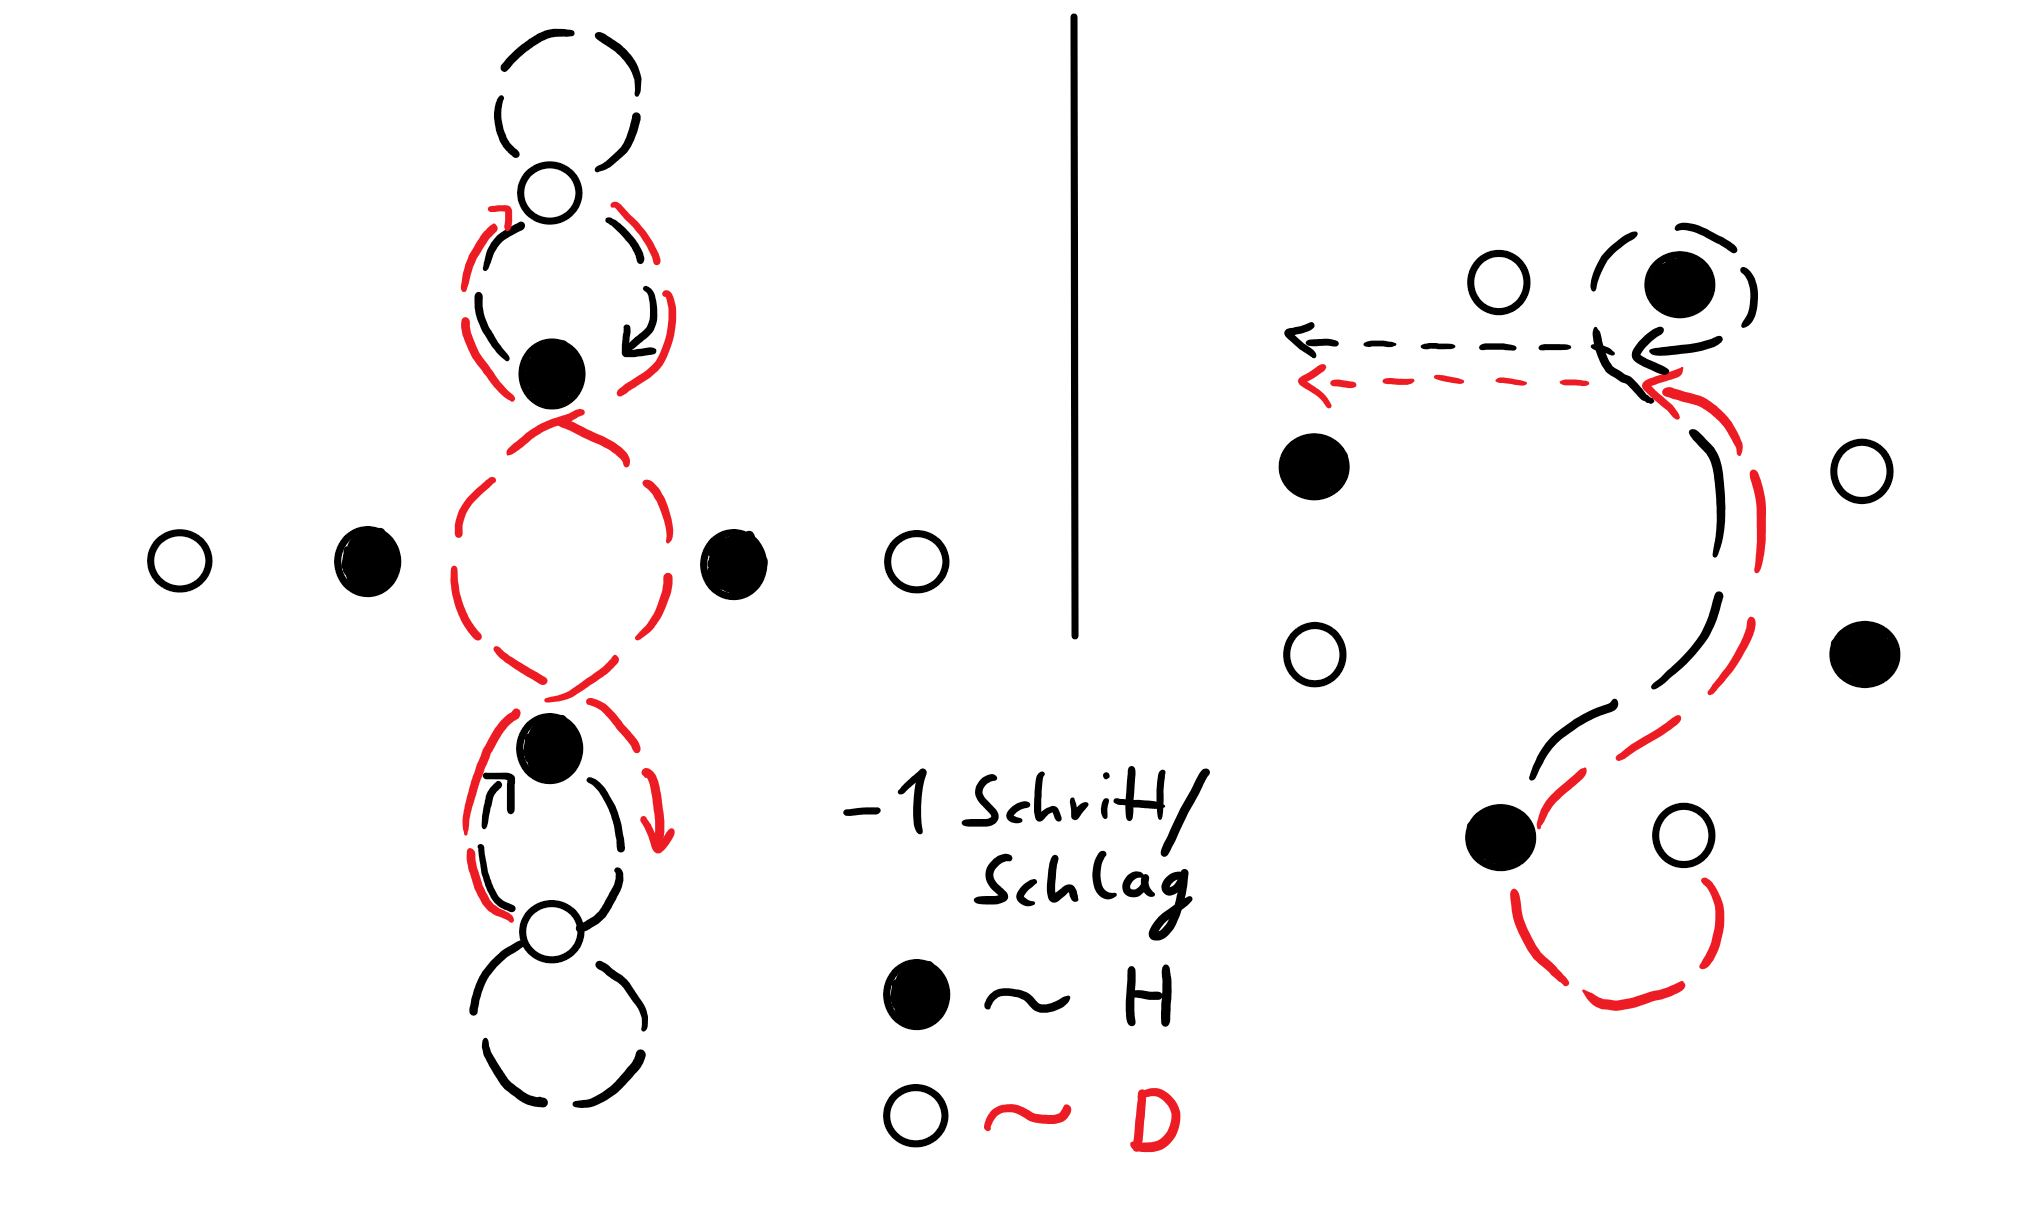
\includegraphics[width=0.65\textwidth]{img/Playing_in_the_Field_2}
\end{center}
\danceinstructionsbegin
13 -- 16 & Herren gelaufene Rechtsdrehung, Damen halber Linkshandstern, damit stehen die Herren rechts neben den Damen\\
\danceinstructionsel
1 -- 4 & Herren führen ihre Dame in die Ecken (in Blick- bzw. Tanzrichtung)\\
5 -- 8 & Die Paare wenden sich zueinander, Doppelhandfassung, der Herr schiebt die Dame in die Seitenmitte\\
1 -- 4 & Head Couples führen in die Setmitte, Side Couples trennen sich rückwärtsgehend\\
5 -- 8 & Head Couples führen jeweils den Kontra aus der Mitte heraus (um 90° drehen), Side Couples drehen sich um 90° und gehen zu ihrem neuen Partner\\
9 -- 12 & Der Herr führt die Dame auf seine rechte Seite
\dancedifficultmarker
\danceinstructionsend


%%%%%%%%%%%%%%%%%%%%%%%%%%%%%%%%%%%%%%%%%%%%%%%%%%%%%%%%%%%%%%%%%%%%%%%%%%%%%%%%
% Puck's Deceit
%%%%%%%%%%%%%%%%%%%%%%%%%%%%%%%%%%%%%%%%%%%%%%%%%%%%%%%%%%%%%%%%%%%%%%%%%%%%%%%%
\newpage

\dancename{Puck's Deceit}
\origininfo{Chris Sackett \& Brooke Friendly (1997)}{Kettle Drum}{Playford}
\iffalse\subsection{Puck's Deceit}\fi % fool texstudio into displaying subsections
\danceinfo{Longway for as many as will}
\danceinstructionsbegin
1--8 & Paar 1 Gipsy, Paar 2 Balancé vor und zurück dann Cast up hinter die Position von Paar 1\\
9--16 & H1 \& Dame 1 passieren sich rechtsschultrig, dann H1 und D2 Gipsy, H2 und D1 Gipsy\\
\danceinstructionsel
1--16 & Hecke rechtsschultrig beginnend, endend in einer Line of four\\
1--8 & Lead up, fall back\\
9--12 & Paar 1 (steht in der Line of four innen) wird von Paar 2 mit einem Gate auf die Tanzlinie geführt\\
13 -- 16 & Halber Gypsy Paar 1
\dancedifficultmarker
\danceinstructionsend


%%%%%%%%%%%%%%%%%%%%%%%%%%%%%%%%%%%%%%%%%%%%%%%%%%%%%%%%%%%%%%%%%%%%%%%%%%%%%%%%
% Queens Jig
%%%%%%%%%%%%%%%%%%%%%%%%%%%%%%%%%%%%%%%%%%%%%%%%%%%%%%%%%%%%%%%%%%%%%%%%%%%%%%%%
\newpage

\dancename{Queens Jig}
\iffalse\subsection{Queens Jig}\fi % fool texstudio into displaying subsections
\danceinfo{Longway for as many as will}
\danceinstructionsbegin
1 -- 8 	& FC Siding\\
9 -- 16 & FC Set \& Turn links\\
1 -- 8 	& SC Siding\\
9 -- 16 & SC Set \& Turn rechts\\
\danceinstructionsel
1 -- 4 	& FC Platzwechsel\\
5 -- 8 	& SC Platzwechsel\\
1 -- 4 	& Balancé zurück\\
5 -- 8 	& Platzwechsel mit Partner\\
\danceinstructionsel
1 -- 12	& volle Mühle (oder vielleicht auch Setkreis)\\
13 -- 16& Turn links\\
\dancemediummarker
\danceinstructionsend


%%%%%%%%%%%%%%%%%%%%%%%%%%%%%%%%%%%%%%%%%%%%%%%%%%%%%%%%%%%%%%%%%%%%%%%%%%%%%%%%
% Red House
%%%%%%%%%%%%%%%%%%%%%%%%%%%%%%%%%%%%%%%%%%%%%%%%%%%%%%%%%%%%%%%%%%%%%%%%%%%%%%%%
\newpage

\dancename{Red House}
\origininfo{Playford (1695)}{Playford}{}
\iffalse\subsection{Red House}\fi % fool texstudio into displaying subsections
\danceinfo{Longway for as many as will}

\danceinstructionsbegin
1 -- 8 	& P1 Meet \& Fallback, P2 Fallback \& Meet\\
1 -- 8  	& P1 Set nach oben, unten, P1 Cast down, P2 lead up\\
1 -- 8 	& P1 Meet \& Fallback, P2 Fallback \& Meet\\
1 -- 8 	& P1 Set nach unten, oben, P1 Cast up, P2 lead down\\
\danceinstructionsel
1 -- 16 	& Herr 1 wendet aus, Dame 1 folgt. Sie gehen einmal um Paar 2 herum. Wenn sie hinter Dame 2 stehen (13) rückt Paar 2 auf und Paar 1 übernimmt den Platz.\\
1 -- 16 	& Dame 2 wendet aus, Herr 2 folgt. Sie gehen einmal um Paar 1 herum. Wenn sie hinter Herr 1 stehen (13) rückt Paar 1 auf und Paar 2 übernimmt den Platz.\\
\danceinstructionsel
\danceinstructionsel
1 -- 16 	& Herr 2 geht mit Paar 1 in eine Hecken-Acht\\
1 -- 12 	& Dame 2 geht in eine Hecken-Acht mit Paar 1 (bisschen zügiger)\\
13 -- 16 	& Paar 1 wendet aus, Paar 2 schließt auf
\dancedifficultmarker
\danceinstructionsend


%%%%%%%%%%%%%%%%%%%%%%%%%%%%%%%%%%%%%%%%%%%%%%%%%%%%%%%%%%%%%%%%%%%%%%%%%%%%%%%%
% Row well, ye mariniers
%%%%%%%%%%%%%%%%%%%%%%%%%%%%%%%%%%%%%%%%%%%%%%%%%%%%%%%%%%%%%%%%%%%%%%%%%%%%%%%%
\newpage

\dancename{Row well, ye mariniers}
\origininfo{Playford (1651)}{Playford}{}
\iffalse\subsection{Row well, ye mariniers}\fi % fool texstudio into displaying subsections
\danceinfo{Longway for as many as will\\1er improper}
\danceinstructionsbegin
1 -- 8 	& Siding links, dann rechts\\
9 -- 12 & Seitgalopp 4 Schritte nach links\\
12--16 	& Seitgalopp 4 Schritte nach rechts\\
1 -- 8 	& Dos-à-dos\\
%\danceinstructionsel
1 -- 8 	& Klatschen:\\
& 1.  Eigene Hände, 2. Beide rechte Hand,\\
& 3. Eigene Hände, 4. Beide linke Hand,\\ & 5. Eigene Hände, 6. rechte Hand eigene Brust, 7. linke Hand eigene Brust, 8. Beide Tänzer beide Hände\\
%\danceinstructionsel
1 -- 4	& Set rechts\\
5 -- 8	& Turn eine Position nach rechts (am Ende auf die andere Seite)
\danceeasymarker
\danceinstructionsend


%%%%%%%%%%%%%%%%%%%%%%%%%%%%%%%%%%%%%%%%%%%%%%%%%%%%%%%%%%%%%%%%%%%%%%%%%%%%%%%%
% Sapphire Sea
%%%%%%%%%%%%%%%%%%%%%%%%%%%%%%%%%%%%%%%%%%%%%%%%%%%%%%%%%%%%%%%%%%%%%%%%%%%%%%%%
% Source for Instructions:
% https://www.youtube.com/watch?v=g-8LyExynvA (Beginning of Video)
% Source for Tune:
% https://www.youtube.com/watch?v=g-8LyExynvA (Beginning of Video)
\newpage

\dancename{Sapphire Sea}
\iffalse\subsection{Sapphire Sea}\fi % fool texstudio into displaying subsections
\origininfo{Christine Robb}{Tom Kruskal's}{von Amelia Mason \& Emily Troll}
\danceinfo{Longway for as many as will}
\danceinstructionsbegin
1 -- 8	& Setkreis links \\
1 -- 8	& First Corner rechte Handtour \\
9 -- 16 & Second Corner linke Handtour \\
\danceinstructionsel
1 -- 8 	& Paar 1 Cast Down, Paar 2 Lead Up \textbf{und} Cast Down an die Enden einer Line of Four mit Paar 1 in der Mitte\\
1 -- 16 	& Dolphin hey von P1, H2, D2, beginnend mit D2, und P1 rechtsschultrig, endet in Line of Four  (H2-H1-D1-D2)\\
\danceinstructionsel
1 -- 8 	& Als Line of Four Lead \& Fall Back \\
9 -- 16 & Paar 2 gatet Paar 1 nach unten ins nächste Set
\dancemediummarker
\danceinstructionsend


%%%%%%%%%%%%%%%%%%%%%%%%%%%%%%%%%%%%%%%%%%%%%%%%%%%%%%%%%%%%%%%%%%%%%%%%%%%%%%%%
% Scales of Justice
%%%%%%%%%%%%%%%%%%%%%%%%%%%%%%%%%%%%%%%%%%%%%%%%%%%%%%%%%%%%%%%%%%%%%%%%%%%%%%%%
% Source for Instructions:
% Tanzbuch Oliver Herde
% Source for Tune:
\newpage

\dancename{Scales of Justice}
\iffalse\subsection{Scales of Justice}\fi % fool texstudio into displaying subsections
\danceinfo{Longway for as many as will}
\origininfo{Chris Sackett \& Brooke Friendly}{Scale of Justice}{Shira Kammen \& Roguery}
\danceinstructionsbegin
1 -- 12 & \nicefrac{3}{4} Kette auf Seitenlinie beginnend\\
\danceinstructionsel
13--16 	& linke Handtour \nicefrac{3}{4} herum\\
1 -- 4 	& Partner lösen Handfassung. Die Inneren tanzen eine rechte \nicefrac{3}{4} Handtour. Die Äußeren gehen \nicefrac{1}{4} auf der Kreisbahn weiter.\\
5 -- 8 	& Paare geben sich die linken Hände zu einer ganzen Handtour\\
9 -- 12	& Die Inneren tanzen wieder \nicefrac{3}{4}, die Äußeren gehen \nicefrac{1}{4} weiter.\\
13--16	& Linke Handtour \nicefrac{3}{4} zurück in die Gasse.\\
\danceinstructionsel
\danceinstructionsel
1 -- 12	& 3x Cecil Sharp Siding links, rechts dann linksschultrig\\
13--16	& Gelaufener Turn rechts\\
1 -- 8 	& Blende\\
9 -- 16	& Ganze Linkhand-Mühle
\dancemediummarker
\danceinstructionsend


%%%%%%%%%%%%%%%%%%%%%%%%%%%%%%%%%%%%%%%%%%%%%%%%%%%%%%%%%%%%%%%%%%%%%%%%%%%%%%%%
% Schiarazula Marazula
%%%%%%%%%%%%%%%%%%%%%%%%%%%%%%%%%%%%%%%%%%%%%%%%%%%%%%%%%%%%%%%%%%%%%%%%%%%%%%%%
\newpage

\dancename{Schiarazula Marazula}
\iffalse\subsection{Schiarazula Marazula}\fi % fool texstudio into displaying subsections
\danceinfo{Kreistanz, Herr/Dame durchgefasst}

\danceinstructionsbegin
1 -- 4	& Doppel nach links, kreuzend(vorne)\\
5 -- 8 	& Doppel nach rechts, kreuzend (vorne)\\
9 -- 16	& Wiederholen\\
\danceinstructionsel
%Nach innen
1 		& Alle setzen einen Fuß nach innen in den Kreis hinein, sodass der 	Fremde Partner angeschaut wird \\
2		& Dem Partner mit beiden Händen zuschnipsen.\\
3 -- 4	& Weiter in den Kreis zum eigenen Partner drehen und schnipsen\\
5 -- 6	& Weiter in den Kreis zum fremden Partner drehen und schnipsen\\
7 -- 8	& Nach außen drehen alle dreimal Klatschen (auf 6, 6\textsuperscript{und}, und 7)\\
\danceinstructionsel
%Nach außen
1 -- 2 	& Nach außen zum fremden Partner drehen und schnipsen\\
3 -- 4 	& Weiter nach außen zum eigenen Partner drehen und schnipsen\\
5 -- 6 	& Weiter nach außen zum eigenen Partner drehen und schnipsen\\
7 -- 8	& Nach innen drehen alle dreimal Klatschen (auf 6, 6\textsuperscript{und}, und 7), 	wieder durchfassen
\danceeasymarker
\danceinstructionsend


%%%%%%%%%%%%%%%%%%%%%%%%%%%%%%%%%%%%%%%%%%%%%%%%%%%%%%%%%%%%%%%%%%%%%%%%%%%%%%%%
% Seepferd und Biber
% Laut dem Arbon Dancing Master: 
% Musik und Choreographie: Ina Lemm
%%%%%%%%%%%%%%%%%%%%%%%%%%%%%%%%%%%%%%%%%%%%%%%%%%%%%%%%%%%%%%%%%%%%%%%%%%%%%%%%
\newpage

\dancename{Seepferd und Biber}
\origininfo{Ina Lemm}{Ina Lemm}{}
\iffalse\subsection{Seepferd und Biber}\fi % fool texstudio into displaying subsections
\danceinfo{Kreistanz, Herren innen, Damen außen\\gerade Anzahl an Paaren}

\textit{Anmerkung: Die Paare sind abwechselnd Seepferde und Biber\\ (Seefperdchen tanzen mit dem vom Herrn aus linken Paar,\\ Biber tanzen mit dem vom Herrn aus rechtem Paar)}
\danceinstructionsbegin

1 -- 16 &	Biber bilden Tore, Seepferde machen eine Figure of Eight hindurch\\
1 -- 16 &	Seepferde bilden Tore, Biber machen eine Figure of Eight hindurch\\
\danceinstructionsel
\textit{Anm.:} & \textit{Drehrichtungen: Biber rechts, Seepferde links}\\

1 -- 4	& Zweimal Klatschen, Zwei Schritte am Partner vorbei, Drehung in Tierrichtung\\
5 -- 8 	& Klatschen, Zwei Schritte am Gegenüber auf Kreisbahn vorbei, Drehung Tierrichtung\\
9 -- 12	& Klatschen, Zwei Schritte am neuen Partner vorbei, in Laufrichtung stehen bleiben\\
13 -- 16& Klatschen, zum Partner umdrehen\\
\danceinstructionsend
\textit{Neuer Partner, Der Tanz beginnt von vorne}
\danceeasymarker


%%%%%%%%%%%%%%%%%%%%%%%%%%%%%%%%%%%%%%%%%%%%%%%%%%%%%%%%%%%%%%%%%%%%%%%%%%%%%%%%
% Siege of Buda
%%%%%%%%%%%%%%%%%%%%%%%%%%%%%%%%%%%%%%%%%%%%%%%%%%%%%%%%%%%%%%%%%%%%%%%%%%%%%%%%
\newpage

\dancename{Siege of Buda}
\origininfo{Playford (1689)}{Playford}{}
\iffalse\subsection{Siege of Buda}\fi % fool texstudio into displaying subsections
\danceinfo{Longway for as many as will}
\danceinstructionsbegin
1 -- 8 	& Paare Dos-á-Dos\\
1 -- 8 	& Dos-á-Dos auf der Linie mit gleichgeschlechtlichem Tänzer\\
\danceinstructionsel
1 -- 4 	& Halber Einhandkreis auf der Linie\\
5 -- 8 	& Fallback im Set durchgefasst\\
9 -- 12	& Meet\\
13 -- 16& Halber Einhandkreis der Paare\\
\danceinstructionsel
1 -- 4	& Halber Setkreis\\
5 -- 8	& P1 Cast down, P2 Lead up
\dancemediummarker
\danceinstructionsend


%%%%%%%%%%%%%%%%%%%%%%%%%%%%%%%%%%%%%%%%%%%%%%%%%%%%%%%%%%%%%%%%%%%%%%%%%%%%%%%%
% Siege of Limerick
%%%%%%%%%%%%%%%%%%%%%%%%%%%%%%%%%%%%%%%%%%%%%%%%%%%%%%%%%%%%%%%%%%%%%%%%%%%%%%%%
\newpage

\dancename{Siege of Limerick}
\origininfo{Playford (1695)}{Playford}{}
\iffalse\subsection{Siege of Limerick}\fi % fool texstudio into displaying subsections
\danceinfo{Longway for as many as will}
\danceinstructionsbegin
1--6 	& H1 cast down, H2 rückt auf\\
7--12 	& H1 geht zwischen Damen durch, um D2, und zurück auf Platz\\
1--6 	& D1 cast down, D2 rückt auf\\
7--12 	& D1 zwischen Herren durch, um H1 rum, und zurück.\\
\danceinstructionsel
1--6 	& P2 cast down, P1 lead up\\
1--6 	& Dos-à-Dos\\
1--12 	& Ganze Kette\\
\danceinstructionsel
1--6 	& P2 Handfassung zu P1 verneigen\\
7--12 	& P1 cast down, P2 lead up
\dancemediummarker
\danceinstructionsend


%%%%%%%%%%%%%%%%%%%%%%%%%%%%%%%%%%%%%%%%%%%%%%%%%%%%%%%%%%%%%%%%%%%%%%%%%%%%%%%%
% 	Siege of St. Malo
%%%%%%%%%%%%%%%%%%%%%%%%%%%%%%%%%%%%%%%%%%%%%%%%%%%%%%%%%%%%%%%%%%%%%%%%%%%%%%%%
\newpage

\dancename{Siege of St. Malo}
\iffalse\subsection{Siege of St. Malo}\fi % fool texstudio into displaying subsections
\danceinfo{Longway for as many as will}

\danceinstructionsbegin
	\danceinstructionsel
	1 -- 8  & First Corner Dos-à-dos\\
	9 -- 16 & Second Corner Dos-à-dos\\
	\danceinstructionsel
	1 -- 8  & $\nicefrac{3}{4}$ Kette\\
	\danceinstructionsel
	1 -- 8  & Set \& Turn rechts
\danceeasymarker
\danceinstructionsend


%%%%%%%%%%%%%%%%%%%%%%%%%%%%%%%%%%%%%%%%%%%%%%%%%%%%%%%%%%%%%%%%%%%%%%%%%%%%%%%%
% Softly Good Tummas
%%%%%%%%%%%%%%%%%%%%%%%%%%%%%%%%%%%%%%%%%%%%%%%%%%%%%%%%%%%%%%%%%%%%%%%%%%%%%%%%
\newpage

\dancename{Softly Good Tummas}
\origininfo{Nathaniel Kynastion (1718)/Andrew Shaw(2002)}{Softly Good Tummas}{Nathaniel Kynastion}
\iffalse\subsection{Softly Good Tummas}\fi % fool texstudio into displaying subsections
\danceinfo{Longway for as many as will}
\danceinstructionsbegin
1 -- 8 	& Halber Single file circle links (UZS)\\
9 -- 12 & Meet in der Setmitte\\
13--16 	& Turn links zurück -- auf 16 klatschen\\
1 -- 16 & Wiederholung rechts\\
\danceinstructionsel
1 -- 4 	& Paar 1 Cast down, Paar 2 lead up\\
5 -- 8 	& Setting steps links, rechts\\
9 -- 16 & Halbe Kette\\
\danceinstructionsel
1 -- 4 	& Setting steps zurück (Anlauf nehmen)\\
5 -- 8 	& Platzwechsel mit dem Partner\\
9 -- 16 & Paar 1 rondiert nach unten, Past 2 cast up
\dancemediummarker
\danceinstructionsend


%%%%%%%%%%%%%%%%%%%%%%%%%%%%%%%%%%%%%%%%%%%%%%%%%%%%%%%%%%%%%%%%%%%%%%%%%%%%%%%%
% St. Martins Lane
%%%%%%%%%%%%%%%%%%%%%%%%%%%%%%%%%%%%%%%%%%%%%%%%%%%%%%%%%%%%%%%%%%%%%%%%%%%%%%%%
\newpage


\dancename{St. Martins Lane}
\iffalse\subsection{St. Martins Lane}\fi % fool texstudio into displaying subsections
\origininfo{Playford}{La Furstemberg}{Anonymous} % Or maybe Purcell: https://www.jstor.org/stable/737425
\danceinfo{Triple Minor Longway, \nicefrac{4}{4} Takt}
\danceinstructionsbegin
\danceinstructionsel
1 -- 4 & H1 wendet hinter H2 aus und geht zwischen H2 und H3 hindurch zu D3\\
5 -- 12 & H1 \& D3 Ronde\\
13 -- 16 & H1 zwischen H2 \& H3 zurück auf seinen Platz\\
\danceinstructionsel
1 -- 4 & D1 wendet hinter D2 aus und geht zwischen D2 und D3 hindurch zu H3\\
5 -- 12 & H1 \& D3 Ronde\\
13 -- 16 & H1 zwischen H2 \& H3 zurück auf seinen Platz\\
\danceinstructionsel
\danceinstructionsel
\danceinstructionsel

1 -- 4 & P1 Lead Down zwischen P3\\
5 -- 16 & P3 Cast Up, P1 Cross Down, und dann Rest einer doppelten Figure eight gehen, sodass P1 proper auf Position 2 endet.\\
\danceinstructionsel
1 -- 4 & P1 Lead Up zwischen P2 (auf Position 1)\\
5 -- 16 & P2 Cast Down, P1 Cross Up, ... doppelte Figure eight, sodass P1 proper auf Position 2 endet.\\
\danceinstructionsel
1 -- 8 & Triple Minor Longway: P1 Ronde\\
& Longway for six: P1 mit Ronde auf Position 3 kreiseln, P3 Cast Up\\
\dancedifficultmarker
\danceinstructionsend



%%%%%%%%%%%%%%%%%%%%%%%%%%%%%%%%%%%%%%%%%%%%%%%%%%%%%%%%%%%%%%%%%%%%%%%%%%%%%%%%
% Tango in Toronto
%%%%%%%%%%%%%%%%%%%%%%%%%%%%%%%%%%%%%%%%%%%%%%%%%%%%%%%%%%%%%%%%%%%%%%%%%%%%%%%%
\newpage


\dancename{Tango in Toronto}
\iffalse\subsection{Tango in Toronto}\fi % fool texstudio into displaying subsections
\origininfo{Colin Hume}{Tango in Toronto}{von Colin Hume} 
\danceinfo{Longway, Duple Minor}
\danceinstructionsbegin
1 -- 8 & FC: H1 Double vor, D2 Double rückwärts und zurück.\\
9 -- 16 & FC Gypsy linksschultrig, am Ende Turn rechts.\\
1 -- 8 & Rechthandstern ganz herum. Am Ende Partner rechte Hand geben.\\
9 -- 16 & Partner halbe rechte Handtour, dann Turn links.\\
\danceinstructionsel
1 -- 8 & SC: D1 Double vor, H2 Double rückwarts und zurück.\\
9 -- 16 & FC Gypsy rechtsschultrig, am Ende Turn links.\\
1 -- 8 & Linkshandstern ganz herum. Am Ende Partner links Hand geben.\\
9 -- 16 & Partner halbe linke Handtour, dann Turn rechts.\\
\danceinstructionsel
\danceinstructionsel
1 -- 24 & Halbe Hey + Gypsy + Halbe Hey:\\
 & FC starten eine halbe Hey rechtsschultrig. SC steigen ein, sobald sich FC passiert haben und starten mit eigenem Partner linkschultrig.\\
 & Nach einer halben Hey begegnen sich die FC und tanzen einen halben Gypsy rechtsschultrig (ergo eine halbe Drehung), dann eine weitere halbe Hey.\\
 & Man endet, sodass Fortschritt erzielt wurde. (nachdem sich die FC passiert haben)\\
1 -- 8 & Ganzer Setkreis ohne Anfassen (original: Single file circle)\\
\dancedifficultmarker
\danceinstructionsend
\vspace{-0.1cm}
\textit{Wie Colin Hume auch schon anmerkt sollte man darauf achten die Hey nicht diagonal sondern rechtwinklig zum Longway zu tanzen. Es kann helfen, wenn die SC einen Schritt nach links hinten machen, um von dort in die Hey zu starten.}


%%%%%%%%%%%%%%%%%%%%%%%%%%%%%%%%%%%%%%%%%%%%%%%%%%%%%%%%%%%%%%%%%%%%%%%%%%%%%%%%
% Tanz der Karibik
%%%%%%%%%%%%%%%%%%%%%%%%%%%%%%%%%%%%%%%%%%%%%%%%%%%%%%%%%%%%%%%%%%%%%%%%%%%%%%%%
%\iffalse
\newpage

\dancename{Tanz der Karibik}
\origininfo{Oliver Herde}{Davy Jones}{von Hans Zimmer}
\iffalse\subsection{Tanz der Karibik}\fi % fool texstudio into displaying subsections
\danceinfo{Gasse ohne Fortschritt, ¾ Takt}
\danceinstructionsbegin
\multicolumn{2}{c}{\textbf{Verträumter Auftakt}}\\
\danceinstructionsel
& \textit{In die Setmitte schauend}\\
1 -- 6 	& Balancé rechts \& links\\
7 -- 12	& Turn rechts\\
1 -- 3 	& FC passieren sich linksschultrig, SC Balancé rechts\\
4 -- 6 	& FC in der gegenüberliegenden Corner noch einmal dem eigenen Partner zuwenden (über die linke Schulter) und dann nach rechts wenden\\
& SC Balancé rechts\\
7 -- 12 & FC gehen um die SC herum auf ihren Platz zurück, SC Turn rechts (sie können dabei den vorbeigehenden gleichgeschlechtlichen Kontra anschauen.)\\
\danceinstructionsel
1 -- 6 	& Balancé links \& rechts\\
7 -- 12	& Turn links\\
1 -- 3 	& SC passieren sich rechtsschultrig, FC Balancé links\\
4 -- 6 	& SC in der gegenüberliegenden Corner noch einmal dem eigenen Partner zuwenden (über die rechte Schulter) und dann nach links wenden\\
& FC Balancé rechts\\
7 -- 12 & SC gehen um die FC herum auf ihren Platz zurück, FC Turn rechts (sie können dabei den vorbeigehenden gleichgeschlechtlichen Kontra anschauen.)\\
\danceinstructionsel
1 -- 12 & Ganze Kette mit Partner beginnend\\
13--24 	& Ganze Kette zurück\\
1 -- 6 	& Paar 1 geht durch Paar 2 nach unten, Paar 2 Balancé oben, unten\\
7 -- 12 & Paar 1 geht wieder zurück, Paar 2 Drehung oben (walzt praktisch P1 zurürck)\\
1 -- 6 	& Paar 1 Cast down, Paar 2 Balancé down und lead up\\
7 -- 12 & Ronde mit Partner\\
\danceinstructionsel
\multicolumn{2}{c}{\textit{Kurze Pause, Tempowechsel}}\\
\multicolumn{2}{c}{\textbf{Machtvoller Hauptteil}}\\
\danceinstructionsel
1 -- 6 & Balancé nach unten, nach oben (jeder sein eigenes)\\
1 -- 12 & Paar 2 Lead Down und Cast Up, Paar 1 Set \& Turn unten\\
1 -- 12 & Paar 1 Lead Up und Cast Down, Paar 2 Set \& Turn oben\\
1 -- 12 & Paar 2 Cross Down und Cast Up, Paar 1 Set \& Turn unten\\
1 -- 12 & Ronde mit Partner\\
\danceinstructionsel
%\danceinstructionsel % um einen sauberen Seitenumbruch zu kriegen
1 -- 12 & Dosado auf der Linie\\
1 -- 12 & Ronde auf der Linie\\
1 -- 12 & Dosado mit dem Partner\\
1 -- 6 & halbe Ronde mit dem Partner\\
7 -- 12 & Paar 2 Cast Down, Paar 1 mit weiterer halben Ronde nach oben aufrücken\\
\danceinstructionsel
1 -- 6 & Rechte Hände gefasst Balancé vor \& zurück\\
7 -- 12 & Platzwechsel (unter Arm durchdrehen)\\
1 -- 12 & Wiederholung links (linke Hände, Balancé vor \& zurück, Platzwechsel)\\
1 -- 12 & Hohe rechte Handtour\\
1 -- 12 & Hohe linke Handtour\\
\danceinstructionsel
1 -- 3 & Referenz zum Partner\\
4 -- 6 & Referenz noch tiefer machen\\
7 -- 9 & Wieder halb aufrichten\\
10--12 & Ganz aufrichten\\
1 -- 12 & Wiederholen in Richtung Setmitte\\

\danceinstructionsel
\multicolumn{2}{c}{\textit{Kurze Pause, Tempowechsel}}\\
\multicolumn{2}{c}{\textbf{Verträumter Abschluss}}\\
\danceinstructionsel

& \textit{In die Setmitte schauend}\\
1 -- 12 & Set \& Turn Rechts\\
1 -- 12 & Rechthandstern ganz herum\\
1 -- 9 & Linkhandstern zurück\\
10--12 & Stern fertig laufen, Herren nehmen ihre eigene Dame an die rechte Hand (also Herr rechte, Dame linke Hand, gefasst)\\
1 -- 12 & In dieser Haltung die Kreisbewegung mit einer ganzen Ronde gegen den UZS fortführen\\
\danceinstructionsel
\multicolumn{2}{c}{\textit{Abschließende Referenz}}\\
\dancedifficultmarker
\danceinstructionsend
%\fi

%%%%%%%%%%%%%%%%%%%%%%%%%%%%%%%%%%%%%%%%%%%%%%%%%%%%%%%%%%%%%%%%%%%%%%%%%%%%%%%%
% The Chocolate Equation
%%%%%%%%%%%%%%%%%%%%%%%%%%%%%%%%%%%%%%%%%%%%%%%%%%%%%%%%%%%%%%%%%%%%%%%%%%%%%%%%
% \newpage

% \dancename{The Chocolate Equation}
%\origininfo{Brooke Friendly \& Chirs Sackett}{72\%}{von Shira Kammen}
\iffalse \subsection{[The Chocolate Equation]}\fi % fool texstudio into displaying subsections
% \danceinfo{}
% \danceinstructionsbegin
% \danceinstructionsend
% \dancedifficultmarker


%%%%%%%%%%%%%%%%%%%%%%%%%%%%%%%%%%%%%%%%%%%%%%%%%%%%%%%%%%%%%%%%%%%%%%%%%%%%%%%%
% The Crossroads
% Video: https://www.youtube.com/watch?v=t_mkdMxuZ6Y
%%%%%%%%%%%%%%%%%%%%%%%%%%%%%%%%%%%%%%%%%%%%%%%%%%%%%%%%%%%%%%%%%%%%%%%%%%%%%%%%
\newpage

\iffalse\subsection{The Crossroads}\fi % fool texstudio into displaying subsections
\dancename{The Crossroads}
\danceinfo{Tanz für 4 Paare,\\P1\&P2 improper}
\origininfo{Sascha Glimmann}{Soldier Boy}{von Custer LaRue}
\danceinstructionsbegin
1 -- 4 &  Set links zum Partner\\
5 -- 8 &  Halber Ronde\\
9 -- 16 & Paare Dos-á-Dos\\
1 -- 8 &  Setkreis je 2 Paare\\
9 -- 16 & Außenpaare gaten Innenpaare nach außen \nicefrac{3}{4} herum, sodass der Longway um 90° gedreht endet.\\
\dancemediummarker
\danceinstructionsend


%%%%%%%%%%%%%%%%%%%%%%%%%%%%%%%%%%%%%%%%%%%%%%%%%%%%%%%%%%%%%%%%%%%%%%%%%%%%%%%%
% The Gun
%%%%%%%%%%%%%%%%%%%%%%%%%%%%%%%%%%%%%%%%%%%%%%%%%%%%%%%%%%%%%%%%%%%%%%%%%%%%%%%%
\newpage

\iffalse\subsection{[The Gun]}\fi % fool texstudio into displaying subsections
\dancename{The Gun}
\danceinfo{Duple Minor Longway}
\origininfo{Playford 1651}{Playford}{}
\danceinstructionsbegin
\textbf{Teil} & \textbf{I}~~~ (Leading)\\
1 -- 8 & Lead Up and Back\\
9 -- 16 & Set \& Turn Links\\
1 -- 16 & Wiederholen (Rechts)\\
\danceinstructionsel
1 -- 8 & Herren- \& Damenlinien: Fall back \& Meet\\
9 -- 12 & First Corner Platzwechsel\\
13--16 & Second Corner Platzwechsel\\
1 -- 16 & Wiederholen (Doppelter Fortschritt, 1er bleiben in ihren Rollen, die zweiten FC sind in der üblichen SC Position)\\
& \textit{Bäumchen müssen je nach Stelle einen Platzwechsel machen.}\\
\danceinstructionsel
\textbf{Teil} & \textbf{II}~~~ (Siding)\\
1 -- 8 & Siding Links\\
9 -- 16 & Set \& Turn Links\\
1 -- 16 & Wiederholen (Rechts)\\
\danceinstructionsel
1 -- 8 & Ganzer Setkreis \\
9 -- 12 & Seitgalopp 1er innen nach unten, 2er außen hoch\\
13 -- 16 & Turn (1er: unten, 2er: oben)\\
1 -- 16 & Wiederholen (Doppelter Fortschritt)\\
\danceinstructionsel
\textbf{Teil} & \textbf{III}~~~ (Armtour)\\
1 -- 8 & Armtour Links (mit rechten Armen)\\
9 -- 16 & Set \& Turn Links\\
1 -- 16 & Wiederholen (Rechts)\\
\danceinstructionsel
1 -- 4 & Herren Platzwechsel, dabei Schnipsen (1er innen)\\
5 -- 8 & Damen Platzwechsel, dabei Schnipsen (1er innen)\\
9 -- 16 & Mühle rechts mit den bisherigen Setpartnern\\
1 -- 16 & Wiederholen (Doppelter Fortschritt)\\
\dancedifficultmarker
\danceinstructionsend



%%%%%%%%%%%%%%%%%%%%%%%%%%%%%%%%%%%%%%%%%%%%%%%%%%%%%%%%%%%%%%%%%%%%%%%%%%%%%%%%
% The Homecoming
%%%%%%%%%%%%%%%%%%%%%%%%%%%%%%%%%%%%%%%%%%%%%%%%%%%%%%%%%%%%%%%%%%%%%%%%%%%%%%%%
\newpage

\iffalse\subsection{The Homecoming}\fi % fool texstudio into displaying subsections
\dancename{The Homecoming}
\origininfo{Gary Roodman(1997)}{The Homecoming}{Jonathan Jensen (1997)}
\danceinfo{Duple Minor Longway,\\1er improper}
\danceinstructionsbegin
1 -- 12 & H1 wendet aus, geht unter P2 entlang, und hinter H2 auf den vorigen Platz von D1, D1 folgt H1, geht aber nicht hinter H2 zurück, sondern "kürzt" zwischen P2 hindurch ab, auf den vorigen Platz von H1\\
1 -- 12 & P2 ebenso: H2 wendet aus, D2 folgt, auf jeweils andere Plätze. Sie werden aber ab ca. der Hälfte vom Contra Partner in eine Line-of-Four gegatet.\\
\danceinstructionsel
1 -- 12 & Line-of-Four: 6 Schritte hoch, dabei nach 3 Schritten umdrehen, aber Laufrichtung beibehalten. 6 Schritte ebenso wieder zurück. Zum Contra drehen.\\
1 -- 12 & \nicefrac{1}{2} Hecke, dann Kontrapaare \nicefrac{3}{4} Ronde und nach außen schauen (z.B. Hecke 8, Ronde 4 Schläge).\\
1 -- 3 & Contrapaare führen nach außen\\
4 -- 6 & Contrapaare drehen sich wieder nach innen und führen zurück\\
7 -- 9 & Platzwechsel Damen\\
10--12 & Platzwechsel Herren\\
\danceinstructionsel
1 -- 6 & Halber Setkreis \\
7 -- 12 & Paare Ganze Ronde \\
\danceinstructionsel
\danceinstructionsend
\dancedifficultmarker


%%%%%%%%%%%%%%%%%%%%%%%%%%%%%%%%%%%%%%%%%%%%%%%%%%%%%%%%%%%%%%%%%%%%%%%%%%%%%%%%
% The Introduction
% Music Source: https://tunearch.org/wiki/Annotation:Carolan%27s_Cottage
%%%%%%%%%%%%%%%%%%%%%%%%%%%%%%%%%%%%%%%%%%%%%%%%%%%%%%%%%%%%%%%%%%%%%%%%%%%%%%%%
\newpage

\dancename{The Introduction}
\origininfo{Fried de Metz Herman}{Carolans Cottage}{Turlough O'Carolan}
\iffalse\subsection{The Introduction}\fi % fool texstudio into displaying subsections
\danceinfo{Longway for four couples\\¾ Takt}
\danceinstructionsbegin
1 -- 12	& Pos 1 Auswenden auf Pos 3, Pos 2+3 aufrücken\\
1 -- 6 	& Pos 3+4 Rechthand-Stern halb herum\\
7 -- 12	& Pos 2+3 Linkhand-Stern halb herum\\
1 -- 24 & Wiederholung\\
\danceinstructionsel
1 -- 24 & 4x Diagonaler Platzwechsel: R/L/R/L\\
& \textit{(Wenn kein Wechselpartner da ist, stehen bleiben)}\\
\danceinstructionsel
1 -- 12	& Pos 3 lead up, cast down auf Pos 4, 4er rücken auf\\
13--24 	& Alle 1 bzw. 1\nicefrac{1}{2} Ronden bis man wieder proper steht
\dancedifficultmarker
\danceinstructionsend


%%%%%%%%%%%%%%%%%%%%%%%%%%%%%%%%%%%%%%%%%%%%%%%%%%%%%%%%%%%%%%%%%%%%%%%%%%%%%%%%
% Tourdion
%%%%%%%%%%%%%%%%%%%%%%%%%%%%%%%%%%%%%%%%%%%%%%%%%%%%%%%%%%%%%%%%%%%%%%%%%%%%%%%%
\newpage

\dancename{Tourdion}
\origininfo{???}{???}{}
\iffalse\subsection{Tourdion}\fi % fool texstudio into displaying subsections
\danceinfo{Kreistanz, Herr/Dame, durchgefasst}
\danceinstructionsbegin
1--4 	& Nach links, rechts vor und zurück wiegen\\
5--16 	& 3x Wiederholen \\
\danceinstructionsel
1--2 	& Die Herren geben/heben/werfen die rechts stehende Dame einen Platz nach links, danach \\
3--4 	& Vor und zurück wiegen\\
5--16 	& 3x Wiederholen \\
\danceinstructionsel
1--16 	& Grundschritt: Links, rechts, vor, zurück (x4)\\
%\danceinstructionsel
1--4 	& Die Damen geben/heben/werfen den links stehenden Herren einen Platz nach rechts, danach Vor und zurück wiegen\\
5--16 	& 3x Wiederholen
\danceeasymarker
\danceinstructionsend


%%%%%%%%%%%%%%%%%%%%%%%%%%%%%%%%%%%%%%%%%%%%%%%%%%%%%%%%%%%%%%%%%%%%%%%%%%%%%%%%
% Traubentritt
%%%%%%%%%%%%%%%%%%%%%%%%%%%%%%%%%%%%%%%%%%%%%%%%%%%%%%%%%%%%%%%%%%%%%%%%%%%%%%%%
\newpage

\dancename{Traubentritt}
\origininfo{???}{???}{}
\iffalse\subsection{Traubentritt}\fi % fool texstudio into displaying subsections
\danceinfo{Longway for as many as will}
\danceinstructionsbegin
1--8 	& vier Simpel abwechselnd links und rechts, auf 8 umdrehen\\
9--16 	& vier Simpel zurück – zueinander wenden\\
\danceinstructionsel
1--4	 	& Referenz Herren\\
5--8 	& Referenz Damen\\
9--12 	& Referenz Links\\
13--16 	& Referenz Rechts\\
\danceinstructionsel
1--6 	& Die Dame dreht dreimal unter der rechten Hand des Herren\\
7--8	& Referenz beider\\
9--12	& Der hinterste Herr läuft durch die Gasse an die Spitze, alle anderen Herren rücken mit zwei Anstellschritten auf
\danceeasymarker
\danceinstructionsend


%%%%%%%%%%%%%%%%%%%%%%%%%%%%%%%%%%%%%%%%%%%%%%%%%%%%%%%%%%%%%%%%%%%%%%%%%%%%%%%%
% Ungaresca
%%%%%%%%%%%%%%%%%%%%%%%%%%%%%%%%%%%%%%%%%%%%%%%%%%%%%%%%%%%%%%%%%%%%%%%%%%%%%%%%
\newpage

\dancename{Ungaresca}
\iffalse\subsection{Ungaresca}\fi % fool texstudio into displaying subsections
\danceinfo{Kreistanz, Herren innen, Damen außen, GUZS}
\danceinstructionsbegin
1 -- 8 	& Doppel vor und zurück\\
9 -- 16 & Wiederholen am Ende zueinander drehen\\
\danceinstructionsel
1 -- 4 	& 2 Branle-Schritte nach links\\
5 -- 8 	& 2 Branle-Schritte nach rechts\\
9 -- 12 & Platzwechsel mit dem Partner\\
\danceinstructionsel
1 -- 4 	& 2 Branle-Schritte nach links (gegenüber merken)\\
5 -- 8 	& 2 Branle-Schritte nach rechts\\
9 -- 12 & Platzwechsel linke Hand mit gemerkter Person
\danceeasymarker
\danceinstructionsend


%%%%%%%%%%%%%%%%%%%%%%%%%%%%%%%%%%%%%%%%%%%%%%%%%%%%%%%%%%%%%%%%%%%%%%%%%%%%%%%%
% Upon a Summers Day
%%%%%%%%%%%%%%%%%%%%%%%%%%%%%%%%%%%%%%%%%%%%%%%%%%%%%%%%%%%%%%%%%%%%%%%%%%%%%%%%
\newpage

\dancename{Upon a Summers Day}
\origininfo{Playford (1651)}{Playford}{}
\iffalse\subsection{Upon a Summers Day}\fi % fool texstudio into displaying subsections
\danceinfo{Longway for six}

\danceinstructionsbegin
\textbf{Strophe} & \textbf{~I}\\
1--8 	& Lead Up and Down\\
9--16 	& Set \& Turn links\\
1--16 	& Wiederholung (rechts)\\
\danceinstructionsel
\textbf{Refrain}& \\
1--8 	& Meet \& Fallback\\
9--16 	& Paar 1 nach hinten schlängeln, aufrücken\\
1--16 	& Wiederholen (Paar 2)\\
1--16 	& Wiederholen (Paar 3)\\
\danceinstructionsel
\textbf{Strophe} & \textbf{~II}\\
1--8 	& Siding links\\
9--16 	& Set \& Turn links\\
1--16 	& Wiederholen (rechts)\\
\danceinstructionsel
1-48 	& \textbf{Refrain}\\
\danceinstructionsel
\textbf{Strophe} & \textbf{~III}\\
1--8 	& Handtour links\\
9--16 	& Set \& Turn links\\
1--16 	& Wiederholung (rechts)\\
\danceinstructionsel
1--48 	& \textbf{Refrain}\\
\danceinstructionsend
\textit{(Keine Wiederholung)}
\dancemediummarker


%%%%%%%%%%%%%%%%%%%%%%%%%%%%%%%%%%%%%%%%%%%%%%%%%%%%%%%%%%%%%%%%%%%%%%%%%%%%%%%%
% Ursa Minor
%%%%%%%%%%%%%%%%%%%%%%%%%%%%%%%%%%%%%%%%%%%%%%%%%%%%%%%%%%%%%%%%%%%%%%%%%%%%%%%%
\newpage

\dancename{Ursa Minor}
% Dimensionen ausprobiert, dass sie nicht mit den 41er Ornamenten in den Ecken kollidieren.
%\begin{textblock}{4}(1.3,12.6)
%	\begin{flushleft}
	%		{\scriptsize Choreographie:\\[-0.2cm] Brooke Friendly \& Chris Sackett}
	%	\end{flushleft}
%\end{textblock}
%
%\begin{textblock}{4}(10.7,12.6)
%	\begin{flushright}
	%		{\scriptsize Musik:\\[-0.2cm] Roguery(2010)}
	%	\end{flushright}
%\end{textblock}
\origininfo{Chris Sackett \& Brooke Friendly}{Ursa Minor}{von Roguery(2010)}

\iffalse \subsection{Ursa Minor}\fi % fool texstudio into displaying subsections
\danceinfo{Longway for as many as will}
\danceinstructionsbegin
1 -- 8 & Siding links \\
9 -- 16 & P1 Cross down \& Cast up ~~|~~ P2 Cast up \& Cross down\\
1 -- 8 & Mirror Siding (P1 in der Mitte nach unten P2 außen nach oben)\\
1 -- 8 & Handtour der Herren und Damen (H links, D rechts)\\
1 -- 4 & Lead Down innen Paar 1, Lead up außen Paar 2 (Travel)\\
5 -- 8 & Set \& Turn rechts\\
9 -- 12 & Lead back up Paar 1, Lead back down Paar 2\\
13 -- 16 & Paar 1 Cast Down, Paar 2 Lead up\\
1 -- 8 & P1 Cross Up \& Cast Down ~~|~~ P2 Cast Down \& Cross Up\\
9 -- 16 & Ronde mit dem Partner
\dancedifficultmarker
\danceinstructionsend


%%%%%%%%%%%%%%%%%%%%%%%%%%%%%%%%%%%%%%%%%%%%%%%%%%%%%%%%%%%%%%%%%%%%%%%%%%%%%%%%
% Vivaldi in Paradise
%%%%%%%%%%%%%%%%%%%%%%%%%%%%%%%%%%%%%%%%%%%%%%%%%%%%%%%%%%%%%%%%%%%%%%%%%%%%%%%%
\newpage

\dancename{Vivaldi in Paradise}
\origininfo{Gary Roodman (2005)}{Vivaldi in Paradise}{Van Kaynor (?)}
\iffalse\subsection{Vivaldi in Paradise}\fi % fool texstudio into displaying subsections
\danceinfo{}
\danceinstructionsbegin
1 -- 8	& P1 lead down durch P2 und cast up zurück zum Platz\\
9 -- 16	& P1 lead up zum drüberstehenden P2 aus dem nächsten Set und lead down zurück zum Platz (Der Übergang all dieser Figuren ist fließend)\\
1 -- 16	& P2 dito, nur gespiegelt (also lead up, cast down, lead down, lead up)\\
1 -- 4	& Rechtsschultrig den Nachbarn passieren\\
5 -- 8	& Mit der entgegenkommenden Person aus dem nächsten Set Gipsy linksherum (GUZS), man schaut danach wieder zurück ins eigene Set\\
9 -- 16	& Mit dem Nachbarn Gipys rechtsherum (UZS)\\
1 -- 4 	& Herren Platzwechsel\\
5 -- 8 	& Damen Platzwechsel\\
9 -- 12	& Rechtsschultrig den Nachbarn passieren\\
13--16 	& \nicefrac{1}{2} Ronde mit dem Partner
\dancedifficultmarker
\danceinstructionsend


%%%%%%%%%%%%%%%%%%%%%%%%%%%%%%%%%%%%%%%%%%%%%%%%%%%%%%%%%%%%%%%%%%%%%%%%%%%%%%%%
% Walenki
%%%%%%%%%%%%%%%%%%%%%%%%%%%%%%%%%%%%%%%%%%%%%%%%%%%%%%%%%%%%%%%%%%%%%%%%%%%%%%%%
\newpage

\dancename{Walenki}
\origininfo{???}{???}{}
\iffalse \subsection{Walenki}\fi % fool texstudio into displaying subsections
\danceinfo{Doppelter Kreis, Damen innen, \\Herren versetzt außen,\\ beide Kreise durchgefasst}
\danceinstructionsbegin
1 -- 8 & Die Herren gehen 8 Schritte links herum, die Damen 8 Schritte rechts\\
9 -- 16 & Die Herren 8 Schritte rechts zurück, die Damen 8 Schritte links zurück\\
\danceinstructionsel
1 -- 8 & Alle gehen gemeinsam in die Mitte und wieder zurück\\
1 -- 4 & Wieder alle in die Mitte, die Herren heben die Hände\\
5 -- 8 & Alle wieder zurück, die Herren fangen die Damen mit den Händen ein\\
1 -- 16 & Alle 8 Schritte rechts, dann 8 Schritte links\\
1 -- 8 & Alle gehen gemeinsam in die Mitte und wieder zurück\\
1 -- 8 & Alle gehen gemeinsam in die Mitte, die Herren heben die Hände wieder über die Damen zurück\\
1 -- 16 & Die Herren gehen 8 Schritte links, die Damen 8 Schritte rechts und wieder zurück\\
1 -- 8 & Tore: Die Damen heben die Hände und gehen nach außen, die Herren darunter hindurch, dann heben die Herren ihre Hände und gehen nach außen, die Damen gehen durch die Tore.\\
9 -- 16 & Wiederholung
\danceeasymarker
\danceinstructionsend


%%%%%%%%%%%%%%%%%%%%%%%%%%%%%%%%%%%%%%%%%%%%%%%%%%%%%%%%%%%%%%%%%%%%%%%%%%%%%%%%
% Well's Humour
%%%%%%%%%%%%%%%%%%%%%%%%%%%%%%%%%%%%%%%%%%%%%%%%%%%%%%%%%%%%%%%%%%%%%%%%%%%%%%%%
\newpage

\dancename{Well's Humour}
\origininfo{???}{???}{}
\iffalse\subsection{Well's Humour}\fi % fool texstudio into displaying subsections
\danceinfo{Longway for as many as will\\¾ Takt\\(original für 3 Paare)}
\danceinstructionsbegin
1 -- 3 	& Paar 1 passiert sich rechtschultrig\\
4 -- 9 	& Paar 1 geht außen um Paar 2 nach unten, Paar 2 geht auf 7 -- 9 nach oben\\
10--12& Paar 1 geht zwischen das von unten hochkommende Paar 2\\
1 -- 6 	& Paar 1 kreuzt zwischen Paar 2 hindurch und geht um es herum, Paar 2 dreht sich um\\
7 -- 12 & Paar 1 geht außerhalb von Paar 2 auf ihre Startplätze zurück. Paar 2 rückt wieder nach unten\\
& (Tanzbuch:) 9 -- 12 : Paar 1 Turn außen\\
\danceinstructionsel
\danceinstructionsel
1 -- 3 	& Platztausch FC\\
4 -- 6 	& Platztausch SC\\
7 -- 12 & halber Setkreis\\
1 -- 12 & \nicefrac{3}{4} Kette
\dancedifficultmarker
\danceinstructionsend


%%%%%%%%%%%%%%%%%%%%%%%%%%%%%%%%%%%%%%%%%%%%%%%%%%%%%%%%%%%%%%%%%%%%%%%%%%%%%%%%
% Winter Solstice
% Video: https://www.youtube.com/watch?v=dEKuxMqWSGE
% Video + Explanation: https://www.youtube.com/watch?v=a_sbaB6YZQE
%%%%%%%%%%%%%%%%%%%%%%%%%%%%%%%%%%%%%%%%%%%%%%%%%%%%%%%%%%%%%%%%%%%%%%%%%%%%%%%%
\newpage

\dancename{Winter Solstice}
\origininfo{Wendy Crouch (1998)}{Early One Morning}{Traditional}
\iffalse\subsection{Winter Solstice}\fi % fool texstudio into displaying subsections
\danceinfo{Grand Square mit Center Couple, das zu Paar 1 gewendet steht.}

\danceinstructionsbegin
1 -- 16  & Head Couple + Center Couple Spiegelhecke (ähnlich zum Refrain des Grimstock), Side Couple: Siding + Set \& Turn.\\
17--32 & Center Couple teilt sich und gehen jeweils mit den Side Couples in eine Acht. Head Couples: Siding + Set \& Turn.\\
\danceinstructionsel
~  & \textbf{Grand Square Figur}: \\
1 -- 8 & Head Couples Meet in der Mitte und umfassen, dann Fall back auf die Plätze der Side Couples. \\
~ & Side Couples Fall back und Meet mit dem Contra zur Position der Head Couples. \\
~ & Center Couple Fall back auf Side Couple Position, dann weiter Fall Back auf die Ecken neben Position 3.\\
9 -- 16 & Head \& Side Couples wiederholen die Bewegung der jeweils anderen, um wieder auf den eigenen Plätzen zu enden. Center Couple Meet auf Position 3 und in die Mitte führen.\\
\danceinstructionsel
~ & \textbf{„Promenadenfortschritt“:}\\
~ & \textit{Alle in doppelter Handhaltung (nebeneinander, überkreuzt)}\\
1 -- 4 & Center Couple mit Paar 1 „linksschultrig“ den Platz tauschen.\\
5 -- 8 & Paar 1 mit Paar 2 „linksschultrig“ den Platz tauschen.\\
9 -- 12 & Ebenso Paar 2 mit Paar 3\\
13 -- 16 & Ebenso Paar 3 mit Paar 4. Paar 4 ist neues Center Couple.\\

~ & \textit{Diese Platzwechsel gehen sehr schön ineinander über, es wird immer ein durchgehender Bogen nach links gelaufen.}
\origininfo{Wendy Crouch}{Early One Morning}{von Bare Necessities}
\dancedifficultmarker
\danceinstructionsend


%%%%%%%%%%%%%%%%%%%%%%%%%%%%%%%%%%%%%%%%%%%%%%%%%%%%%%%%%%%%%%%%%%%%%%%%%%%%%%%%
% Woaf
%%%%%%%%%%%%%%%%%%%%%%%%%%%%%%%%%%%%%%%%%%%%%%%%%%%%%%%%%%%%%%%%%%%%%%%%%%%%%%%%
\newpage

\dancename{Woaf}
\origininfo{???}{???}{}
\iffalse\subsection{Woaf}\fi % fool texstudio into displaying subsections
\danceinfo{Kreistanz}

\danceinstructionsbegin
\textbf{Teil I} &\\
1 -- 4 	& Chassé links\\
5 -- 8 	& Chassé rechts\\
\danceinstructionsel
\textbf{Teil II} &\\
1 -- 2 	& Der Herr führt seine Dame nach links und blickt ihr über die rechte Schulter ins Gesicht\\
3 -- 4 	& Der Herr führt seine Dame nach rechts und blickt ihr über die linke Schulter in Gesicht\\
5 -- 8 	& Die Dame dreht sich einmal unter der erhobenen rechten Hand des Herren und nimmt dann wiede die Kiekbuschfassung ein.\\
\danceinstructionsel
\textbf{Teil I} &\\
\danceinstructionsel
1 -- 8 	& Ohne die Fassung zu lösen, umrundet die Dame einmal ihren Herrn. Beide heben dabei ihre Arme etwas an. Am Ende muss die Dame sich einmal um sich selbst drehen, um wieder in die Kiekbuschfassung zu gehen.\\
%\danceinstructionsel
\textbf{Teil I} &\\
%\danceinstructionsel
\textbf{Teil II} &\\
\danceinstructionsel
\textbf{Teil I} &\\
%\danceinstructionsel
1 -- 8 	& Die Tänzer lösen die rechten Hände und die Dame umrundet ihren Herrn an der linken Hand, um sich zu dem Herrn des nachfolgenden Paares zu begeben. Dort dreht sie sich in die Kiekbuschfassung ein.
\danceeasymarker
\danceinstructionsend


%%%%%%%%%%%%%%%%%%%%%%%%%%%%%%%%%%%%%%%%%%%%%%%%%%%%%%%%%%%%%%%%%%%%%%%%%%%%%%%%
% Woodland Chase
%%%%%%%%%%%%%%%%%%%%%%%%%%%%%%%%%%%%%%%%%%%%%%%%%%%%%%%%%%%%%%%%%%%%%%%%%%%%%%%%
\newpage

\dancename{Woodland Chase}
\origininfo{Loretta Holz (2005)}{Eat Your Oatmeal}{von Charlene Thomson}
\iffalse\subsection{Woodland Chase}\fi % fool texstudio into displaying subsections
\danceinfo{Longway for six, \nicefrac{6}{8}Takt}
% Musik : Eat Your Oatmeal (Charlene Thomson) [Quelle: http://www.englische-taenze.de/media/a9c8cc7b30389d84ffff8010fffffff0.pdf]
\danceinstructionsbegin
Takte 	& \\
1 -- 8 	& Paar 1 Chasing (Dame wendet aus), zwischen dem Aufrückenden Paar 2 hindurch, um H3 herum, hier läuft D1 noch um D3 herum auf Position D2 und Herr 1 kürzt durch P3 ab.\\
\danceinstructionsel
1 -- 6 	& Paar 1 Schattenhecke mit Paar 3, beginnend mit H3 linksschultrig.\\
7 -- 8 	& Paar 1 geht aus der Hecke kommend zu Paar 1 und...\\
1 -- 8 	& ...geht in eine Schattenhecke mit Paar 1, linksschultrig mit H2 beginnend. Am Ende auf Position zwei endend.\\
\danceinstructionsel
\danceinstructionsel
1 -- 4 	& Paar 1 und Paar 3 (Pos 2+3) \nicefrac{2}{4} Kette\\
5 -- 8 	& Alle Ronden (P2, 1 mal, P1,P3 1\,\nicefrac{1}{2} mal)
\danceeasymarker
\danceinstructionsend

%%%%%%%%%%%%%%%%%%%%%%%%%%%%%%%%%%%%%%%%%%%%%%%%%%%%%%%%%%%%%%%%%%%%%%%%%%%%%%%%
% Empty Page in the End for Layouting Multipage A4 Pages
%%%%%%%%%%%%%%%%%%%%%%%%%%%%%%%%%%%%%%%%%%%%%%%%%%%%%%%%%%%%%%%%%%%%%%%%%%%%%%%%

\newpage
% remove the background
\ClearShipoutPictureBG{}
\null  % to have some content (otherwise the page would not be displayed)
  
\end{document}
